\PassOptionsToPackage{unicode=true}{hyperref} % options for packages loaded elsewhere
\PassOptionsToPackage{hyphens}{url}
%
\documentclass[ignorenonframetext,]{beamer}
\usepackage{pgfpages}
\setbeamertemplate{caption}[numbered]
\setbeamertemplate{caption label separator}{: }
\setbeamercolor{caption name}{fg=normal text.fg}
\beamertemplatenavigationsymbolsempty
% Prevent slide breaks in the middle of a paragraph:
\widowpenalties 1 10000
\raggedbottom
\setbeamertemplate{part page}{
\centering
\begin{beamercolorbox}[sep=16pt,center]{part title}
  \usebeamerfont{part title}\insertpart\par
\end{beamercolorbox}
}
\setbeamertemplate{section page}{
\centering
\begin{beamercolorbox}[sep=12pt,center]{part title}
  \usebeamerfont{section title}\insertsection\par
\end{beamercolorbox}
}
\setbeamertemplate{subsection page}{
\centering
\begin{beamercolorbox}[sep=8pt,center]{part title}
  \usebeamerfont{subsection title}\insertsubsection\par
\end{beamercolorbox}
}
\AtBeginPart{
  \frame{\partpage}
}
\AtBeginSection{
  \ifbibliography
  \else
    \frame{\sectionpage}
  \fi
}
\AtBeginSubsection{
  \frame{\subsectionpage}
}
\usepackage{lmodern}
\usepackage{amssymb,amsmath}
\usepackage{ifxetex,ifluatex}
\usepackage{fixltx2e} % provides \textsubscript
\ifnum 0\ifxetex 1\fi\ifluatex 1\fi=0 % if pdftex
  \usepackage[T1]{fontenc}
  \usepackage[utf8]{inputenc}
  \usepackage{textcomp} % provides euro and other symbols
\else % if luatex or xelatex
  \usepackage{unicode-math}
  \defaultfontfeatures{Ligatures=TeX,Scale=MatchLowercase}
\fi
\usetheme[]{CambridgeUS}
\usecolortheme{beaver}
\usefonttheme{structurebold}
% use upquote if available, for straight quotes in verbatim environments
\IfFileExists{upquote.sty}{\usepackage{upquote}}{}
% use microtype if available
\IfFileExists{microtype.sty}{%
\usepackage[]{microtype}
\UseMicrotypeSet[protrusion]{basicmath} % disable protrusion for tt fonts
}{}
\IfFileExists{parskip.sty}{%
\usepackage{parskip}
}{% else
\setlength{\parindent}{0pt}
\setlength{\parskip}{6pt plus 2pt minus 1pt}
}
\usepackage{hyperref}
\hypersetup{
            pdftitle={Karten erstellen mit R},
            pdfauthor={Jan-Philipp Kolb},
            pdfborder={0 0 0},
            breaklinks=true}
\urlstyle{same}  % don't use monospace font for urls
\newif\ifbibliography
\usepackage{color}
\usepackage{fancyvrb}
\newcommand{\VerbBar}{|}
\newcommand{\VERB}{\Verb[commandchars=\\\{\}]}
\DefineVerbatimEnvironment{Highlighting}{Verbatim}{commandchars=\\\{\}}
% Add ',fontsize=\small' for more characters per line
\usepackage{framed}
\definecolor{shadecolor}{RGB}{42,33,28}
\newenvironment{Shaded}{\begin{snugshade}}{\end{snugshade}}
\newcommand{\AlertTok}[1]{\textcolor[rgb]{1.00,1.00,0.00}{#1}}
\newcommand{\AnnotationTok}[1]{\textcolor[rgb]{0.00,0.40,1.00}{\textbf{\textit{#1}}}}
\newcommand{\AttributeTok}[1]{\textcolor[rgb]{0.74,0.68,0.62}{#1}}
\newcommand{\BaseNTok}[1]{\textcolor[rgb]{0.27,0.67,0.26}{#1}}
\newcommand{\BuiltInTok}[1]{\textcolor[rgb]{0.74,0.68,0.62}{#1}}
\newcommand{\CharTok}[1]{\textcolor[rgb]{0.02,0.61,0.04}{#1}}
\newcommand{\CommentTok}[1]{\textcolor[rgb]{0.00,0.40,1.00}{\textbf{\textit{#1}}}}
\newcommand{\CommentVarTok}[1]{\textcolor[rgb]{0.74,0.68,0.62}{#1}}
\newcommand{\ConstantTok}[1]{\textcolor[rgb]{0.74,0.68,0.62}{#1}}
\newcommand{\ControlFlowTok}[1]{\textcolor[rgb]{0.26,0.66,0.93}{\textbf{#1}}}
\newcommand{\DataTypeTok}[1]{\textcolor[rgb]{0.74,0.68,0.62}{\underline{#1}}}
\newcommand{\DecValTok}[1]{\textcolor[rgb]{0.27,0.67,0.26}{#1}}
\newcommand{\DocumentationTok}[1]{\textcolor[rgb]{0.00,0.40,1.00}{\textit{#1}}}
\newcommand{\ErrorTok}[1]{\textcolor[rgb]{1.00,1.00,0.00}{\textbf{#1}}}
\newcommand{\ExtensionTok}[1]{\textcolor[rgb]{0.74,0.68,0.62}{#1}}
\newcommand{\FloatTok}[1]{\textcolor[rgb]{0.27,0.67,0.26}{#1}}
\newcommand{\FunctionTok}[1]{\textcolor[rgb]{1.00,0.58,0.35}{\textbf{#1}}}
\newcommand{\ImportTok}[1]{\textcolor[rgb]{0.74,0.68,0.62}{#1}}
\newcommand{\InformationTok}[1]{\textcolor[rgb]{0.00,0.40,1.00}{\textbf{\textit{#1}}}}
\newcommand{\KeywordTok}[1]{\textcolor[rgb]{0.26,0.66,0.93}{\textbf{#1}}}
\newcommand{\NormalTok}[1]{\textcolor[rgb]{0.74,0.68,0.62}{#1}}
\newcommand{\OperatorTok}[1]{\textcolor[rgb]{0.74,0.68,0.62}{#1}}
\newcommand{\OtherTok}[1]{\textcolor[rgb]{0.74,0.68,0.62}{#1}}
\newcommand{\PreprocessorTok}[1]{\textcolor[rgb]{0.74,0.68,0.62}{\textbf{#1}}}
\newcommand{\RegionMarkerTok}[1]{\textcolor[rgb]{0.74,0.68,0.62}{#1}}
\newcommand{\SpecialCharTok}[1]{\textcolor[rgb]{0.02,0.61,0.04}{#1}}
\newcommand{\SpecialStringTok}[1]{\textcolor[rgb]{0.02,0.61,0.04}{#1}}
\newcommand{\StringTok}[1]{\textcolor[rgb]{0.02,0.61,0.04}{#1}}
\newcommand{\VariableTok}[1]{\textcolor[rgb]{0.74,0.68,0.62}{#1}}
\newcommand{\VerbatimStringTok}[1]{\textcolor[rgb]{0.02,0.61,0.04}{#1}}
\newcommand{\WarningTok}[1]{\textcolor[rgb]{1.00,1.00,0.00}{\textbf{#1}}}
\usepackage{longtable,booktabs}
\usepackage{caption}
% These lines are needed to make table captions work with longtable:
\makeatletter
\def\fnum@table{\tablename~\thetable}
\makeatother
\usepackage{graphicx,grffile}
\makeatletter
\def\maxwidth{\ifdim\Gin@nat@width>\linewidth\linewidth\else\Gin@nat@width\fi}
\def\maxheight{\ifdim\Gin@nat@height>\textheight\textheight\else\Gin@nat@height\fi}
\makeatother
% Scale images if necessary, so that they will not overflow the page
% margins by default, and it is still possible to overwrite the defaults
% using explicit options in \includegraphics[width, height, ...]{}
\setkeys{Gin}{width=\maxwidth,height=\maxheight,keepaspectratio}
\setlength{\emergencystretch}{3em}  % prevent overfull lines
\providecommand{\tightlist}{%
  \setlength{\itemsep}{0pt}\setlength{\parskip}{0pt}}
\setcounter{secnumdepth}{0}

% set default figure placement to htbp
\makeatletter
\def\fps@figure{htbp}
\makeatother


\title{Karten erstellen mit R}
\author{Jan-Philipp Kolb}
\date{11 Januar 2019}

\begin{document}
\frame{\titlepage}

\begin{frame}{Kleine Vorstellungsrunde}
\protect\hypertarget{kleine-vorstellungsrunde}{}

\begin{itemize}
\tightlist
\item
  Wie beurteilt Ihr Eure Fähigkeiten mit R?
\item
  Habt Ihr Erfahrungen mit anderen Programmiersprachen /
  Statistiksoftware? Wenn ja welche?
\item
  Was sind Eure Erwartungen für diesen Kurs?
\end{itemize}

\end{frame}

\begin{frame}{Disclaimer/ Informationen vorab}
\protect\hypertarget{disclaimer-informationen-vorab}{}

Normalerweise gibt es große Unterschiede bei Vorkenntnissen und
Fähigkeiten - bitte gebt Bescheid, wenn es zu schnell oder zu langsam
geht oder etwas unklar geblieben ist.

\begin{itemize}
\tightlist
\item
  Wenn es Fragen gibt - immer fragen
\item
  In diesem Kurs gibt es viele
  \href{http://web.math.ku.dk/~helle/R-intro/exercises.pdf}{\textbf{Übungen}},
  denn das Programmieren / die Nutzung von R lernt man am Ende nur
  allein.
\item
  Ich habe viele \href{https://www.showmeshiny.com/}{\textbf{Beispiele}}
  - probiert sie aus
\item
  R macht mehr Spaß zusammen - arbeitet zusammen!
\end{itemize}

\end{frame}

\begin{frame}{Disclaimer}
\protect\hypertarget{disclaimer}{}

\begin{itemize}
\tightlist
\item
  Zum Import, zur Verarbeitung und Visualisierung gibt es bereits sehr
  viele Pakete.
\item
  Das Gebiet entwickelt sich sehr schnell.
\item
  Es ist nicht möglich alles davon in diesem Kurs vorzustellen.
\item
  Ich möchte anhand einiger interessanter Beispiele einen Einblick darin
  geben, was alles möglich ist.
\end{itemize}

\end{frame}

\hypertarget{warum-r}{%
\section{Warum R?}\label{warum-r}}

\begin{frame}{Gründe R zu nutzen\ldots{}}
\protect\hypertarget{grunde-r-zu-nutzen}{}

\begin{itemize}
\item
  \ldots{} R ist eine
  \href{https://stackoverflow.com/questions/1546583/what-is-the-definition-of-an-open-source-programming-language}{\textbf{quelloffene
  Sprache}}
\item
  \ldots{} hervorragende
  \href{http://matthewlincoln.net/2014/12/20/adjacency-matrix-plots-with-r-and-ggplot2.html}{\textbf{Grafiken}},
  \href{https://www.r-bloggers.com/3d-plots-with-ggplot2-and-plotly\%20/}{\textbf{Grafiken}},
  \href{https://procomun.wordpress.com/2011/03/18/splomr/}{\textbf{Grafiken}}
\item
  \ldots{} \href{https://github.com/Japhilko/RInterfaces}{\textbf{R kann
  in Kombination mit anderen Programmen verwendet werden}} - z.B. zur
  \href{https://github.com/Japhilko/RInterfaces/blob/master/slides/Datenimport.md}{\textbf{Verknüpfung
  von Daten}}
\item
  \ldots{} R kann
  \href{https://cran.r-project.org/web/packages/MplusAutomation/index.html}{\textbf{zur
  Automatisierung}} verwendet werden
\item
  \ldots{} Breite und aktive Community -
  \href{https://www.r-bloggers.com/}{\textbf{Man kann die Intelligenz
  anderer Leute nutzen ;-)}}
\end{itemize}

\end{frame}

\begin{frame}{R kann in Kombination mit anderen Programmen genutzt
werden\ldots{}}
\protect\hypertarget{r-kann-in-kombination-mit-anderen-programmen-genutzt-werden}{}


\includegraphics{D:/GitHub/IntroR/buildingblocks/figure/Rinterfaces.PNG}

\begin{itemize}
\tightlist
\item
  Schnittstelle zu:
  \href{https://cran.r-project.org/web/packages/reticulate/vignettes/calling_python.html}{\textbf{Python}},
  \href{https://www.springer.com/de/book/9781441900517}{\textbf{Excel}},
  \href{https://www.ibm.com/support/knowledgecenter/en/SSFUEU_7.2.0/com.ibm.swg.ba.cognos.op_capmod_ig.7.2.0.doc/t_essentials_for_r_statistics.html}{\textbf{SPSS}},
  \href{https://cran.r-project.org/web/packages/SASmixed/index.html}{\textbf{SAS}},
  \href{https://cran.r-project.org/web/packages/RStata/index.html}{\textbf{Stata}}
\end{itemize}

\end{frame}

\begin{frame}{\href{https://gallery.shinyapps.io/cran-gauge/}{\textbf{Die
Beliebtheit von R-Paketen}}}
\protect\hypertarget{die-beliebtheit-von-r-paketen}{}

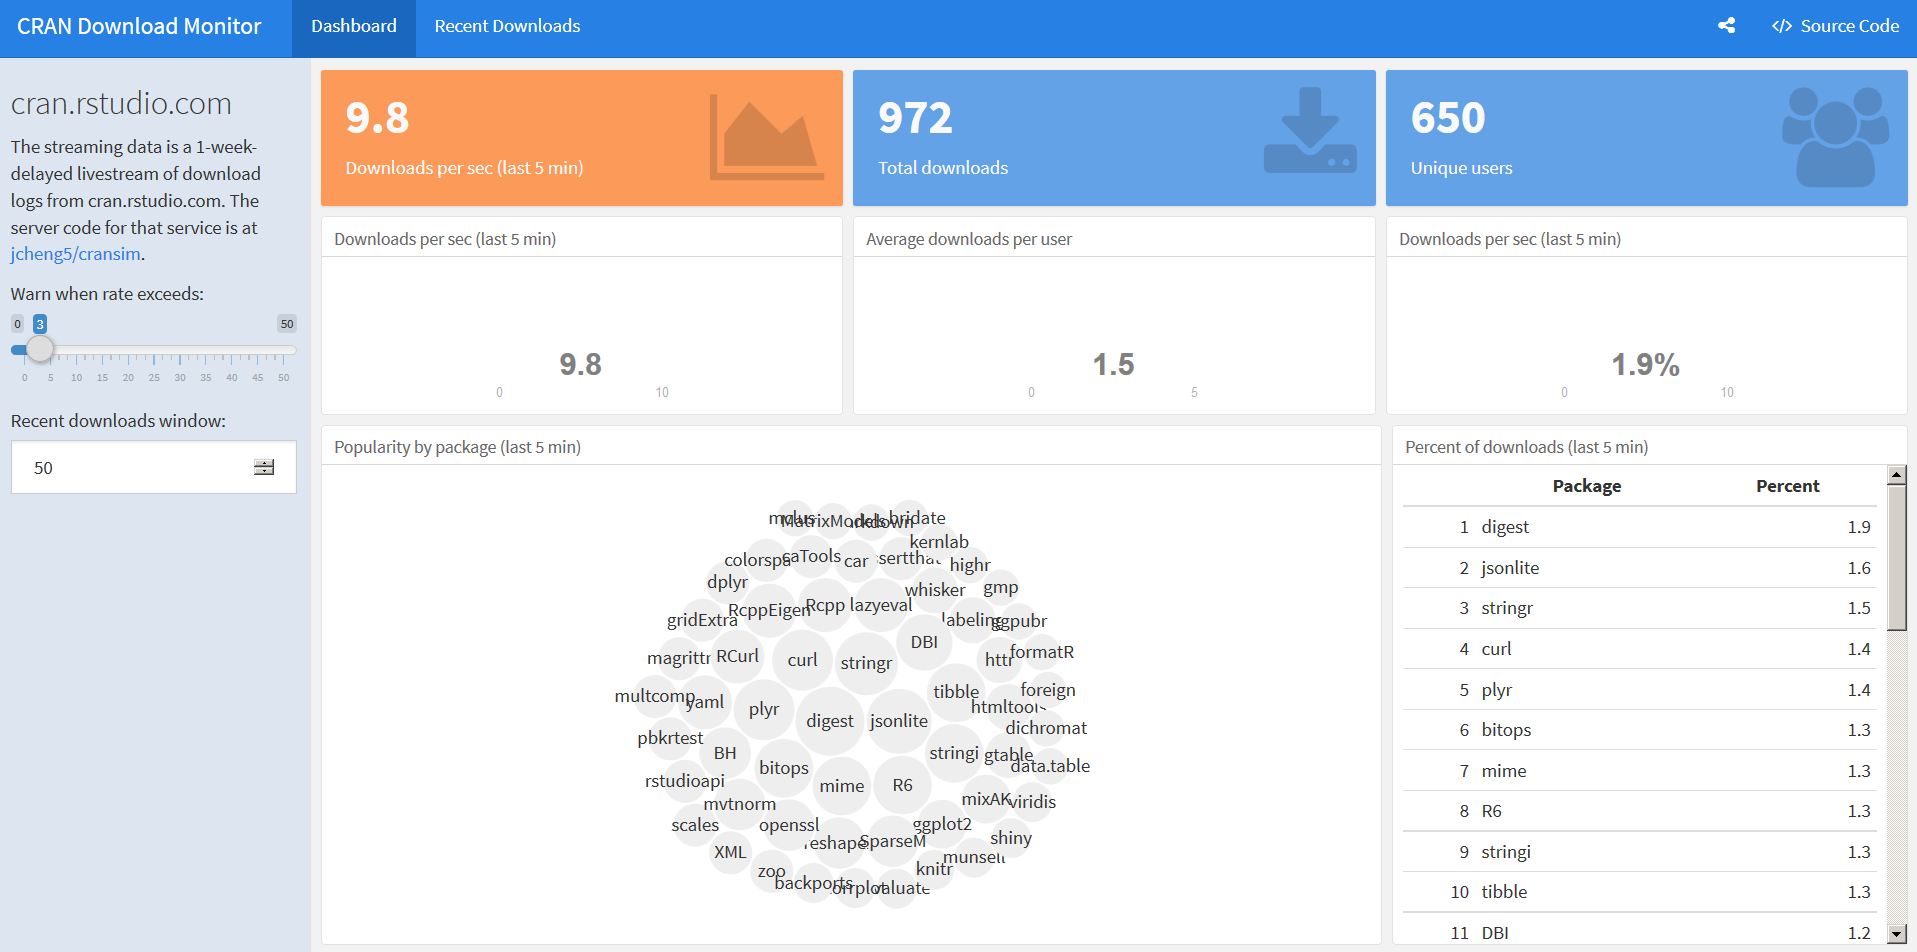
\includegraphics{D:/GitHub/IntroR/buildingblocks/figure/CRANdownloads.PNG}

\end{frame}

\begin{frame}{Download R:}
\protect\hypertarget{download-r}{}

\url{http://www.r-project.org/}

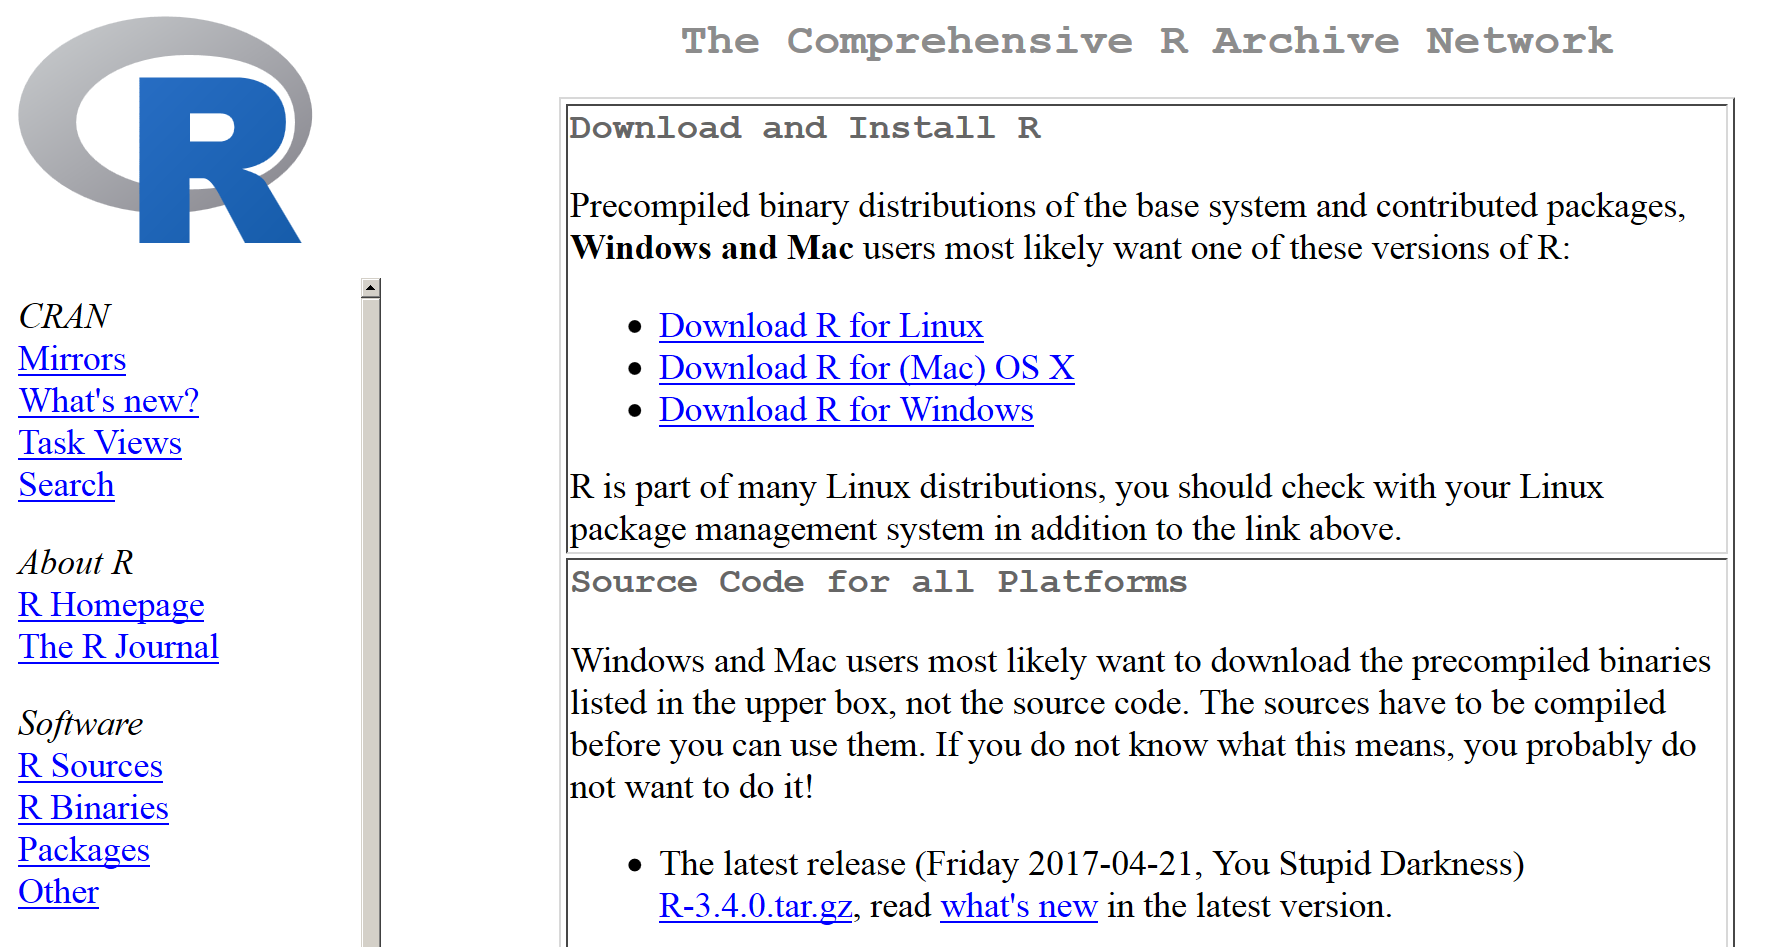
\includegraphics{D:/GitHub/IntroR/buildingblocks/figure/CRAN1picture.PNG}

\end{frame}

\begin{frame}{Open Source Programm R}
\protect\hypertarget{open-source-programm-r}{}

\begin{block}{Das ist das Basis-R:}

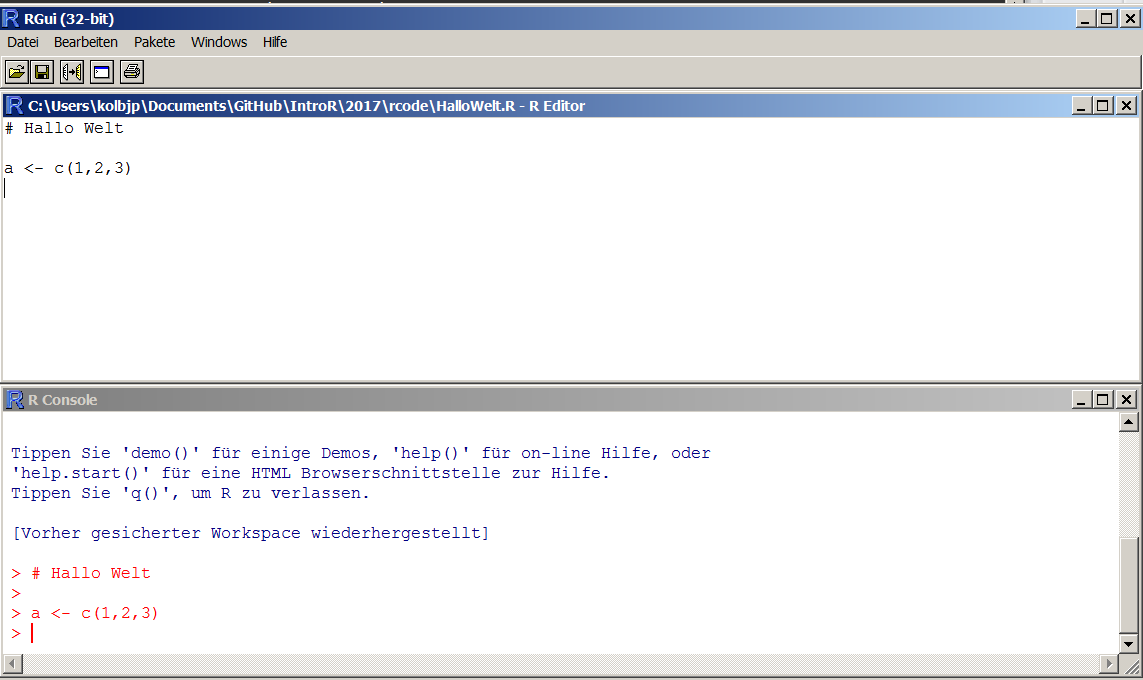
\includegraphics{D:/GitHub/IntroR/buildingblocks/figure/BasisR.PNG}

\end{block}

\end{frame}

\begin{frame}{Graphical user interface}
\protect\hypertarget{graphical-user-interface}{}

Viele Leute nutzen ein
\href{https://en.wikipedia.org/wiki/Graphical_user_interface}{\textbf{Graphical
User Interface}} (GUI) oder ein
\href{https://en.wikipedia.org/wiki/Integrated_development_environment}{\textbf{Integrated
Development Interface}} (IDE).

Aus den folgenden Gründen:

\begin{itemize}
\tightlist
\item
  Syntax-Hervorhebung
\item
  Auto-Vervollständigung
\item
  Bessere Übersicht über Graphiken, Pakete, Dateien, \ldots{}
\end{itemize}

\end{frame}

\begin{frame}{RStudio}
\protect\hypertarget{rstudio}{}

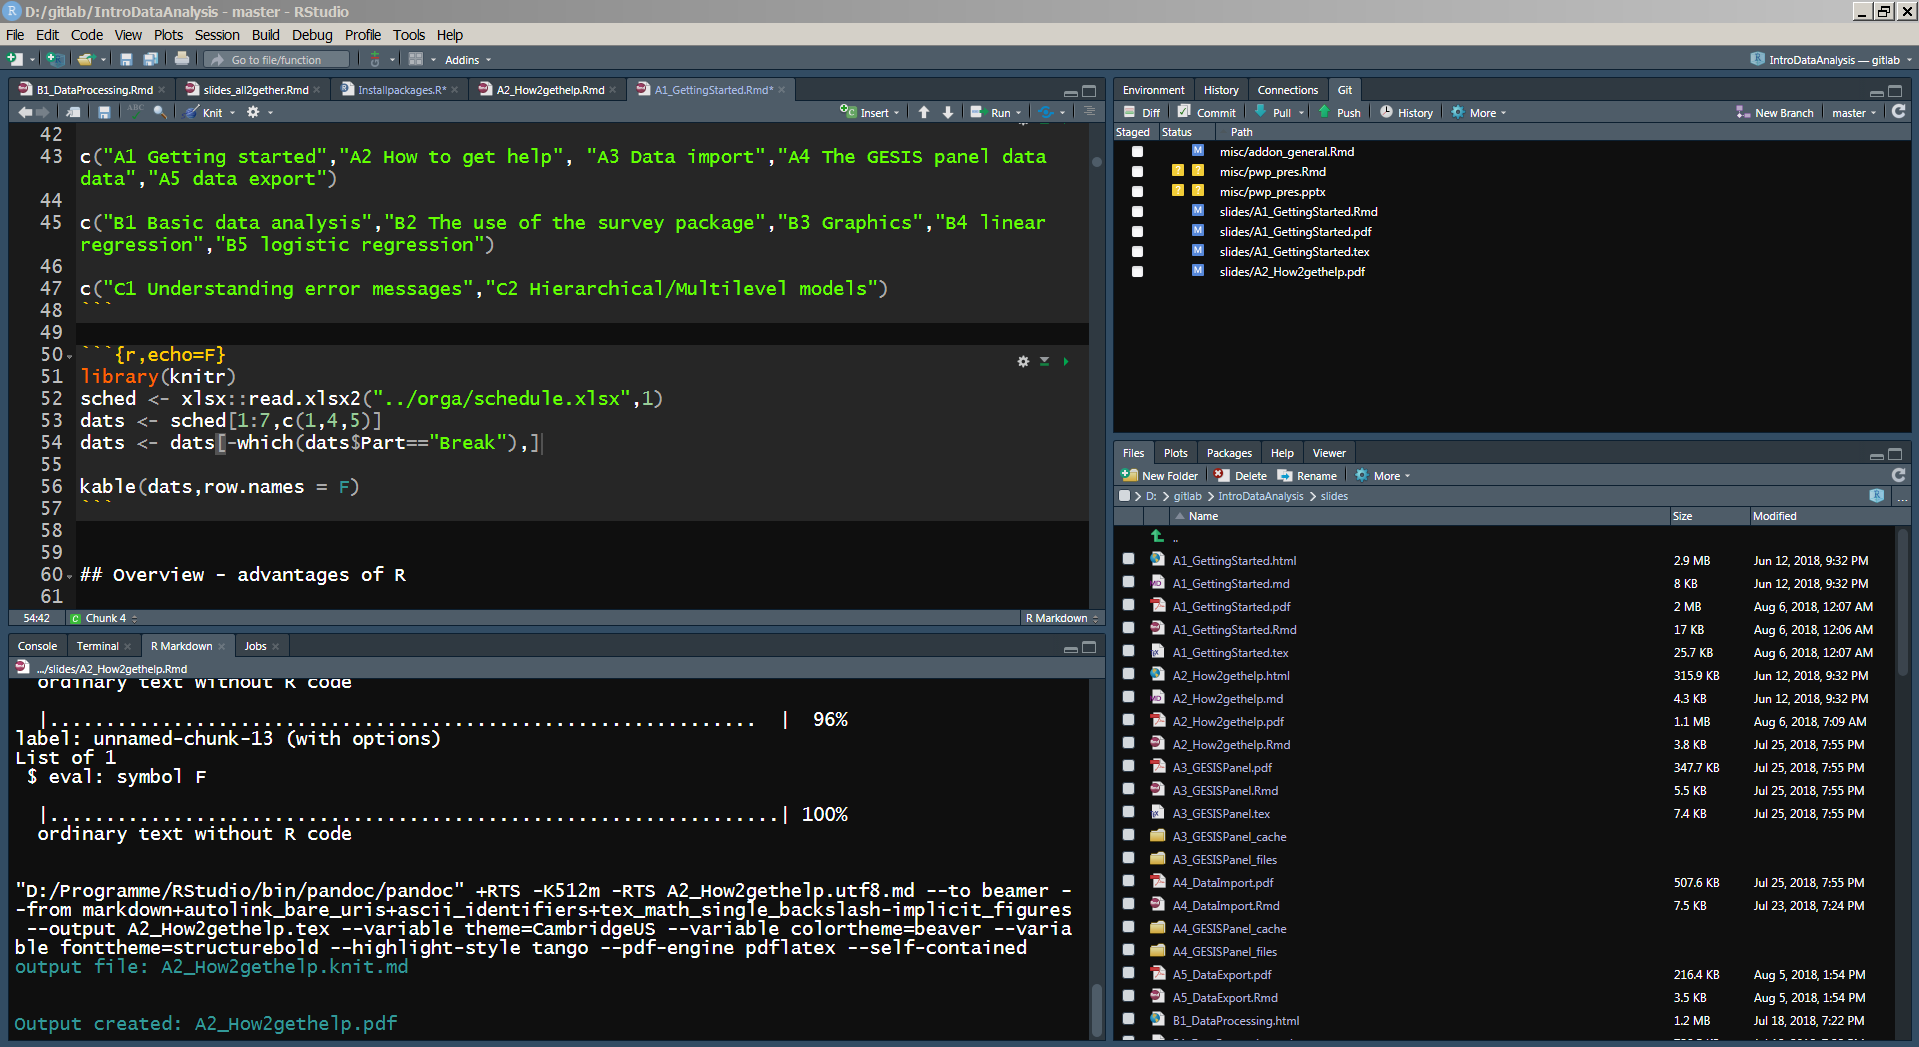
\includegraphics{D:/GitHub/IntroR/buildingblocks/figure/RstudioExample.PNG}

\end{frame}

\begin{frame}[fragile]{Übung - Vorbereitung}
\protect\hypertarget{ubung---vorbereitung}{}

\begin{itemize}
\item
  Schaue, ob R auf dem Computer installiert ist
\item
  Wenn nicht, lade \href{r-project.org}{\textbf{R}} herunter und
  installiere es.
\item
  Prüfe ob Rstudio installiert ist.
\item
  Wenn nicht - \href{http://www.rstudio.com/}{\textbf{installiere}}
  Rstudio.
\item
  Starte RStudio. Gehe in die Konsole (meistens Fenster unten links) und
  tippe
\item
  Erzeuge ein neues R Script (Ctrl + Shift + N)
\item
  Das Datum bekommt man mit der Funktion \texttt{date()} und die R
  Version mit \texttt{sessionInfo()}.
\end{itemize}

\end{frame}

\hypertarget{erste-schritte-mit-r}{%
\section{Erste Schritte mit R}\label{erste-schritte-mit-r}}

\begin{frame}[fragile]{R ist eine objektorientierte Sprache.}
\protect\hypertarget{r-ist-eine-objektorientierte-sprache.}{}

\begin{block}{Vektoren und Zuweisungen}

\begin{itemize}
\tightlist
\item
  \texttt{\textless{}-} ist der Zuweisungsoperator
\end{itemize}

\begin{Shaded}
\begin{Highlighting}[]
\NormalTok{b <-}\StringTok{ }\KeywordTok{c}\NormalTok{(}\DecValTok{1}\NormalTok{,}\DecValTok{2}\NormalTok{) }\CommentTok{# create an object with the numbers 1 and 2}
\end{Highlighting}
\end{Shaded}

\begin{itemize}
\tightlist
\item
  Auf dieses Objekt kann eine Funktion angewendet werden:
\end{itemize}

\begin{Shaded}
\begin{Highlighting}[]
\KeywordTok{mean}\NormalTok{(b) }\CommentTok{# computes the mean}
\end{Highlighting}
\end{Shaded}

\begin{verbatim}
## [1] 1.5
\end{verbatim}

Mit diesen Funktionen können wir etwas über die Eigenschaften des
Objekts erfahren:

\begin{Shaded}
\begin{Highlighting}[]
\KeywordTok{length}\NormalTok{(b) }\CommentTok{# b has the length 2}
\end{Highlighting}
\end{Shaded}

\begin{verbatim}
## [1] 2
\end{verbatim}

\end{block}

\begin{block}{Objektstruktur}

\begin{Shaded}
\begin{Highlighting}[]
\KeywordTok{str}\NormalTok{(b) }\CommentTok{# b is a numeric vector}
\end{Highlighting}
\end{Shaded}

\begin{verbatim}
##  num [1:2] 1 2
\end{verbatim}

\end{block}

\end{frame}

<<<<<<< HEAD
\begin{frame}[fragile]{Übung - Zuweisungen und Funktionen}
\protect\hypertarget{ubung---zuweisungen-und-funktionen}{}
=======
\begin{frame}[fragile]{Übung - Zuweisungen}
>>>>>>> 01469a2fc21a4ee08106a146f700460dce05e2c7

Erstelle einen Vektor \texttt{b} mit den Zahlen von 1 bis 5 und
berechne\ldots{}.

\begin{enumerate}
\item
  den Mittelwert
\item
  die Varianz
\item
  die Standardabweichung
\item
  die Quadratwurzel aus dem Mittelwert
\end{enumerate}

\end{frame}

\hypertarget{hilfe-bekommen}{%
\section{Hilfe bekommen}\label{hilfe-bekommen}}

\begin{frame}[fragile]{Wie bekomme ich Hilfe?}
\protect\hypertarget{wie-bekomme-ich-hilfe}{}

\begin{itemize}
\tightlist
\item
  \href{http://itfeature.com/tag/how-to-get-help-in-r}{\textbf{Um Hilfe
  im Allgemeinen zu bekommen:}}
\end{itemize}

\begin{Shaded}
\begin{Highlighting}[]
\KeywordTok{help.start}\NormalTok{()}
\end{Highlighting}
\end{Shaded}

\begin{itemize}
\tightlist
\item
  \href{https://www.r-project.org/help.html}{\textbf{Online-Dokumentation
  für die meisten Funktionen:}}
\end{itemize}

\begin{Shaded}
\begin{Highlighting}[]
\KeywordTok{help}\NormalTok{(name)}
\end{Highlighting}
\end{Shaded}

\begin{itemize}
\tightlist
\item
  Benutze \texttt{?}, um Hilfe zu bekommen
\end{itemize}

\begin{Shaded}
\begin{Highlighting}[]
\NormalTok{?mean}
\end{Highlighting}
\end{Shaded}

\begin{itemize}
\tightlist
\item
  \texttt{example(lm)} liefert ein Beispiel für die lineare Regression
\end{itemize}

\begin{Shaded}
\begin{Highlighting}[]
\KeywordTok{example}\NormalTok{(lm)}
\end{Highlighting}
\end{Shaded}

\end{frame}

\begin{frame}[fragile]{Vignetten}
\protect\hypertarget{vignetten}{}

\begin{itemize}
\tightlist
\item
  Eine Vignette ist ein Papier, das die wichtigsten Funktionen eines
  Pakets darstellt.
\item
  Sie enthalten viele reproduzierbare Beispiele.
\item
  Vignetten sind ein neues Werkzeug, deshalb hat nicht jedes Paket eine
  Vignette.
\end{itemize}

\begin{Shaded}
\begin{Highlighting}[]
\KeywordTok{browseVignettes}\NormalTok{()}
\end{Highlighting}
\end{Shaded}

\begin{itemize}
\tightlist
\item
  Um eine Vignette zu bekommen:
\end{itemize}

\begin{Shaded}
\begin{Highlighting}[]
\KeywordTok{vignette}\NormalTok{(}\StringTok{"osmdata"}\NormalTok{)}
\end{Highlighting}
\end{Shaded}

\end{frame}

\begin{frame}{Ein Beispiel für eine Vignette - Das Paket
\texttt{osmdata}}
\protect\hypertarget{ein-beispiel-fur-eine-vignette---das-paket-osmdata}{}

\includegraphics{D:/GitHub/IntroR/buildingblocks/figure/ex_osmdata_vignette.PNG}

\end{frame}

\begin{frame}[fragile]{\href{http://r-pkgs.had.co.nz/demo.html}{\textbf{Demos}}}
\protect\hypertarget{demos}{}

\begin{itemize}
\tightlist
\item
  für manche Pakete gibt es Demos:
\end{itemize}

\begin{Shaded}
\begin{Highlighting}[]
\KeywordTok{demo}\NormalTok{() }\CommentTok{# zeigt alle verfügbaren Demos}
\KeywordTok{demo}\NormalTok{(}\DataTypeTok{package =} \StringTok{"httr"}\NormalTok{) }\CommentTok{# Zeigt alle Demos in einem Paket}

\CommentTok{# Ein spezifisches Demo laufen lassen:}
\KeywordTok{demo}\NormalTok{(}\StringTok{"oauth1-twitter"}\NormalTok{, }\DataTypeTok{package =} \StringTok{"httr"}\NormalTok{) }
\end{Highlighting}
\end{Shaded}

\begin{itemize}
\tightlist
\item
  Wenn ein Demo gestartet wird, ist der zugehörige Code in der Konsole
  sichtbar
\end{itemize}

\begin{Shaded}
\begin{Highlighting}[]
\KeywordTok{demo}\NormalTok{(nlm)}
\end{Highlighting}
\end{Shaded}

\includegraphics{D:/GitHub/IntroR/buildingblocks/figure/demonlm.PNG}

\end{frame}

\begin{frame}[fragile]{Die Funktion \texttt{apropos}}
\protect\hypertarget{die-funktion-apropos}{}

\begin{itemize}
\tightlist
\item
  durchsucht alles über den angegebenen String:
\end{itemize}

\begin{Shaded}
\begin{Highlighting}[]
\KeywordTok{apropos}\NormalTok{(}\StringTok{"lm"}\NormalTok{)}
\end{Highlighting}
\end{Shaded}

\begin{verbatim}
##  [1] ".colMeans"       ".lm.fit"         "colMeans"       
##  [4] "confint.lm"      "contr.helmert"   "dummy.coef.lm"  
##  [7] "getAllMethods"   "glm"             "glm.control"    
## [10] "glm.fit"         "KalmanForecast"  "KalmanLike"     
## [13] "KalmanRun"       "KalmanSmooth"    "kappa.lm"       
## [16] "lm"              "lm.fit"          "lm.influence"   
## [19] "lm.wfit"         "model.matrix.lm" "nlm"            
## [22] "nlminb"          "predict.glm"     "predict.lm"     
## [25] "residuals.glm"   "residuals.lm"    "summary.glm"    
## [28] "summary.lm"
\end{verbatim}

\begin{itemize}
\tightlist
\item
  Funktion kann auch mit
  \href{https://de.wikipedia.org/wiki/Regul\%C3\%A4rer_Ausdruck}{\textbf{regulären
  Ausdrücken}} verwendet werden\ldots{}
\end{itemize}

\begin{Shaded}
\begin{Highlighting}[]
\NormalTok{?}\StringTok{"regular expression"}
\end{Highlighting}
\end{Shaded}

\begin{Shaded}
\begin{Highlighting}[]
\KeywordTok{help.search}\NormalTok{(}\StringTok{"^glm"}\NormalTok{)}
\end{Highlighting}
\end{Shaded}

\begin{itemize}
\tightlist
\item
  \texttt{??} ist ein Synonym für \texttt{help.search}
\end{itemize}

\end{frame}

\begin{frame}[fragile]{\href{http://search.r-project.org/cgi-bin/namazu.cgi?query=glm\&max=20\&result=normal\&sort=score\&idxname=functions\&idxname=vignettes\&idxname=views}{\textbf{Suchmaschine
für die R-Seite}}}
\protect\hypertarget{suchmaschine-fur-die-r-seite}{}

\begin{Shaded}
\begin{Highlighting}[]
\KeywordTok{RSiteSearch}\NormalTok{(}\StringTok{"glm"}\NormalTok{)}
\end{Highlighting}
\end{Shaded}

\includegraphics{D:/GitHub/IntroR/buildingblocks/figure/rsitesearch.PNG}

\end{frame}

\begin{frame}[fragile]{Nutzung von Suchmaschinen}
\protect\hypertarget{nutzung-von-suchmaschinen}{}

\begin{itemize}
\tightlist
\item
  Ich nutze \href{}{\textbf{duckduckgo.de:}}
\end{itemize}

\begin{verbatim}
R-project + "was ich schon immer wissen wollte" 
\end{verbatim}

\begin{itemize}
\tightlist
\item
  das funktioniert natürlich für alle Suchmaschinen!
\end{itemize}

\includegraphics{D:/GitHub/IntroR/buildingblocks/figure/duckduckgo.PNG}

\end{frame}

\begin{frame}{\href{http://stackoverflow.com/}{\textbf{Stackoverflow}}}
\protect\hypertarget{stackoverflow}{}

\begin{itemize}
\tightlist
\item
  Für alle Fragen zum programmieren
\item
  Ist nicht auf R fokussiert - aber es gibt
  \href{https://stackoverflow.com/tags/r/info}{\textbf{viele
  Diskussionen zu R-Fragen}}
\item
  Sehr detailierte Diskussionen
\end{itemize}

\includegraphics{D:/GitHub/IntroR/buildingblocks/figure/StackoverflowEx.PNG}

\end{frame}

\begin{frame}{Ein Schummelzettel für Basis R}
\protect\hypertarget{ein-schummelzettel-fur-basis-r}{}

\url{https://www.rstudio.com/resources/cheatsheets/}

\includegraphics{D:/GitHub/IntroR/buildingblocks/figure/basercheatsheet.PNG}

\end{frame}

\begin{frame}{Mehr Schummelzettel}
\protect\hypertarget{mehr-schummelzettel}{}

\includegraphics{D:/GitHub/IntroR/buildingblocks/figure/cheatsheets.PNG}

\end{frame}

\begin{frame}{\href{http://www.statmethods.net/interface/help.html}{\textbf{Quick
R}}}
\protect\hypertarget{quick-r}{}

\begin{itemize}
\tightlist
\item
  Immer mit vielen Beispielen und Hilfen bezüglich eines Themas
\item
  Beispiel:
  \href{http://www.statmethods.net/interface/help.html}{\textbf{Quick R
  - Getting Help}}
\end{itemize}

\includegraphics{D:/GitHub/IntroR/buildingblocks/figure/quickR.PNG}

\end{frame}

\begin{frame}{Weitere Links}
\protect\hypertarget{weitere-links}{}

\begin{itemize}
\tightlist
\item
  \href{https://www.r-project.org/help.html}{\textbf{Überblick - wie
  bekommt man Hilfe in R}}
\end{itemize}

\includegraphics{D:/GitHub/IntroR/buildingblocks/figure/gettingHelp.PNG}

\begin{itemize}
\item
  \href{http://rprogramming.net/}{\textbf{Eine Liste mit HowTo`s}}
\item
  \href{https://www.personality-project.org/r/r.commands.html}{\textbf{Eine
  Liste mit den wichtigsten R-Befehlen}}
\end{itemize}

\end{frame}

\hypertarget{r-ist-modular}{%
\section{R ist modular}\label{r-ist-modular}}

\begin{frame}{\href{https://stats.idre.ucla.edu/r/seminars/intro/}{\textbf{Wo
man Routinen findet}}}
\protect\hypertarget{wo-man-routinen-findet}{}

\begin{itemize}
\tightlist
\item
  Viele Funktionen sind in Basis-R enthalten.
\item
  Viele spezifische Funktionen sind in zusätzliche Bibliotheken
  integriert.
\item
  R kann modular durch sogenannte Pakete oder Bibliotheken erweitert
  werden.
\item
<<<<<<< HEAD
  Die wichtigsten Pakete, die auf CRAN gehostet werden (13640 at Do 10
=======
  Die wichtigsten Pakete, die auf CRAN gehostet werden (13641 at Do 10
>>>>>>> 01469a2fc21a4ee08106a146f700460dce05e2c7
  Jan 2019)
\item
  Weitere Pakete findet man z.B. unter
  \href{www.bioconductor.org}{\textbf{bioconductor}}
\end{itemize}

\end{frame}

\begin{frame}{\href{https://www.youtube.com/watch?v=kKI9--Opmso}{Übersicht
R-Pakete}}
\protect\hypertarget{ubersicht-r-pakete}{}

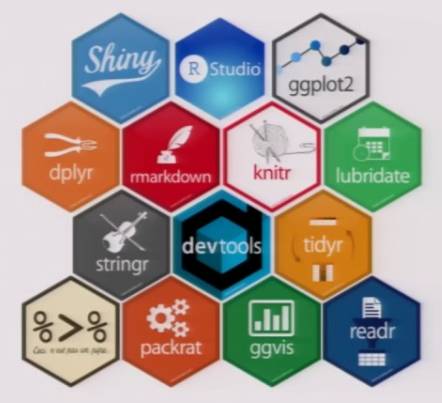
\includegraphics{figure/packages_overview.PNG}

\end{frame}

\begin{frame}[fragile]{Installation von Paketen}
\protect\hypertarget{installation-von-paketen}{}

\begin{itemize}
\tightlist
\item
  Die Anführungszeichen um den Paketnamen herum sind für den Befehl
  \texttt{install.packages} notwendig.
\item
  Sie sind optional für den Befehl \texttt{library}.
\item
  Man kann auch \texttt{require} anstelle von \texttt{library}
  verwenden.
\end{itemize}

\begin{Shaded}
\begin{Highlighting}[]
\KeywordTok{install.packages}\NormalTok{(}\StringTok{"raster"}\NormalTok{)}

\KeywordTok{library}\NormalTok{(raster)}
\end{Highlighting}
\end{Shaded}

\end{frame}

\begin{frame}{Installation von Paketen mit RStudio}
\protect\hypertarget{installation-von-paketen-mit-rstudio}{}

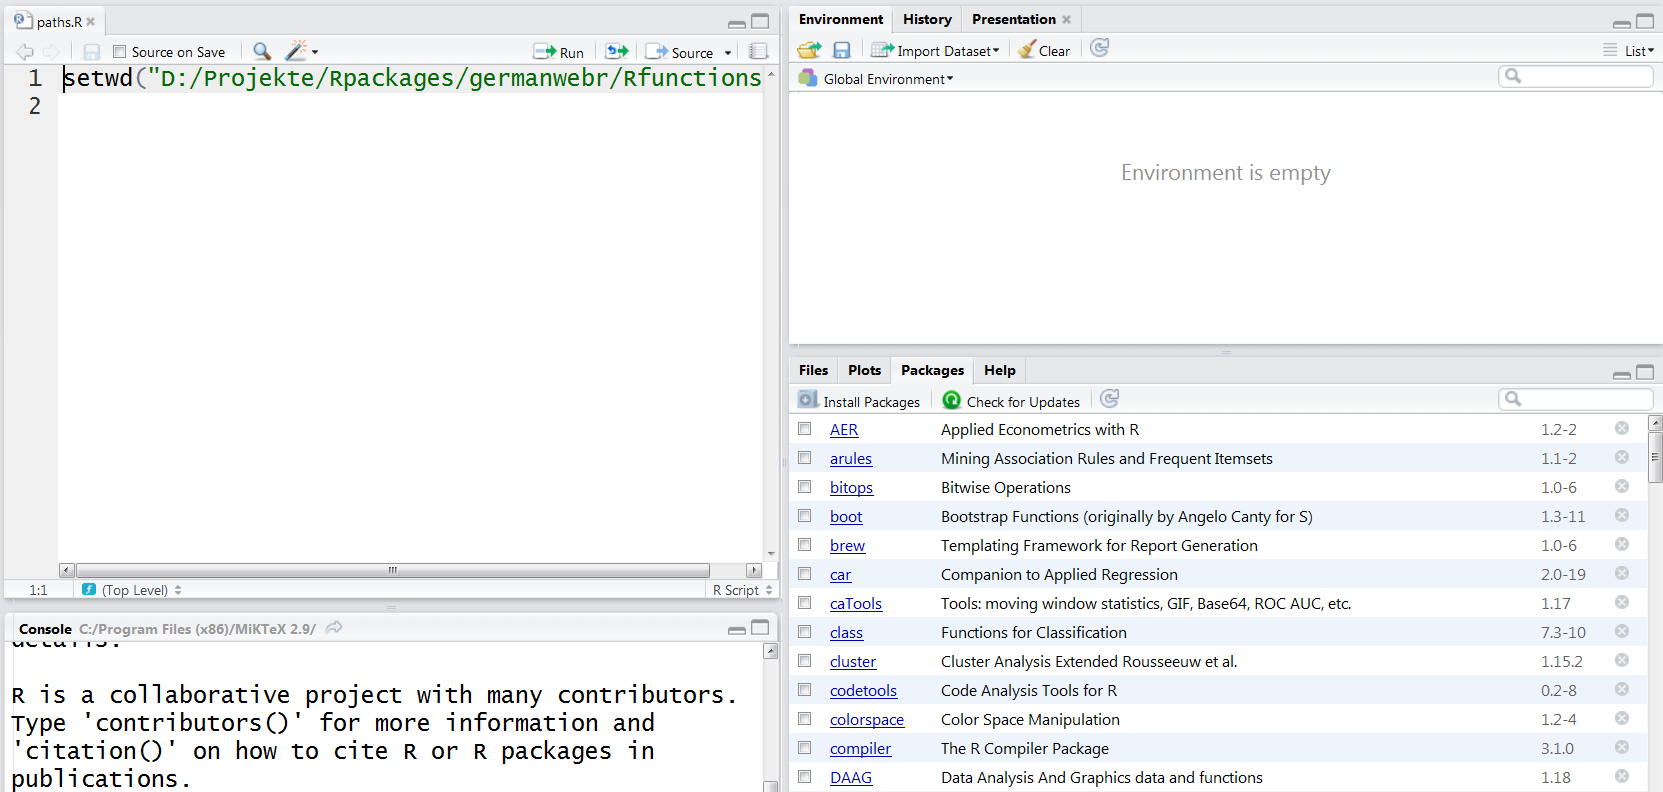
\includegraphics{figure/PaketeRstudio.PNG}

\end{frame}

\begin{frame}{Bestehende Pakete und Installation}
\protect\hypertarget{bestehende-pakete-und-installation}{}

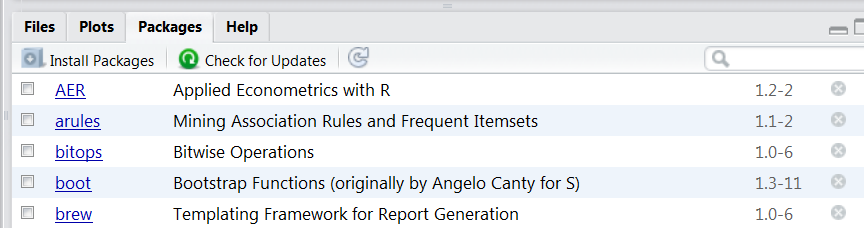
\includegraphics{figure/packages3.PNG}

\end{frame}

\begin{frame}[fragile]{Übersicht Pakete:}
\protect\hypertarget{ubersicht-pakete}{}

\begin{itemize}
\tightlist
\item
  Luhmann -
  \href{http://www.beltz.de/fileadmin/beltz/downloads/OnlinematerialienPVU/28090_Luhmann/Verwendete\%20Pakete.pdf}{\textbf{Übersicht
  mit vielen nützlichen Paketen}}
\item
  Mit dem Paket \texttt{leaflet} kann man interaktive Karten erstellen.
\item
  Das Paket \texttt{tmap} zur Erstellung von thematischen Karten.
\item
  \href{http://www.r-bloggers.com/tag/maptools/}{\textbf{Paket
  \texttt{maptools} um Karten zu erzeugen}}
\item
  Das Paket \texttt{sf} - bietet Zugang zu
  \href{https://de.wikipedia.org/wiki/Simple_Feature_Access}{\textbf{simple
  features}}.
\end{itemize}


\includegraphics{figure/logo_sf.PNG}

\end{frame}

\begin{frame}[fragile]{Pakete aus verschiedenen Quellen installieren}
\protect\hypertarget{pakete-aus-verschiedenen-quellen-installieren}{}

\begin{block}{Pakete vom CRAN Server installieren}

\begin{Shaded}
\begin{Highlighting}[]
\KeywordTok{install.packages}\NormalTok{(}\StringTok{"lme4"}\NormalTok{)}
\end{Highlighting}
\end{Shaded}

\end{block}

\begin{block}{Pakete vom Bioconductor Server installieren}

\begin{Shaded}
\begin{Highlighting}[]
\KeywordTok{source}\NormalTok{(}\StringTok{"https://bioconductor.org/biocLite.R"}\NormalTok{)}
\KeywordTok{biocLite}\NormalTok{(}\KeywordTok{c}\NormalTok{(}\StringTok{"GenomicFeatures"}\NormalTok{, }\StringTok{"AnnotationDbi"}\NormalTok{))}
\end{Highlighting}
\end{Shaded}

\end{block}

\begin{block}{Pakete von Github installieren}

\begin{Shaded}
\begin{Highlighting}[]
\KeywordTok{install.packages}\NormalTok{(}\StringTok{"devtools"}\NormalTok{)}
\KeywordTok{library}\NormalTok{(devtools)}

\KeywordTok{install_github}\NormalTok{(}\StringTok{"hadley/maptools"}\NormalTok{)}
\end{Highlighting}
\end{Shaded}

\end{block}

\end{frame}

\begin{frame}{Wie bekomme ich einen Überblick?}
\protect\hypertarget{wie-bekomme-ich-einen-uberblick}{}

\begin{itemize}
\item
  Entdecke Pakete, die kürzlich auf den
  \href{https://mran.microsoft.com/packages/}{\textbf{CRAN}} Server
  hochgeladen wurden
\item
  Nutze eine Shiny Web-App, in der
  \href{https://gallery.shinyapps.io/cran-gauge/}{\textbf{Pakete
  angezeigt werden, die kürzlich von CRAN}} heruntergeladen wurden.
\item
  Werfe einen Blick auf eine
  \href{https://support.rstudio.com/hc/en-us/articles/201057987-Quick-list-of-useful-R-packages}{\textbf{Quick-Liste
  nützlicher Pakete}}
\item
  \ldots{}., oder auf eine Liste mit den
  \href{http://www.computerworld.com/article/2921176/business-intelligence/great-r-packages-for-data-import-wrangling-visualization.html}{\textbf{besten
  Paketen für die Datenverarbeitung und -analyse}},\ldots{}..
\item
  \ldots{}., oder sieh Dir
  \href{https://www.r-bloggers.com/the-50-most-used-r-packages/}{\textbf{die
  50 meistgenutzten Pakete}} an.
\end{itemize}

\end{frame}

\begin{frame}[fragile]{CRAN Task Views}
\protect\hypertarget{cran-task-views}{}

\begin{itemize}
\tightlist
\item
  Bezüglich mancher Themen gibt es einen Überblick über alle wichtigen
  Pakete - (\href{https://cran.r-project.org/web/views/}{\textbf{CRAN
  Task Views}})
\item
  Momentan gibt es 35 Task Views.
\item
  Alle Pakete einer Task-View können mit folgendem Befehl installiert
  werden:
  \href{https://mran.microsoft.com/rpackages/}{\textbf{command:}}
\end{itemize}

\begin{Shaded}
\begin{Highlighting}[]
\KeywordTok{install.packages}\NormalTok{(}\StringTok{"ctv"}\NormalTok{)}
\KeywordTok{library}\NormalTok{(}\StringTok{"ctv"}\NormalTok{)}
\KeywordTok{install.views}\NormalTok{(}\StringTok{"Spatial"}\NormalTok{)}
\end{Highlighting}
\end{Shaded}

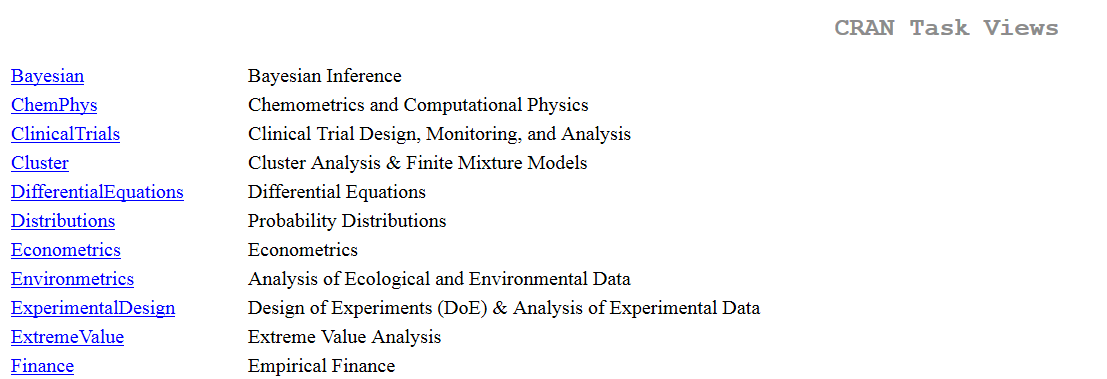
\includegraphics{figure/CRANtaskViews.PNG}

\end{frame}

\begin{frame}{Übung - zusätzliche Pakete}
\protect\hypertarget{ubung---zusatzliche-pakete}{}

Geh bspw. auf \url{https://cran.r-project.org/} und suche nach
Paketen\ldots{}

\begin{itemize}
\tightlist
\item
  die sich für interaktive Karten eignen.
\item
  mit denen man thematische Karten erstellen kann
\item
  mit denen man die räumliche Distanz berechnen kann
\item
  mit denen man eine Satellitenkarte bekommen kann
\end{itemize}

\end{frame}

<<<<<<< HEAD
\hypertarget{erste-karten}{%
\section{Erste Karten}\label{erste-karten}}

\begin{frame}[fragile]{Das Paket maptools}
\protect\hypertarget{das-paket-maptools}{}
=======
\section{Warum die räumliche
Perspektive}\label{warum-die-raumliche-perspektive}

\begin{frame}{Warum die Darstellung in Karten}

\begin{itemize}
\item
  Darstellung in Karten ermöglicht besseres Verständnis von
  sozialwissenschaftlicher Phänomene - Attraktiver Output
\item
  Durch die INSPIRE Richtlinie und \emph{Collaborative Mapping} wächst
  der verfügbare Bestand an Geodaten.
\item
  Daten sind oft frei verfügbar im Internet (z.B. Nutzung von APIs)
\item
  Allerdings sind die Daten oft wenig strukturiert, heterogen oder nicht
  zur räumlichen Visualisierung vorgesehen
\item
  beinhalten aber implizit geographische Informationen (Web 2.0)
\item
  Oftmals sind wenig oder keine Metadaten vorhanden
\end{itemize}

\end{frame}

\begin{frame}{\href{https://www.ratswd.de/dl/downloads/RatSWD_Geodatenbericht.pdf}{Das
Thema Geodatenlandschaft}}


\includegraphics{D:/Daten/GitHub/IntroR/buildingblocks/figure/BildRatSWDBericht.png}

\end{frame}

\begin{frame}{Was heißt das für diesen Kurs}

\begin{block}{Vorgestellt werden:}
>>>>>>> 01469a2fc21a4ee08106a146f700460dce05e2c7

\begin{itemize}
\tightlist
\item
  Möglichkeiten für den Download, den Import, die Verarbeitung und die
  Visualisierung von Geodaten
\end{itemize}

\begin{itemize}
\tightlist
\item
  Quellen für Geodaten
\item
  Eine Programmierschnittstelle (APIs) um die Daten zu bekommen
\item
  R-Pakete um diese Daten zu verarbeiten und zu visualisieren
\end{itemize}

\end{block}

\end{frame}

\section{OpenStreetMap}\label{openstreetmap}

\begin{frame}{Inhalt dieses Abschnitts}

\begin{itemize}
\tightlist
\item
  Vorstellung des Openstreetmap (OSM) Projekts
\item
  Welche OSM-Daten sind erhältlich und wie kann man diese bekommen?
\item
  Präsentation des Key-Value Schemas, dass bei OSM Daten verwendet wird.
\end{itemize}

\end{frame}

\begin{frame}{\href{http://www.openstreetmap.de/}{OpenStreetMap}
Projekt}

\begin{block}{\url{http://www.openstreetmap.de/}}

\begin{quote}
OpenStreetMap.org ist ein im Jahre 2004 gegründetes internationales
Projekt mit dem Ziel, eine freie Weltkarte zu erschaffen. Dafür sammeln
wir weltweit Daten über Straßen, Eisenbahnen, Flüsse, Wälder, Häuser und
vieles mehr.
\end{quote}

\end{block}

\end{frame}

\begin{frame}{OpenStreetMap}

\begin{block}{\href{https://en.wikipedia.org/wiki/OpenStreetMap}{\textbf{Wikipedia
- OpenStreetMap}}}

\begin{quote}
OpenStreetMap (OSM) ist ein kollaboratives Projekt um eine editierbare
Weltkarte zu erzeugen.
\end{quote}

\includegraphics{D:/Daten/GitHub/IntroR/buildingblocks/figure/overview_osm.PNG}

\end{block}

\end{frame}

\begin{frame}[fragile]{\href{https://wiki.openstreetmap.org/wiki/Tags}{Openstreetmap
Tags}}

\includegraphics{D:/Daten/GitHub/IntroR/buildingblocks/figure/kv_scheme.PNG}

\begin{itemize}
\tightlist
\item
  Mit dem \texttt{key} wird eine Kategorie bezeichnet.
\item
  Der \texttt{value} wird zur Beschreibung der jeweiligen Form
  verwendet.
\item
  So gibt es bspw. zahlreiche OSM-Objekte mit dem \texttt{key} highway.
  Dabei kann es sich bspw. um einen Fußweg (value=pathway) oder um eine
  Autobahn (value=motorway) handeln.
\end{itemize}

\end{frame}

\begin{frame}{\href{http://wiki.openstreetmap.org/wiki/DE:Map_Features}{OSM
Map Features}}

\includegraphics{D:/Daten/GitHub/IntroR/buildingblocks/figure/osm_mapfeatures.png}

\end{frame}

\begin{frame}{Objekttypen in OSM}

\begin{block}{Es gibt prinipiell drei verschiedene Objekttypen:}

\begin{itemize}
\tightlist
\item
  Es gibt einfache nodes, also Punkte. Das kann bspw. eine Haltestelle
  des öffentlichen Nahverkehrs sein.
\item
  Der zweite Objekttyp sind Wege. Dadurch wird beispielsweise der
  Verlauf von Straßen oder Flüssen beschrieben.
\item
  Der dritte Objekttyp sind Relationen. Dabei handelt es sich um eine
  Gruppierung von Objekten, die in einem logischen Zusammenhang stehen.
\end{itemize}

Hippolyte Pruvost and Peter Mooney: Exploring Data Model Relations in
OpenStreetMap

\end{block}

\end{frame}

\begin{frame}{OpenStreetMap objects}

\begin{block}{\href{https://www.slideshare.net/mvexel/openstreetmap-9819440}{\textbf{Martijn
van Exel}} - nodes and ways}

\includegraphics{D:/Daten/GitHub/IntroR/buildingblocks/figure/Nodes_ways.PNG})

\end{block}

\end{frame}

\begin{frame}{OpenStreetMap objects}

\begin{block}{Relations}

\includegraphics{D:/Daten/GitHub/IntroR/buildingblocks/figure/relations.PNG})

\end{block}

\end{frame}

\begin{frame}{Möglichkeiten die OSM-Daten zu bekommen}

\begin{itemize}
\tightlist
\item
  Es gibt verschiedene Möglichkeiten die OSM-Daten zu bekommen.
\item
  Metro Extracts bietet rechteckige Ausschnitte für eine Stadt oder
  Region von Interesse auf der ganzen Welt.
\item
  Grundsätzlich werden die Rohdaten im \emph{Protocolbuffer Binary
  Format} (PBF) oder im \emph{Extensible Markup Language} (XML) Format
  angeboten.
\item
  Die
  \href{https://de.wikipedia.org/wiki/Keyhole_Markup_Language}{\textbf{Keyhole
  Markup Language}} (KML) ist eine Auszeichnungssprache zur Beschreibung
  von Geodaten. Diese wurde bei Google Earth angewendet. KML befolgt die
  XML-Syntax.
\end{itemize}

\end{frame}

\begin{frame}{Download von OpenStreetMap Daten -
\href{https://mapzen.com/}{Metro extracts}}

\begin{itemize}
\tightlist
\item
  Ausschnitte von OpenStreetMap für einzelne Städte
  (\href{https://mapzen.com/data/metro-extracts/}{\textbf{metro
  extracts}})
\end{itemize}

\includegraphics{D:/Daten/GitHub/IntroR/buildingblocks/figure/metroextracts.png})

\end{frame}

\begin{frame}{Download von OpenStreetMap Daten - Geofabrik}

\begin{block}{Geofabrik}

\begin{itemize}
\tightlist
\item
  Eine Alternative zum Downlaod von großen OSM-Ausschnitten ist die
  \href{http://download.geofabrik.de/}{\textbf{Geofabrik}}-Seite.\\
\item
  Hier lassen sich ebenfalls aktuelle Ausschnitte aber auch Shapefiles
  herunterladen.
\end{itemize}

\includegraphics{D:/Daten/GitHub/IntroR/buildingblocks/figure/Geofabrik.PNG})

\end{block}

\end{frame}

\begin{frame}{OSM Planet file}

\begin{block}{Datenbanklösungen}

\begin{itemize}
\tightlist
\item
  Bei den eben vorgestellten Möglichkeiten geht es vor allem um das
  Herunterladen kleiner Ausschnitte.
\item
  Wenn größere Datenmengen benötigt werden, sollte man eine
  Datenbanklösung nutzen.
\item
  \href{http://www.postgresql.org/}{\textbf{PostgreSQL}} hat den
  Vorteil, dass es Open-Source ist.
\end{itemize}

\end{block}

\end{frame}

\begin{frame}{\href{http://www.postgresql.org/download/windows/}{Download
PostgreSQL}}

\begin{itemize}
\tightlist
\item
  \href{https://datashenanigan.wordpress.com/2015/05/18/getting-started-with-postgresql-in-r/}{\textbf{Hier}}
  ist eine Einführung in PostgreSQL zu finden
\end{itemize}

\includegraphics{D:/Daten/GitHub/IntroR/buildingblocks/figure/aquadatastudio_postgresql_visual_table_editing.png})

\end{frame}

<<<<<<< HEAD
\begin{frame}[fragile]{Hello world}
\protect\hypertarget{hello-world}{}
=======
\begin{frame}{pgAdmin}

\begin{itemize}
\tightlist
\item
  Sehr empfehlenswert: Arbeiten mit
  \href{https://www.pgadmin.org/}{\textbf{pgAdmin}}
\item
  Beispiel: um Verknüpfung zu einer Datenbank herzustellen - Doppelklick
  auf den Server in pgAdmin
\end{itemize}

\end{frame}

\begin{frame}[fragile]{PostGIS für PostgreSQL}

\begin{itemize}
\tightlist
\item
  \href{http://postgis.net/install/}{\textbf{Installieren}} der PostGIS
  Erweiterung:
\end{itemize}

\begin{verbatim}
CREATE EXTENSION postgis;
\end{verbatim}

\includegraphics{D:/Daten/GitHub/IntroR/buildingblocks/figure/PostGIS_logo.png})

\end{frame}

\begin{frame}[fragile]{Programm zum Import der OSM Daten in PostgreSQL-
osm2pgsql}

\begin{itemize}
\tightlist
\item
  Läuft unter Linux deutlich besser
\item
  so könnte bspw. ein Import in PostgreSQL aussehen:
\end{itemize}

\begin{verbatim}
osm2pgsql -c -d osmBerlin --slim -C  -k  berlin-latest.osm.pbf
\end{verbatim}

\end{frame}

\begin{frame}[fragile]{Verbindung zwischen R und Postrgesql}

\begin{block}{\href{https://github.com/tomoakin/RPostgreSQL}{\textbf{Github
Verzeichnis}} zum Paket}
>>>>>>> 01469a2fc21a4ee08106a146f700460dce05e2c7

\begin{Shaded}
\begin{Highlighting}[]
\KeywordTok{install.packages}\NormalTok{(}\StringTok{"RPostgreSQL"}\NormalTok{)}
\end{Highlighting}
\end{Shaded}

<<<<<<< HEAD
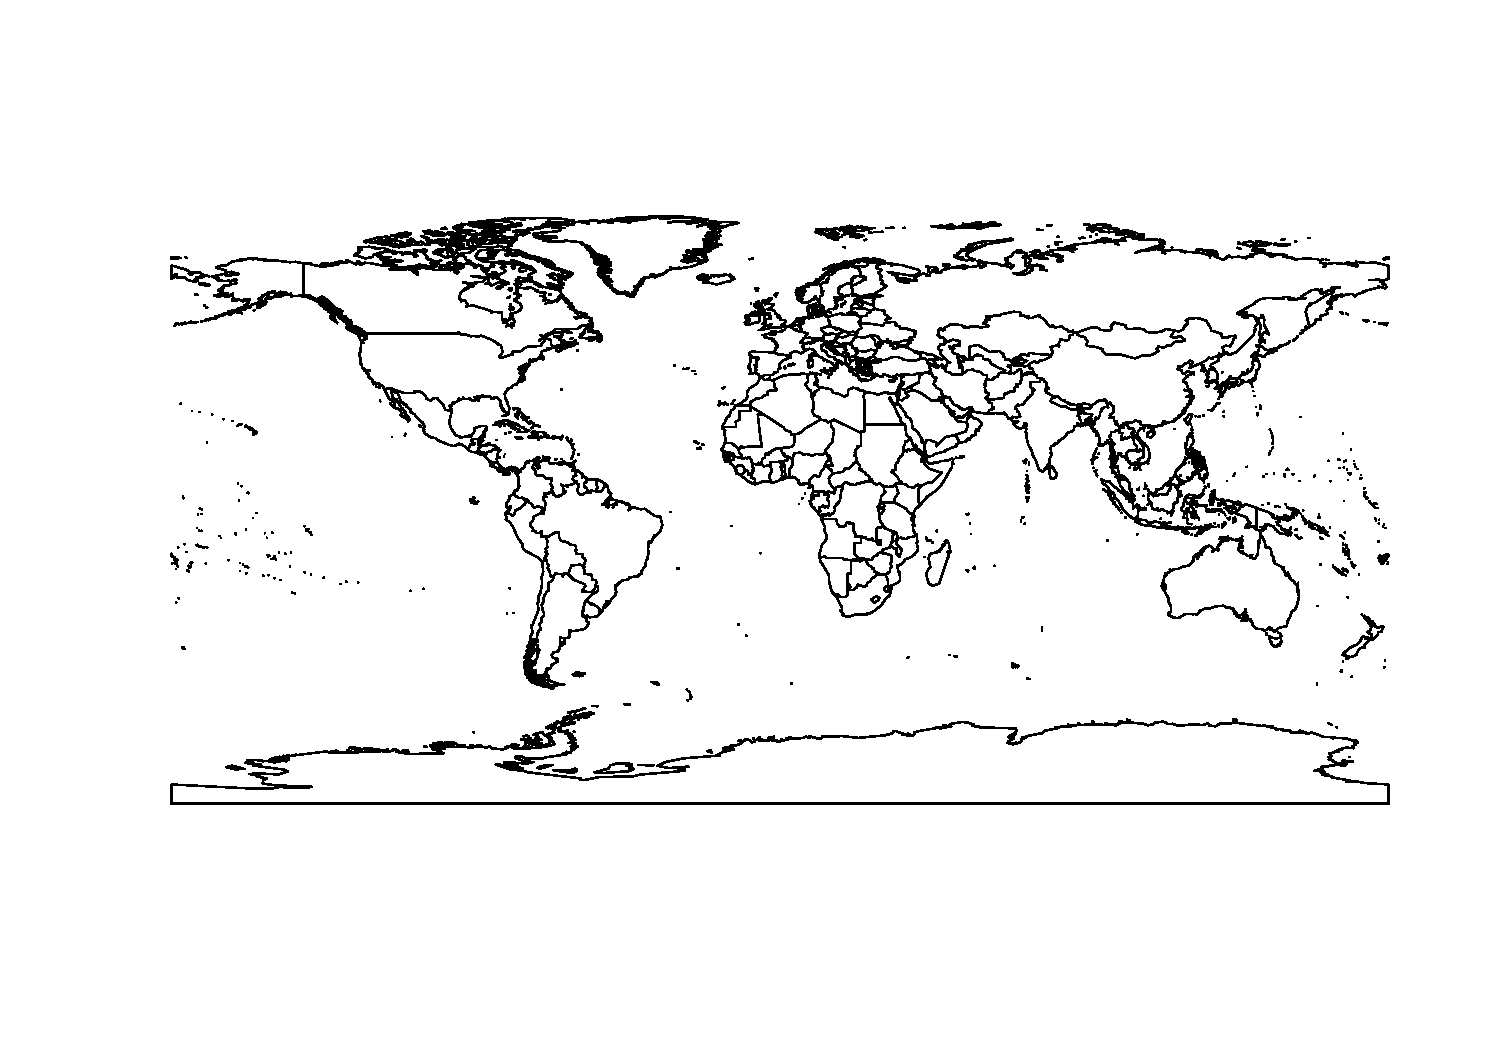
\includegraphics{Geomedizin_files/figure-beamer/unnamed-chunk-62-1.pdf}
=======
\begin{Shaded}
\begin{Highlighting}[]
\KeywordTok{library}\NormalTok{(}\StringTok{"RPostgreSQL"}\NormalTok{)}
\end{Highlighting}
\end{Shaded}

\end{block}

\end{frame}

\begin{frame}{Nutzung von Quantum GIS}

\begin{block}{\href{https://www.qgis.org/de/site/}{\textbf{QGIS}} - Ein
freies Open-Source-Geographisches-Informationssystem}

\begin{itemize}
\tightlist
\item
  Erstellen, bearbeiten, anzeigen, analysieren räumlicher Information
  unter Windows, Mac, Linux, BSD (bald auch Android)
\item
  Mit QGIS kann bspw auch der WMS/WCS oder WFS-Dienst des IÖR-Monitors
  genutzt werden.
\end{itemize}

\includegraphics{D:/Daten/GitHub/IntroR/buildingblocks/figure/Bilder_qgis.PNG})

\end{block}

\end{frame}

\begin{frame}{Nutze bspw. \href{http://www.qgis.org/de/site/}{QGIS} um
Shapefiles zu extrahieren}

\begin{itemize}
\tightlist
\item
  \href{http://www.qgistutorials.com/de/docs/downloading_osm_data.html}{Plugin
  OpenLayers}
\end{itemize}

\includegraphics{D:/Daten/GitHub/IntroR/buildingblocks/figure/stamen_watercolor1.png})

\end{frame}

\begin{frame}{Links}

\begin{itemize}
\item
  \href{http://wiki.openstreetmap.org/wiki/Downloading_data}{\textbf{Wiki
  zum Downlaod}} von Openstreetmap Daten
\item
  Auf dem \href{http://blog.openstreetmap.de/}{\textbf{Openstreetmap
  Blog}} gibt es wöchentlich neue Nachrichten zu OSM.
\item
  Liste möglicher Datenquellen für räumliche Analysen
  (\href{http://wiki.openstreetmap.org/wiki/Potential_Datasources}{weltweit}
  und in
  \href{http://wiki.openstreetmap.org/wiki/DE:Potential_Datasources}{\textbf{Deutschland}}
  )
\item
  Daten zu Administrative Grenzen kann man bei \emph{Second
  Administrative Level Boundaries}
  (\href{http://wiki.openstreetmap.org/wiki/SALB}{\textbf{SALB}})
  bekommen
\end{itemize}

\end{frame}

\section{Use Case Geomedizin}\label{use-case-geomedizin}

\begin{frame}{OpenStreetMap}

\includegraphics{D:/Daten/GitHub/IntroR/buildingblocks/figure/Openstreetmap_logo.svg.png}

\end{frame}

\begin{frame}{\href{https://wiki.openstreetmap.org/wiki/DE:Key:healthcare}{DE:Key:healthcare}}

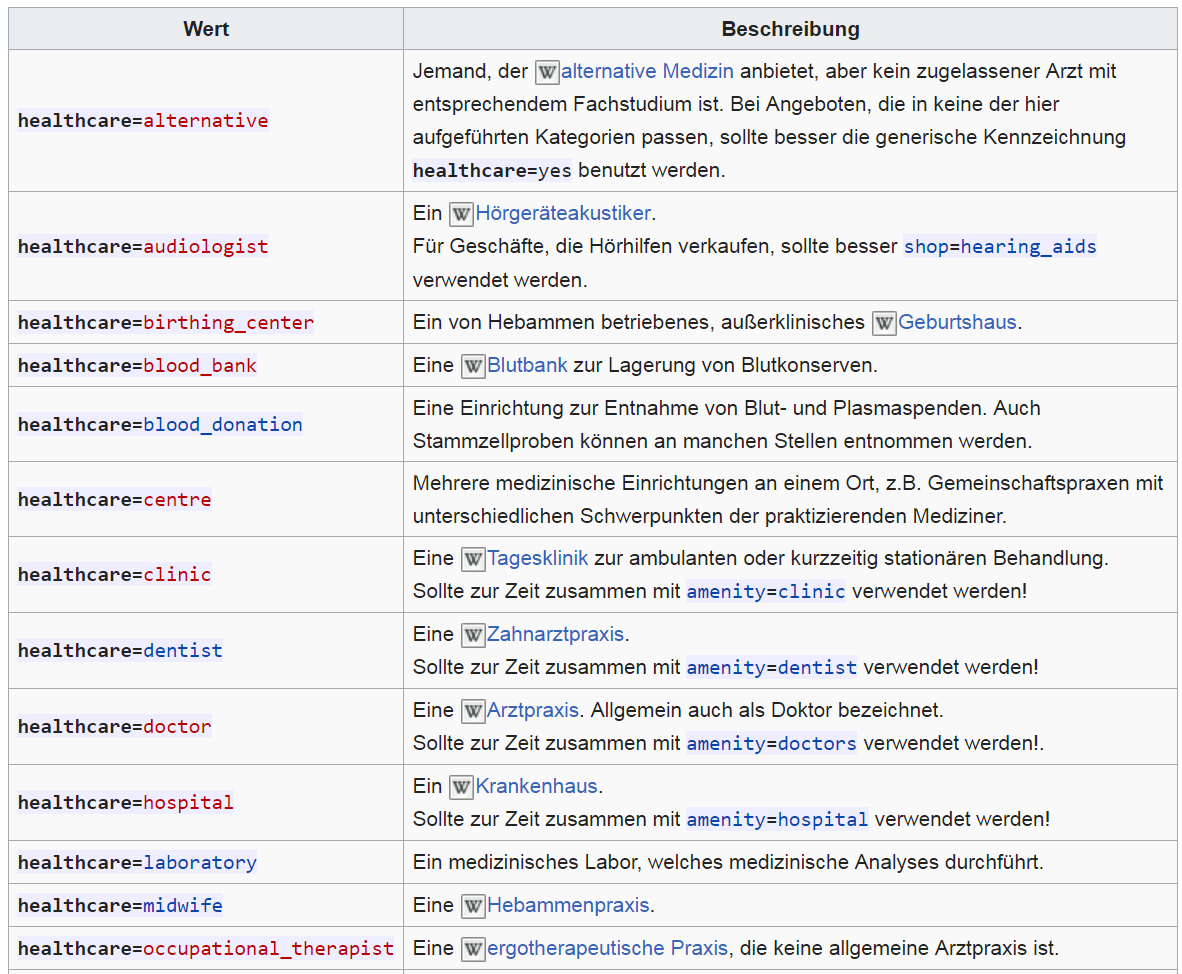
\includegraphics{D:/Daten/GitHub/IntroR/buildingblocks/figure/key_healthcare.PNG}

\end{frame}

\begin{frame}{Orte für die Blutspende}

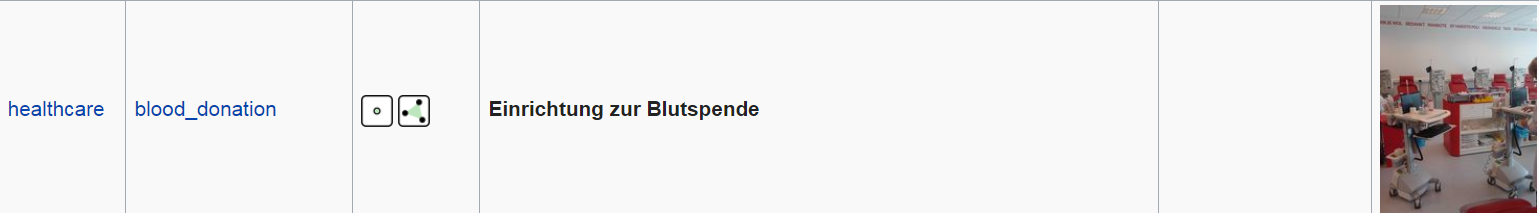
\includegraphics{D:/Daten/GitHub/IntroR/buildingblocks/figure/healthcare_blood_donation.PNG}

\end{frame}

\begin{frame}[fragile]{\href{https://overpass-turbo.eu/}{Die Nutzung von
Overpass}}

\begin{verbatim}
node
  [healthcare=blood_donation]
  ({{bbox}});
out;
\end{verbatim}

\end{frame}

\begin{frame}[fragile]{Alternativmediziner}

\begin{verbatim}
node
  [healthcare=alternative]
  ({{bbox}});
out;
\end{verbatim}

\end{frame}

\section{Erste Karten}\label{erste-karten}

\begin{frame}[fragile]{Das Paket maptools}

\begin{itemize}
\item
  Datensatz \texttt{wrld\_simpl} aus dem Paket
  \href{https://cran.r-project.org/web/packages/maptools/index.html}{maptools}
\item
  Polygone für fast alle Staaten der Erde

  \begin{longtable}[]{@{}rrrrrl@{}}
  \toprule
  FIPS & ISO2 & ISO3 & UN & NAME &\tabularnewline
  \midrule
  \endhead
  ATG & AC & AG & ATG & 28 & Antigua and Barbuda\tabularnewline
  DZA & AG & DZ & DZA & 12 & Algeria\tabularnewline
  AZE & AJ & AZ & AZE & 31 & Azerbaijan\tabularnewline
  ALB & AL & AL & ALB & 8 & Albania\tabularnewline
  \bottomrule
  \end{longtable}
\end{itemize}

\end{frame}

\begin{frame}{Hello world}


\includegraphics{Geomedizin_files/figure-beamer/unnamed-chunk-83-1.pdf}
>>>>>>> 01469a2fc21a4ee08106a146f700460dce05e2c7

\end{frame}

\begin{frame}[fragile]{Der shapefile}
\protect\hypertarget{der-shapefile}{}

\begin{itemize}
\tightlist
\item
  Es handelt sich um einen \texttt{shapefile}
\end{itemize}

\begin{verbatim}
## [1] "S4"
\end{verbatim}

\begin{itemize}
\tightlist
\item
  Die Daten sind als \texttt{S4} abgespeichert
\item
  Es gibt verschiedene Slots
\item
  In einem davon ist Information als \texttt{data.frame} gespeichert.
\end{itemize}

\end{frame}

<<<<<<< HEAD
\begin{frame}[fragile]{Der Datensatz}
\protect\hypertarget{der-datensatz}{}

\begin{Shaded}
\begin{Highlighting}[]
\KeywordTok{head}\NormalTok{(wrld_simpl}\OperatorTok{@}\NormalTok{data)}
\end{Highlighting}
\end{Shaded}
=======
\begin{frame}{Der Datensatz}
>>>>>>> 01469a2fc21a4ee08106a146f700460dce05e2c7

\begin{longtable}[]{@{}llllrl@{}}
\toprule
& FIPS & ISO2 & ISO3 & UN & NAME\tabularnewline
\midrule
\endhead
ATG & AC & AG & ATG & 28 & Antigua and Barbuda\tabularnewline
DZA & AG & DZ & DZA & 12 & Algeria\tabularnewline
AZE & AJ & AZ & AZE & 31 & Azerbaijan\tabularnewline
ALB & AL & AL & ALB & 8 & Albania\tabularnewline
\bottomrule
\end{longtable}

\end{frame}

\begin{frame}[fragile]{Die Struktur der Daten}
\protect\hypertarget{die-struktur-der-daten}{}

\begin{verbatim}
## [1] Antigua and Barbuda Algeria             Azerbaijan         
## [4] Albania             Armenia             Angola             
## 246 Levels: Aaland Islands Afghanistan Albania Algeria ... Zimbabwe
\end{verbatim}

\begin{verbatim}
## [1] AG DZ AZ AL AM AO
## 246 Levels: AD AE AF AG AI AL AM AN AO AQ AR AS AT AU AW AX AZ BA BB ... ZW
\end{verbatim}

\begin{verbatim}
## [1]    83039 32854159  8352021  3153731  3017661 16095214
\end{verbatim}

\end{frame}

\begin{frame}[fragile]{Eine logische Abfrage}
\protect\hypertarget{eine-logische-abfrage}{}

\begin{verbatim}
## [1] FALSE FALSE FALSE FALSE FALSE FALSE
\end{verbatim}

\begin{verbatim}
## ind_SA
## FALSE  TRUE 
##   245     1
\end{verbatim}

\end{frame}

<<<<<<< HEAD
\begin{frame}[fragile]{Eine Karte für Süd Afrika}
\protect\hypertarget{eine-karte-fur-sud-afrika}{}
=======
\begin{frame}{Eine Karte für Süd Afrika}
>>>>>>> 01469a2fc21a4ee08106a146f700460dce05e2c7

\begin{itemize}
\tightlist
\item
  Ein Land zeichnen
\end{itemize}

<<<<<<< HEAD
\begin{Shaded}
\begin{Highlighting}[]
\NormalTok{SouthAfrica <-}\StringTok{ }\NormalTok{wrld_simpl[ind_SA,]}
\KeywordTok{plot}\NormalTok{(SouthAfrica)}
\end{Highlighting}
\end{Shaded}


\includegraphics{Geomedizin_files/figure-beamer/unnamed-chunk-71-1.pdf}

\end{frame}

\begin{frame}[fragile]{Mehr als ein Land zeichnen}
\protect\hypertarget{mehr-als-ein-land-zeichnen}{}

\begin{Shaded}
\begin{Highlighting}[]
\NormalTok{EuropeList <-}\StringTok{ }\KeywordTok{c}\NormalTok{(}\StringTok{'Germany'}\NormalTok{, }\StringTok{'France'}\NormalTok{)}
\NormalTok{my_map <-}\StringTok{ }\NormalTok{wrld_simpl[wrld_simpl}\OperatorTok{$}\NormalTok{NAME }\OperatorTok\StringTok{ }\NormalTok{EuropeList, ]}
\KeywordTok{par}\NormalTok{(}\DataTypeTok{mai=}\KeywordTok{c}\NormalTok{(}\DecValTok{0}\NormalTok{,}\DecValTok{0}\NormalTok{,}\DecValTok{0}\NormalTok{,}\DecValTok{0}\NormalTok{))}
\KeywordTok{plot}\NormalTok{(my_map)}
\end{Highlighting}
\end{Shaded}

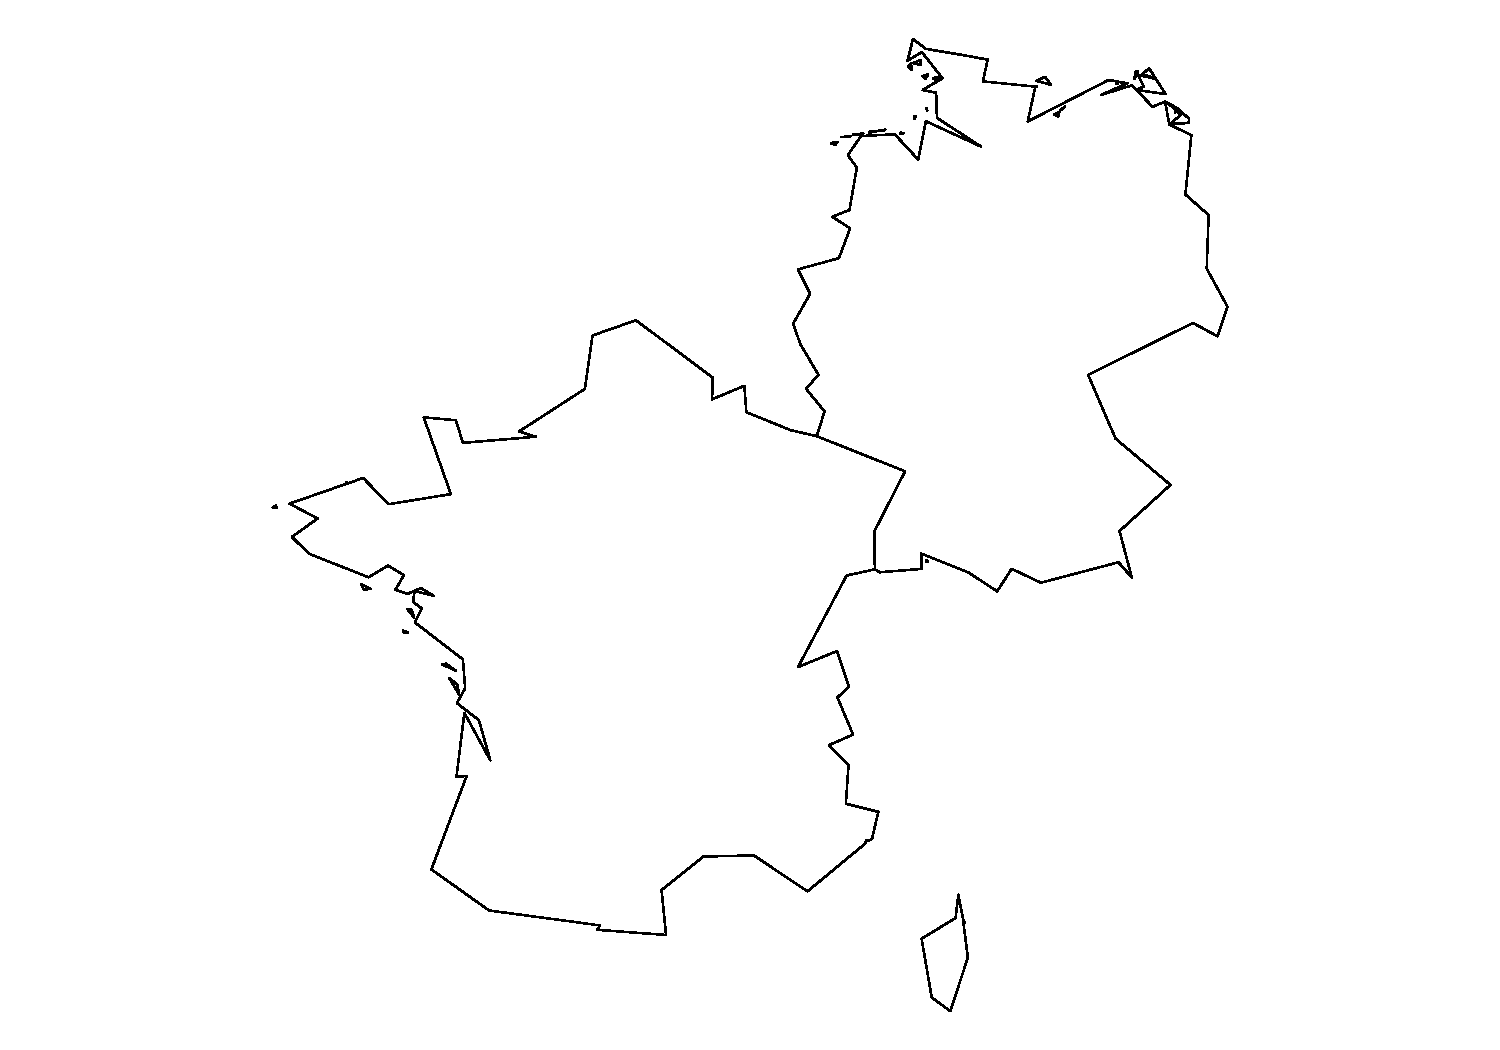
\includegraphics{Geomedizin_files/figure-beamer/unnamed-chunk-72-1.pdf}

\end{frame}

\begin{frame}[fragile]{Mehr Farbe}
\protect\hypertarget{mehr-farbe}{}

\begin{Shaded}
\begin{Highlighting}[]
\NormalTok{my_map}\OperatorTok{@}\NormalTok{data}\OperatorTok{$}\NormalTok{color <-}\StringTok{ }\KeywordTok{c}\NormalTok{(}\StringTok{"blue"}\NormalTok{,}\StringTok{"green"}\NormalTok{)}
\KeywordTok{plot}\NormalTok{(my_map,}\DataTypeTok{col=}\NormalTok{my_map}\OperatorTok{@}\NormalTok{data}\OperatorTok{$}\NormalTok{color)}
\end{Highlighting}
\end{Shaded}

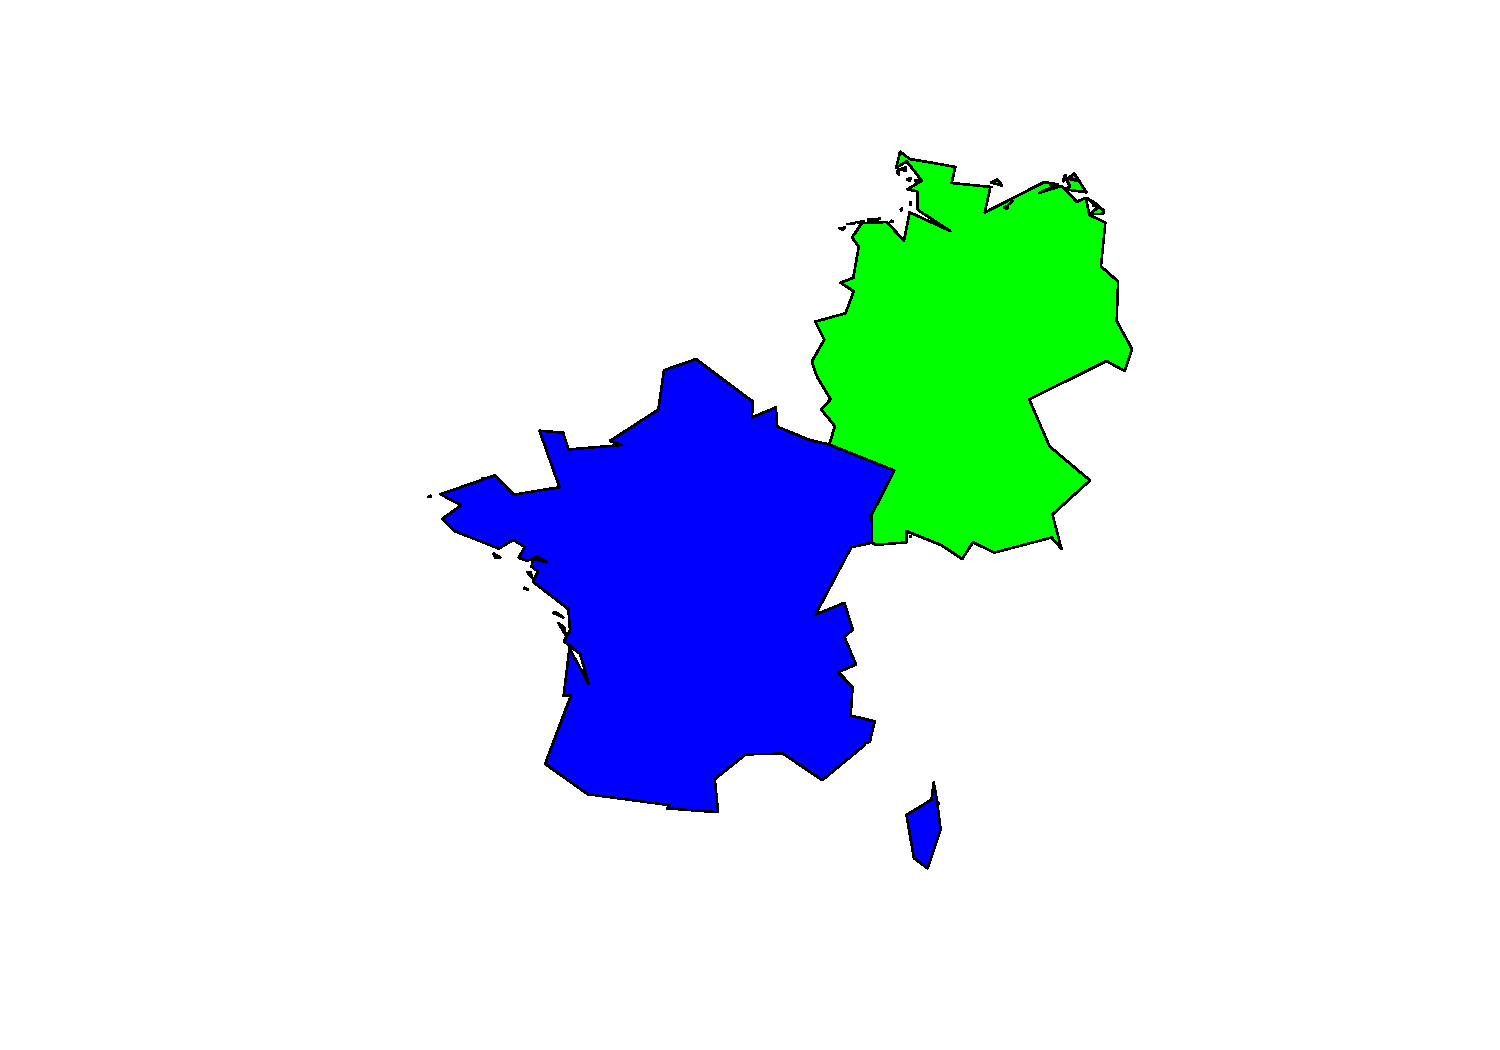
\includegraphics{Geomedizin_files/figure-beamer/unnamed-chunk-73-1.pdf}

\end{frame}

\begin{frame}[fragile]{Mehr Farbe für die Welt}
\protect\hypertarget{mehr-farbe-fur-die-welt}{}

\begin{Shaded}
\begin{Highlighting}[]
\KeywordTok{plot}\NormalTok{(wrld_simpl, }\DataTypeTok{bg=}\StringTok{'azure2'}\NormalTok{, }\DataTypeTok{col=}\StringTok{'green'}\NormalTok{,}
     \DataTypeTok{border=}\StringTok{'lightgray'}\NormalTok{)}
\end{Highlighting}
\end{Shaded}

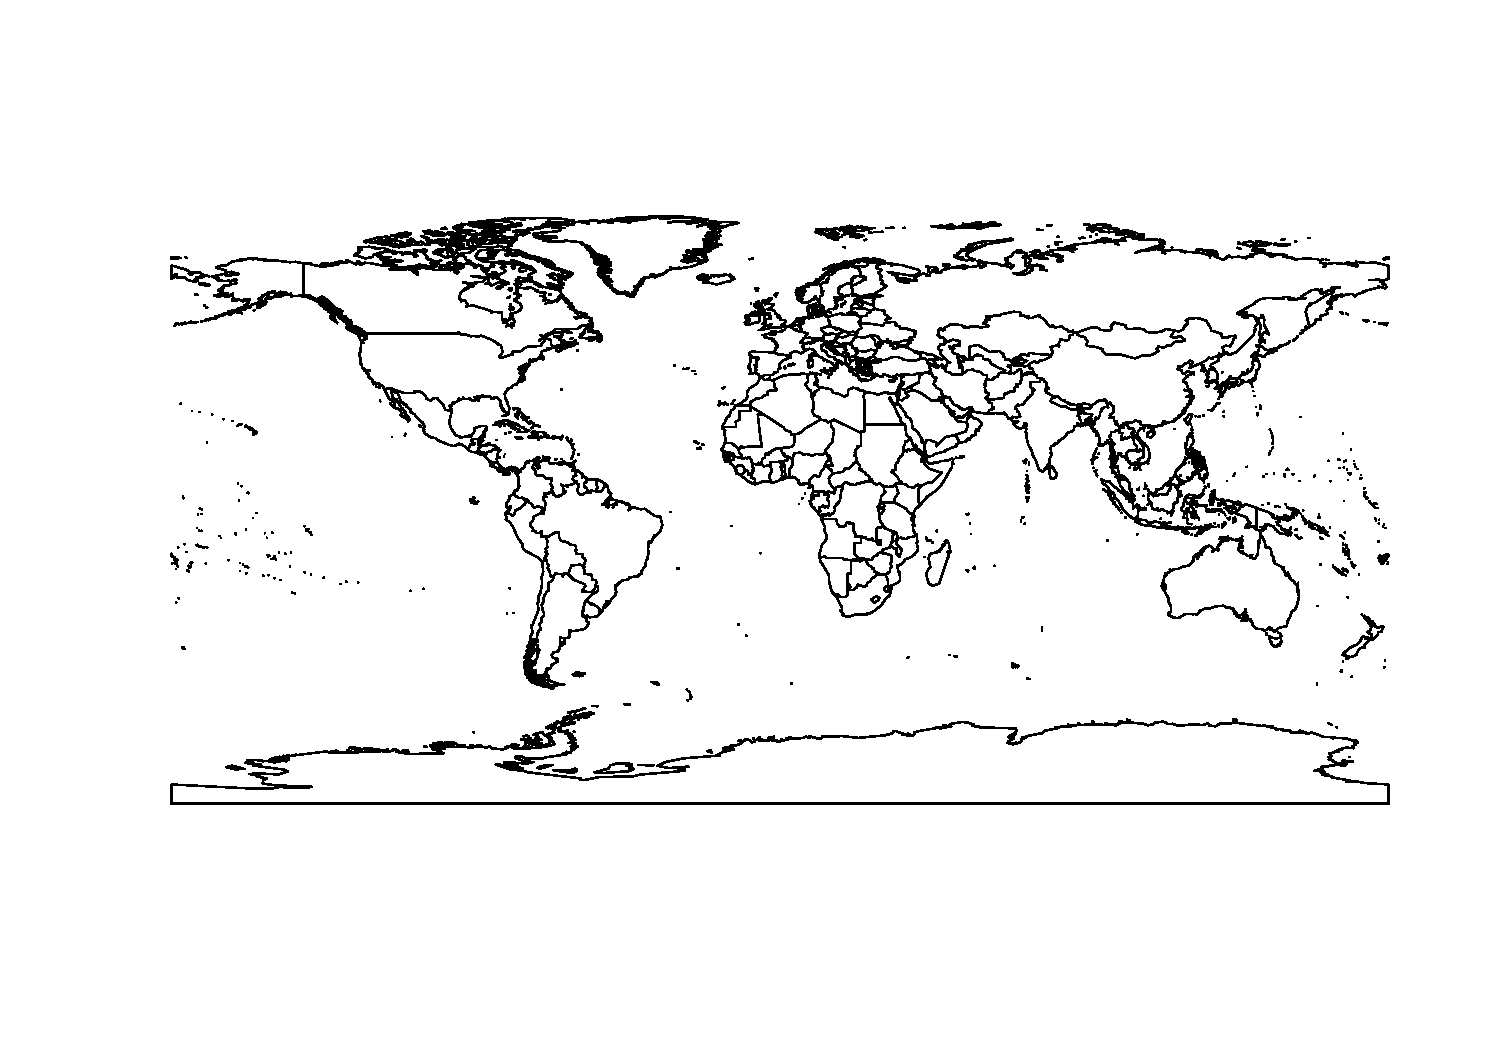
\includegraphics{Geomedizin_files/figure-beamer/unnamed-chunk-74-1.pdf}

\end{frame}

\begin{frame}[fragile]{Eine Karte für Europa}
\protect\hypertarget{eine-karte-fur-europa}{}

\begin{Shaded}
\begin{Highlighting}[]
\NormalTok{Europe <-}\StringTok{ }\NormalTok{wrld_simpl[wrld_simpl}\OperatorTok{$}\NormalTok{REGION}\OperatorTok{==}\StringTok{"150"}\NormalTok{,]}
\KeywordTok{plot}\NormalTok{(Europe,}\DataTypeTok{col=}\StringTok{"royalblue"}\NormalTok{)}
\end{Highlighting}
\end{Shaded}

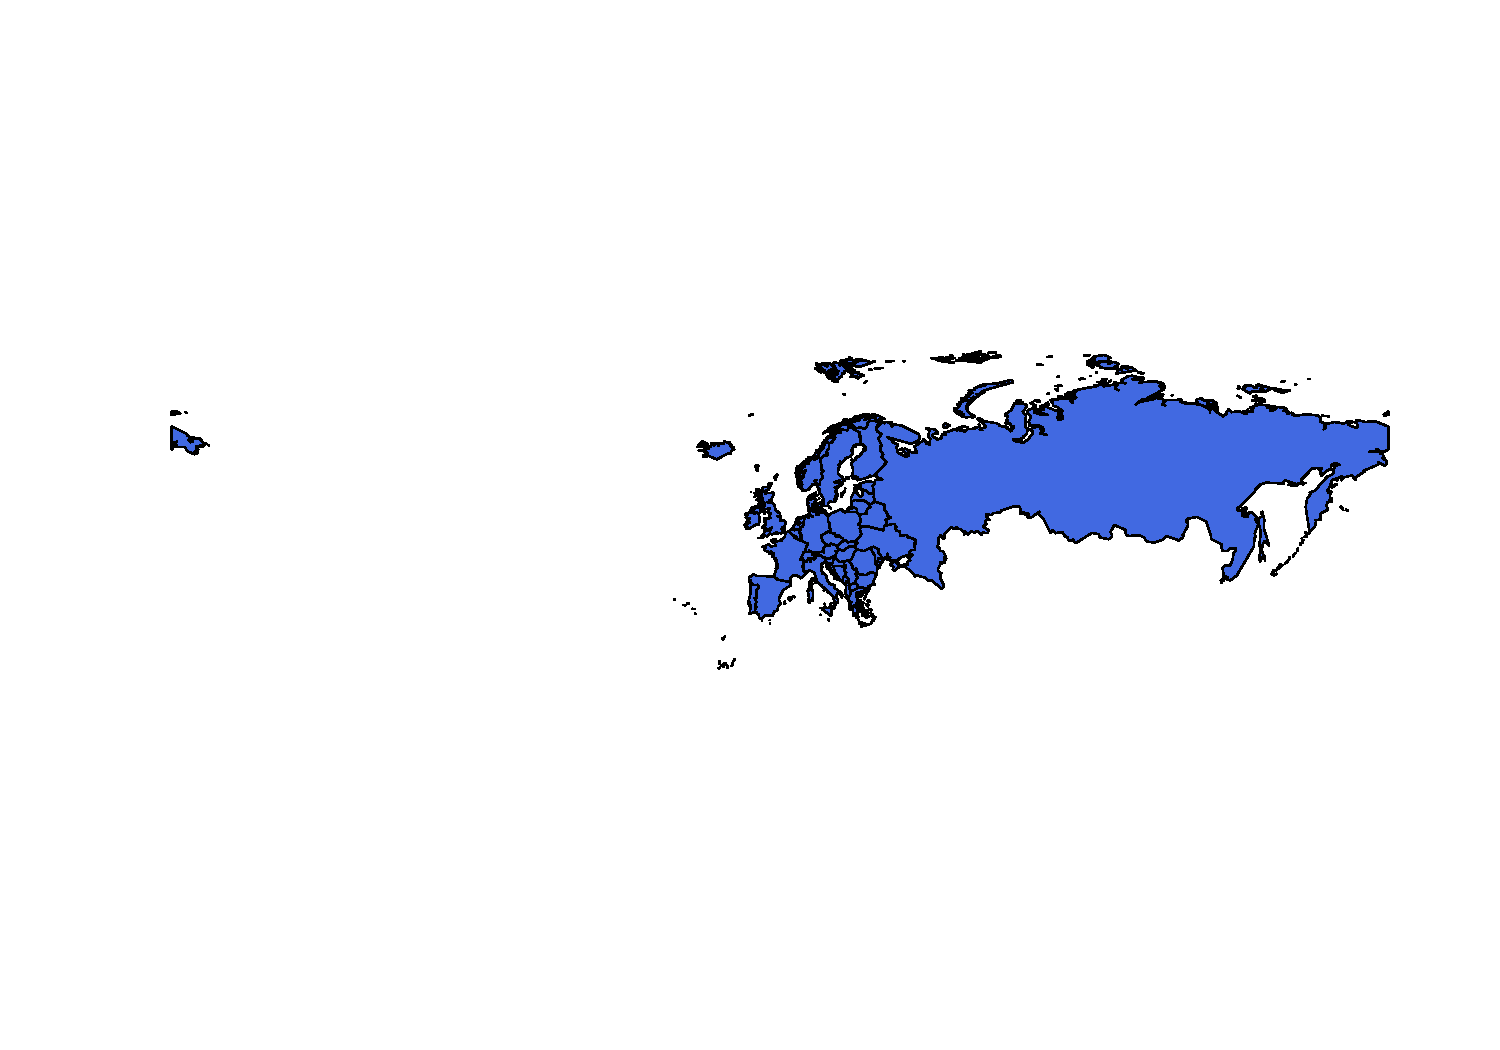
\includegraphics{Geomedizin_files/figure-beamer/unnamed-chunk-75-1.pdf}

\end{frame}

\begin{frame}[fragile]{Europa ohne Russland}
\protect\hypertarget{europa-ohne-russland}{}

\begin{Shaded}
\begin{Highlighting}[]
\NormalTok{ind <-}\StringTok{ }\KeywordTok{which}\NormalTok{(Europe}\OperatorTok{@}\NormalTok{data}\OperatorTok{$}\NormalTok{NAME}\OperatorTok{==}\StringTok{"Russia"}\NormalTok{)}
\NormalTok{EU <-}\StringTok{ }\NormalTok{Europe[}\OperatorTok{-}\NormalTok{ind,]}
\KeywordTok{plot}\NormalTok{(EU,}\DataTypeTok{col=}\StringTok{"blue"}\NormalTok{,}\DataTypeTok{border=}\StringTok{"darkgray"}\NormalTok{)}
\end{Highlighting}
\end{Shaded}

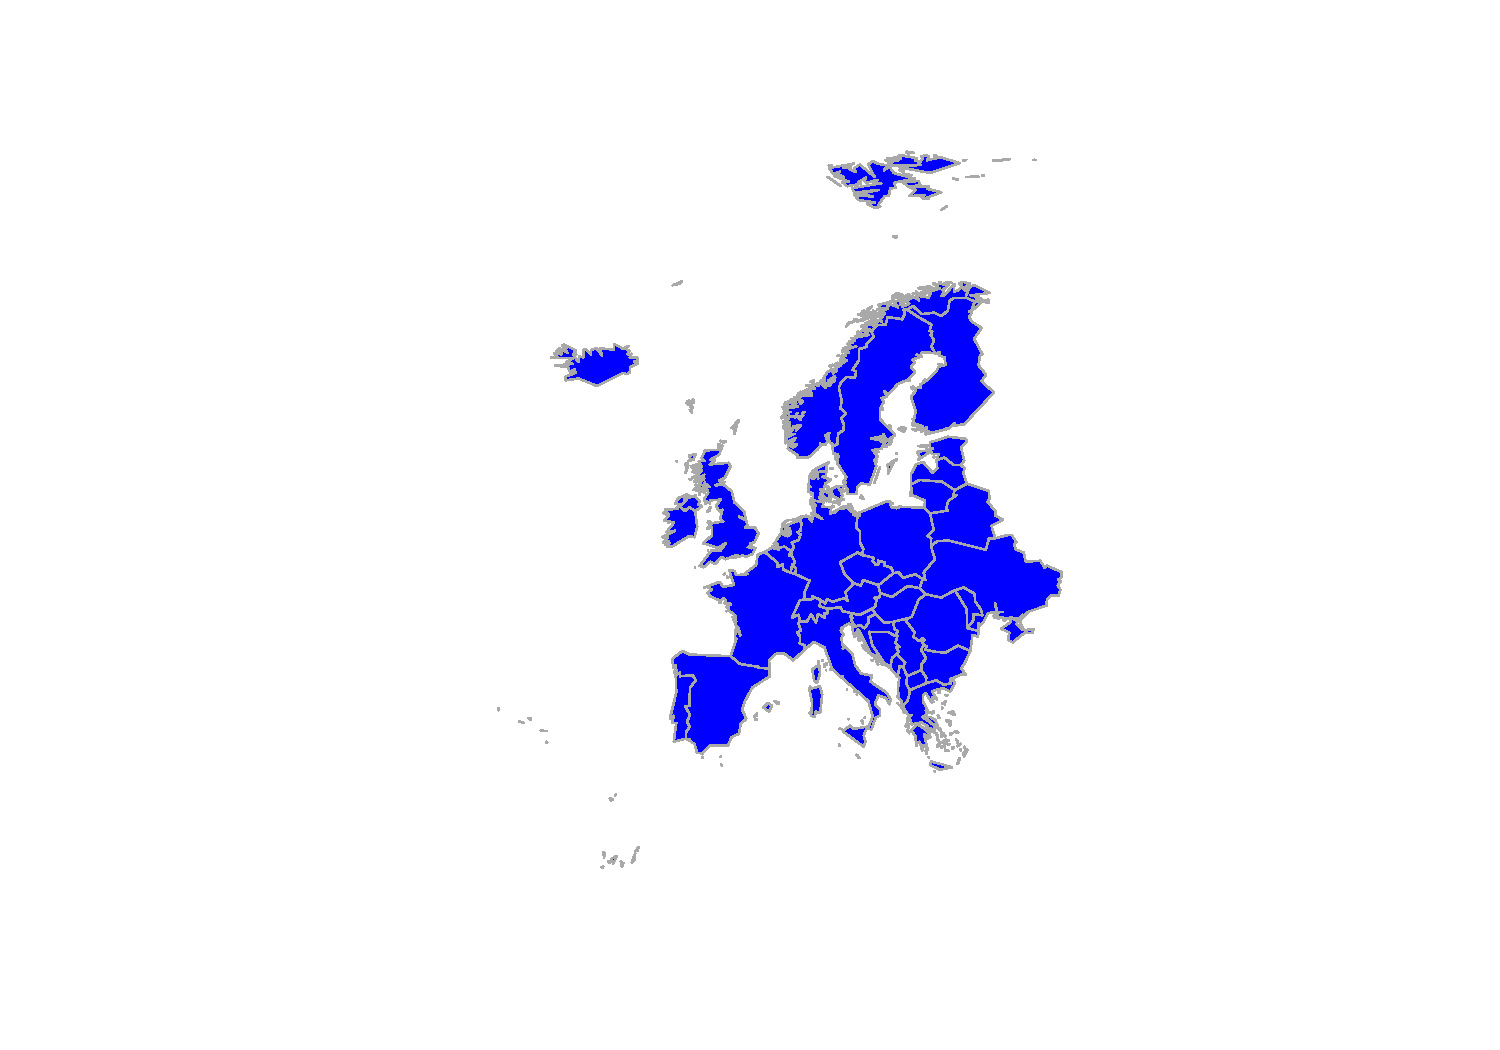
\includegraphics{Geomedizin_files/figure-beamer/unnamed-chunk-76-1.pdf}

\end{frame}

\begin{frame}[fragile]{Spielen Sie mit Farben}
\protect\hypertarget{spielen-sie-mit-farben}{}

\begin{Shaded}
\begin{Highlighting}[]
\NormalTok{EU}\OperatorTok{$}\NormalTok{colors <-}\StringTok{ "green"}
\KeywordTok{plot}\NormalTok{(EU,}\DataTypeTok{col=}\NormalTok{EU}\OperatorTok{$}\NormalTok{colors,}\DataTypeTok{border=}\StringTok{"darkgray"}\NormalTok{)}
\end{Highlighting}
\end{Shaded}

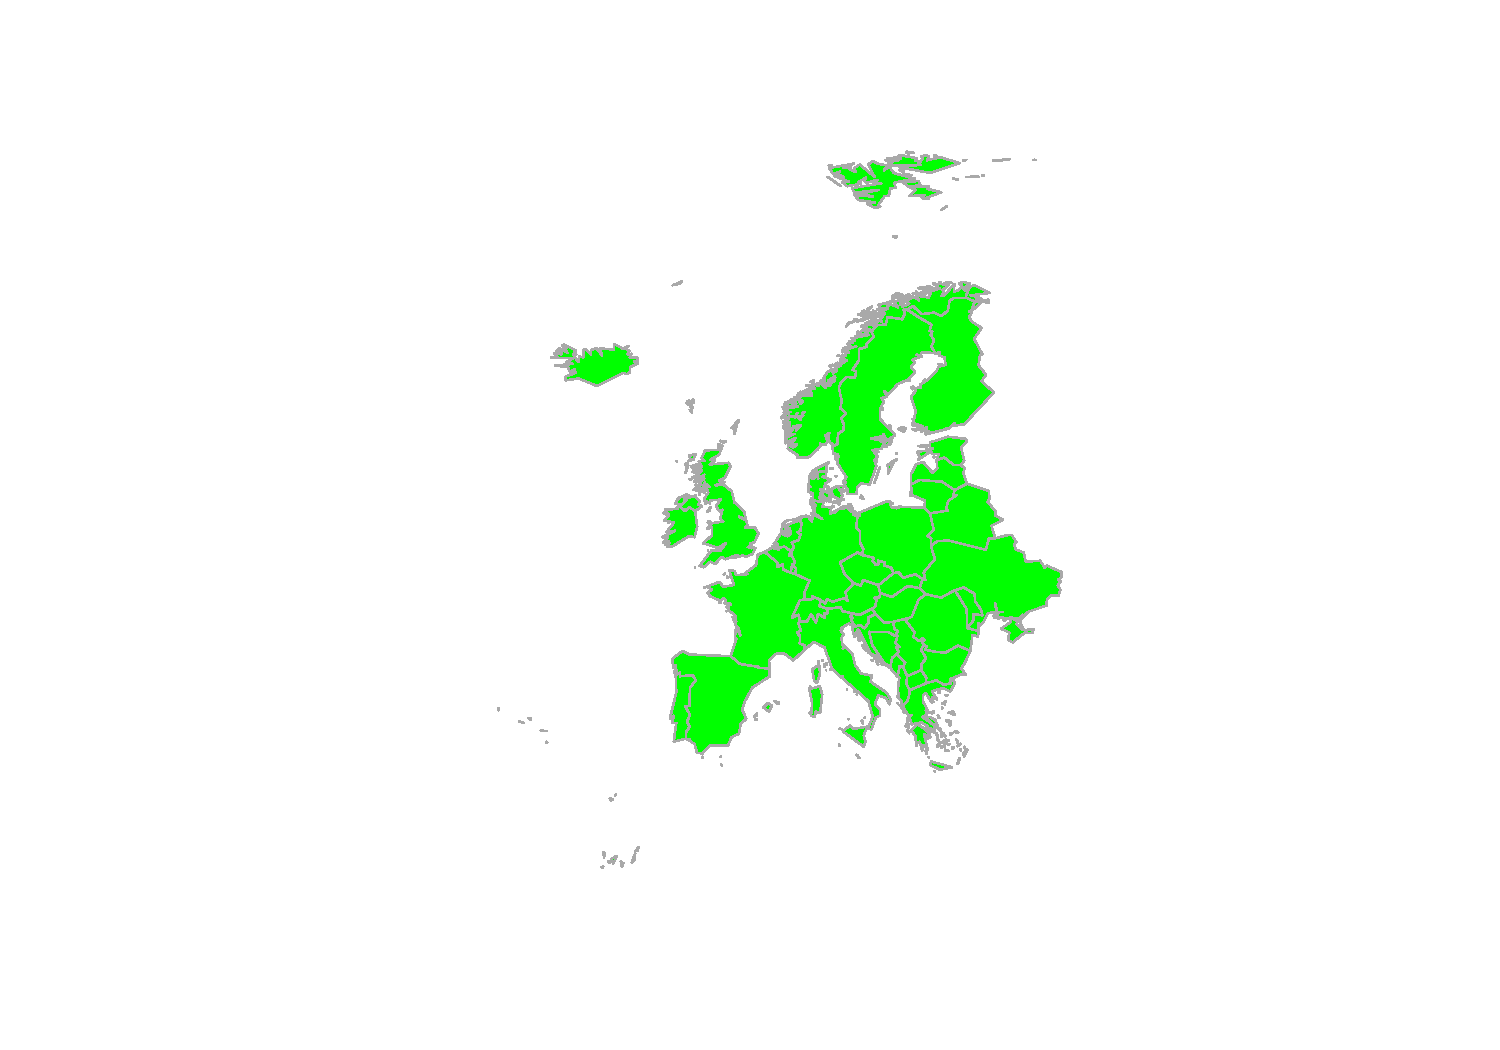
\includegraphics{Geomedizin_files/figure-beamer/unnamed-chunk-77-1.pdf}

\begin{Shaded}
\begin{Highlighting}[]
\NormalTok{pop05 <-}\StringTok{ }\NormalTok{Europe}\OperatorTok{$}\NormalTok{POP2005}
\NormalTok{Europe}\OperatorTok{$}\NormalTok{colors[pop05}\OperatorTok{>}\KeywordTok{mean}\NormalTok{(pop05)] <-}\StringTok{ "royalblue"}
\KeywordTok{plot}\NormalTok{(Europe,}\DataTypeTok{col=}\NormalTok{Europe}\OperatorTok{$}\NormalTok{colors)}
\end{Highlighting}
\end{Shaded}

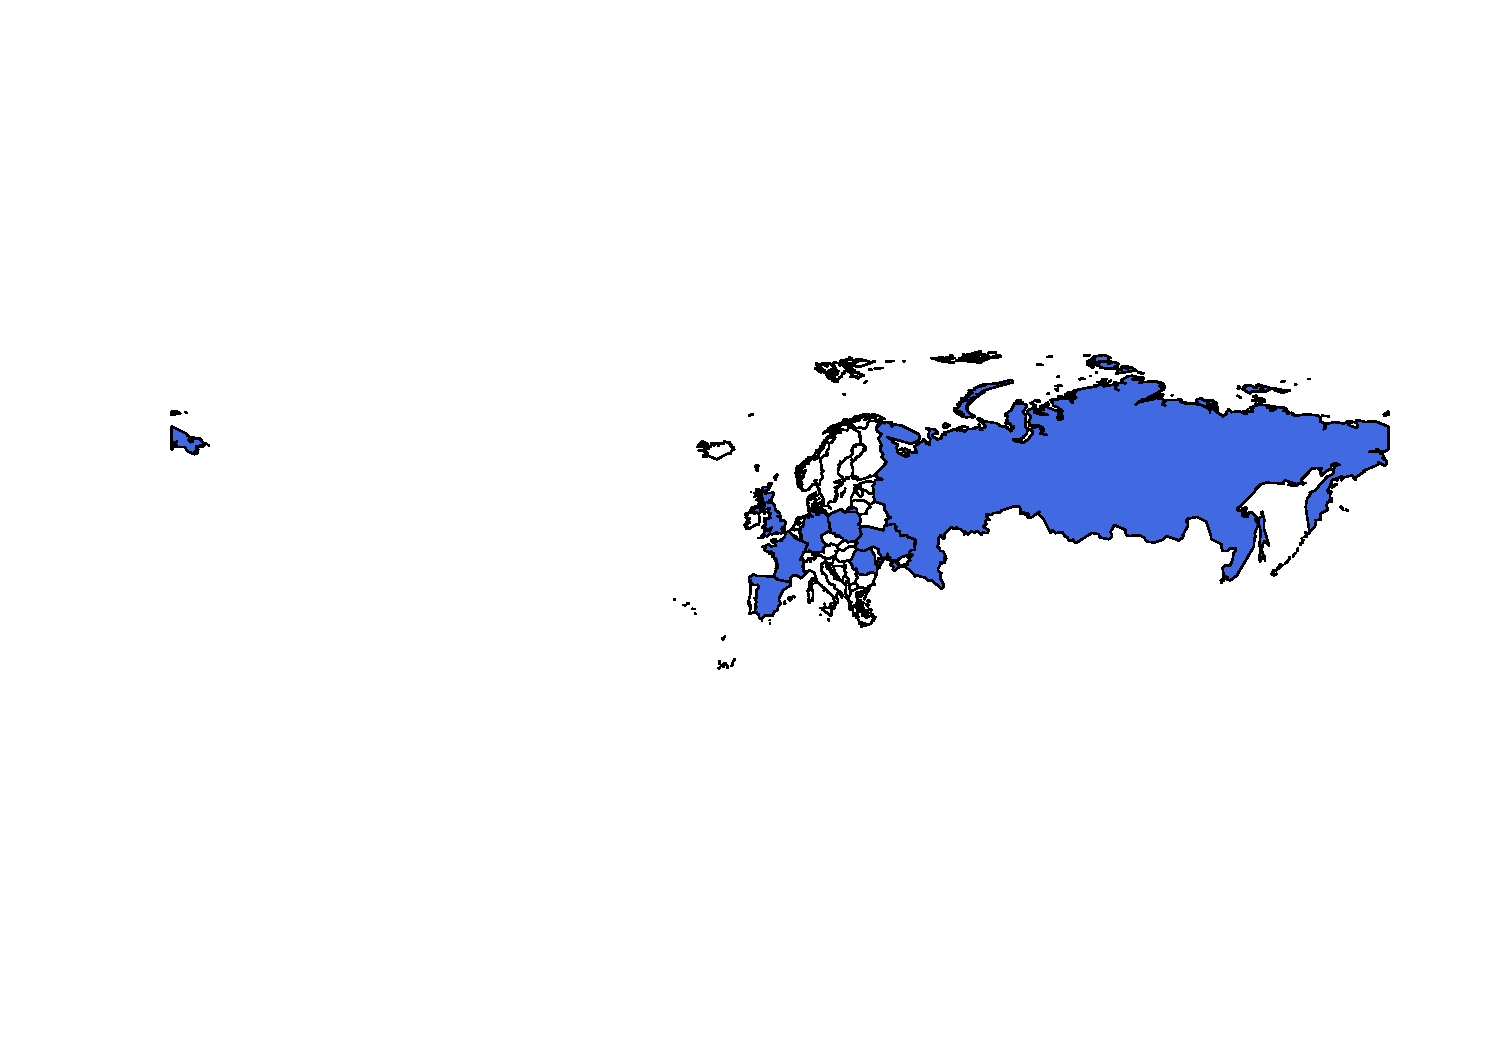
\includegraphics{Geomedizin_files/figure-beamer/unnamed-chunk-77-2.pdf}

\end{frame}

\begin{frame}[fragile]{Mehr über Farben}
\protect\hypertarget{mehr-uber-farben}{}
=======

\includegraphics{Geomedizin_files/figure-beamer/unnamed-chunk-92-1.pdf}

\end{frame}

\begin{frame}{Mehr als ein Land zeichnen}

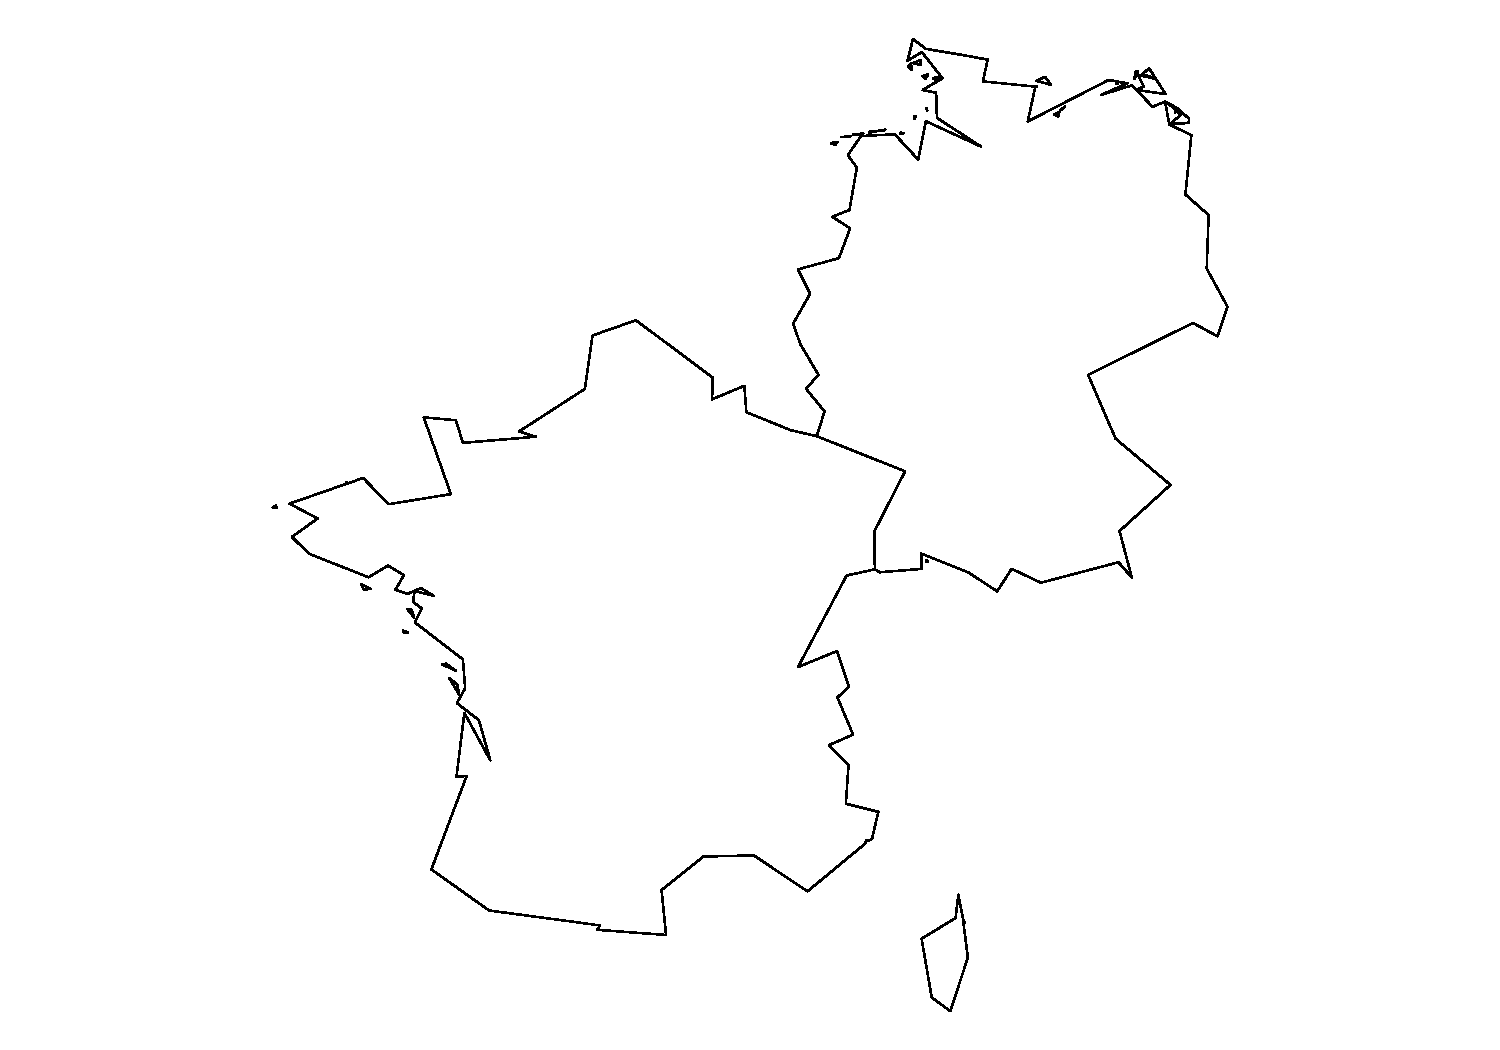
\includegraphics{Geomedizin_files/figure-beamer/unnamed-chunk-93-1.pdf}

\end{frame}

\begin{frame}{Mehr Farbe}

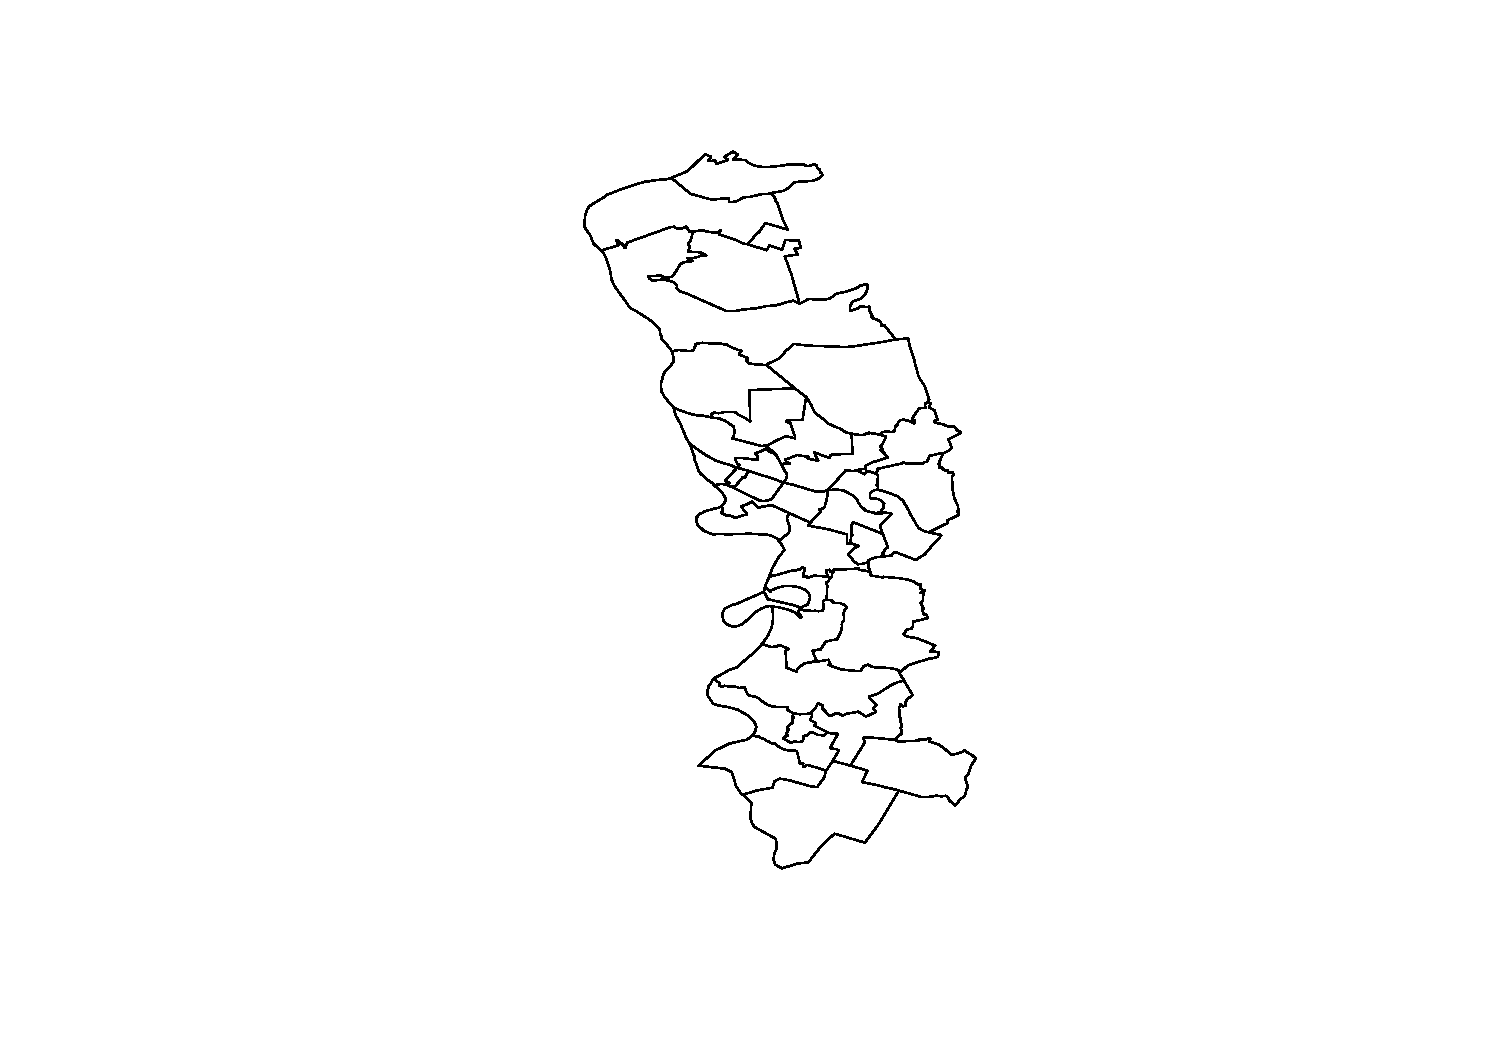
\includegraphics{Geomedizin_files/figure-beamer/unnamed-chunk-94-1.pdf}

\end{frame}

\begin{frame}{Mehr Farbe für die Welt}

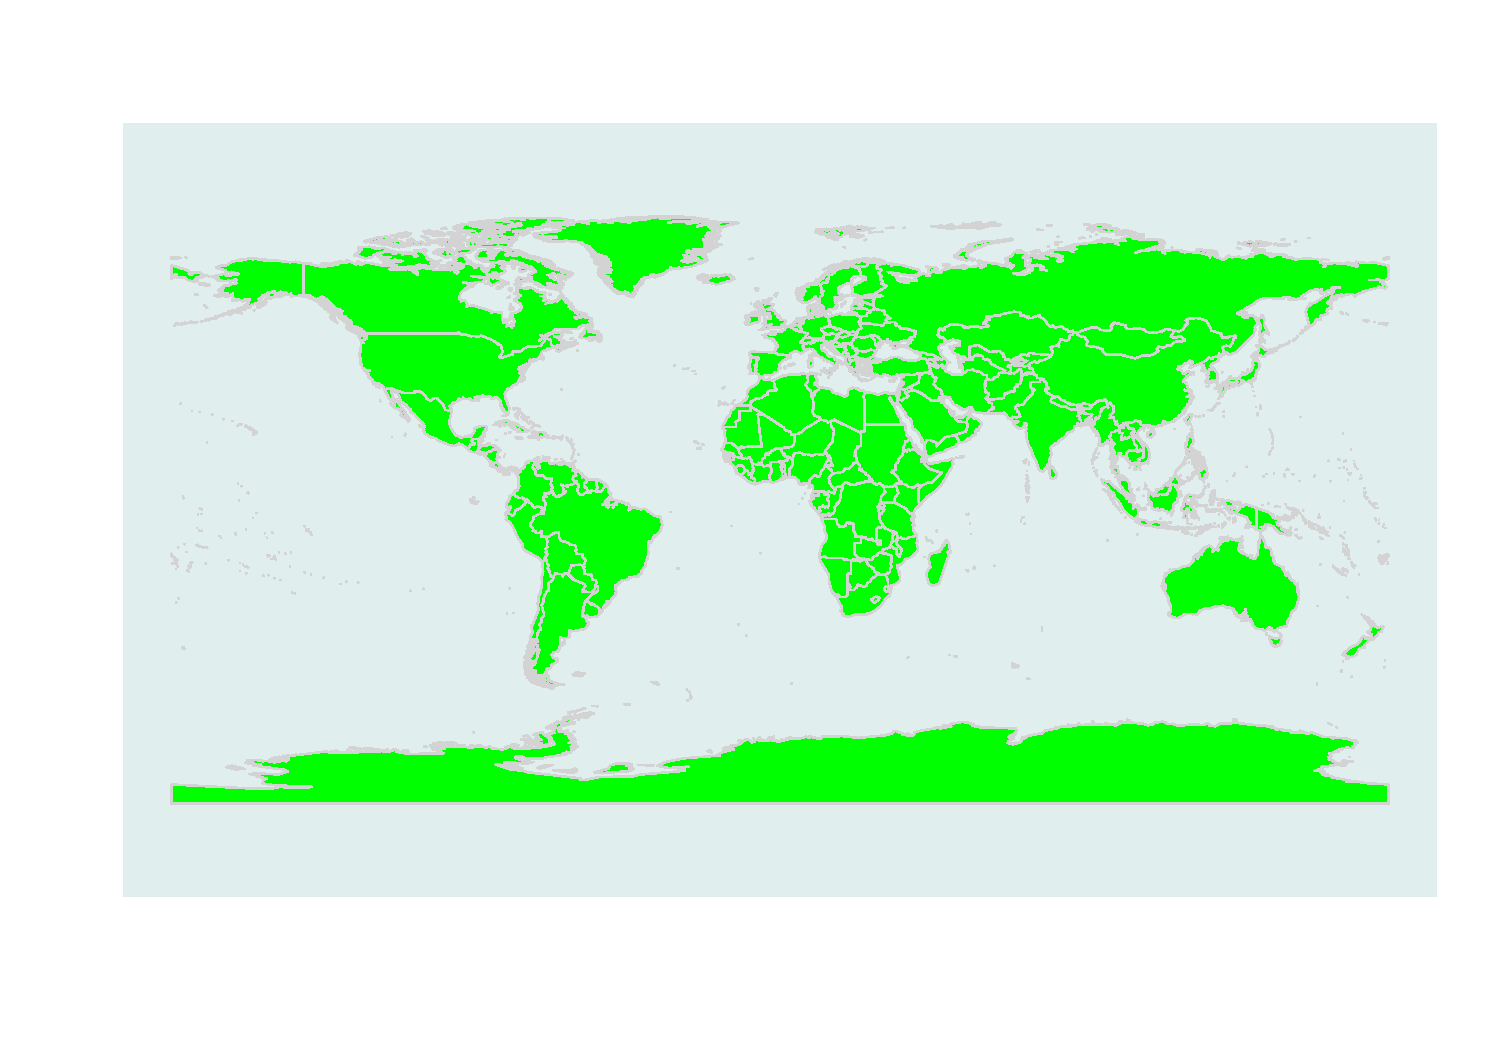
\includegraphics{Geomedizin_files/figure-beamer/unnamed-chunk-95-1.pdf}

\end{frame}

\begin{frame}{Eine Karte für Europa}


\includegraphics{Geomedizin_files/figure-beamer/unnamed-chunk-96-1.pdf}

\end{frame}

\begin{frame}{Europa ohne Russland}

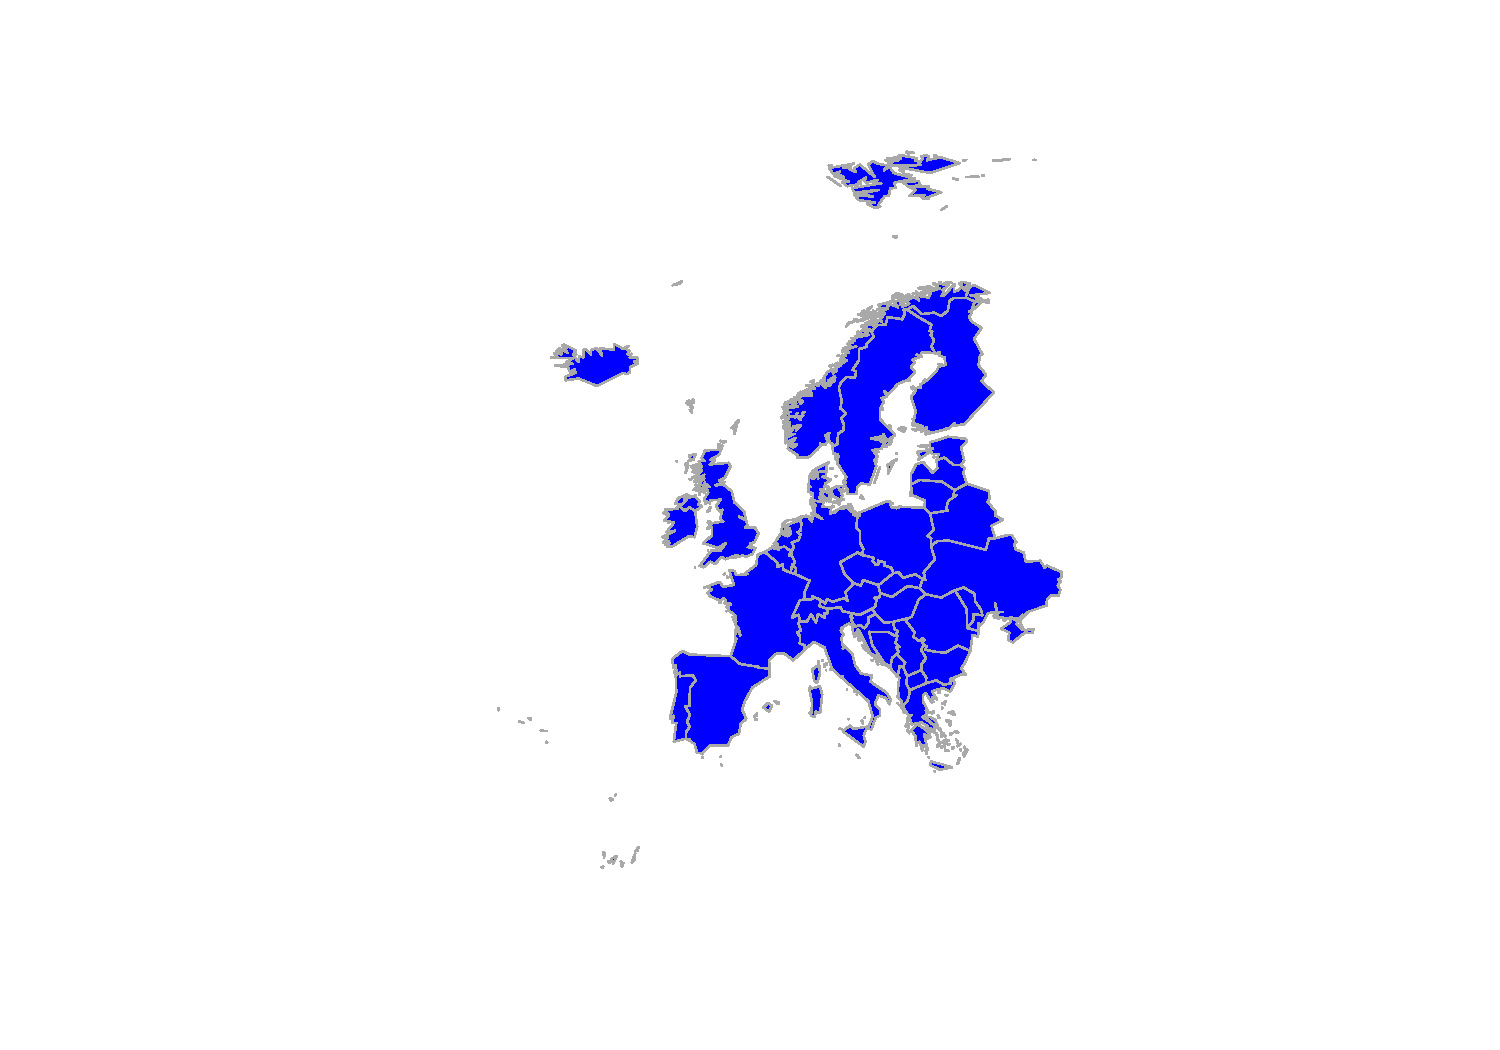
\includegraphics{Geomedizin_files/figure-beamer/unnamed-chunk-97-1.pdf}

\end{frame}

\begin{frame}{Spielen Sie mit Farben}

\includegraphics{Geomedizin_files/figure-beamer/unnamed-chunk-98-1.pdf}
\includegraphics{Geomedizin_files/figure-beamer/unnamed-chunk-98-2.pdf}

\end{frame}

\begin{frame}{Mehr über Farben}
>>>>>>> 01469a2fc21a4ee08106a146f700460dce05e2c7

\href{http://www.stat.columbia.edu/~tzheng/files/Rcolor.pdf}{Colors in
R}

<<<<<<< HEAD
\begin{Shaded}
\begin{Highlighting}[]
\NormalTok{Europe}\OperatorTok{$}\NormalTok{colors[pop05}\OperatorTok{>}\KeywordTok{median}\NormalTok{(pop05)] <-}\StringTok{ "chocolate4"}
\KeywordTok{plot}\NormalTok{(Europe,}\DataTypeTok{col=}\NormalTok{Europe}\OperatorTok{$}\NormalTok{colors)}
\end{Highlighting}
\end{Shaded}

\includegraphics{Geomedizin_files/figure-beamer/unnamed-chunk-78-1.pdf}

\end{frame}

\begin{frame}[fragile]{Europa - Farbschattierung blau}
\protect\hypertarget{europa---farbschattierung-blau}{}

\begin{Shaded}
\begin{Highlighting}[]
\NormalTok{val <-}\StringTok{ }\NormalTok{Europe}\OperatorTok{$}\NormalTok{POP2005}\OperatorTok{/}\KeywordTok{max}\NormalTok{(Europe}\OperatorTok{$}\NormalTok{POP2005)}
\KeywordTok{plot}\NormalTok{(Europe,}\DataTypeTok{col=}\KeywordTok{rgb}\NormalTok{(}\DecValTok{0}\NormalTok{,}\DecValTok{0}\NormalTok{,val))}
\end{Highlighting}
\end{Shaded}

\includegraphics{Geomedizin_files/figure-beamer/unnamed-chunk-79-1.pdf}

\end{frame}

\begin{frame}[fragile]{Europa - Farbschattierung rot}
\protect\hypertarget{europa---farbschattierung-rot}{}

\begin{Shaded}
\begin{Highlighting}[]
\NormalTok{val <-}\StringTok{ }\NormalTok{Europe}\OperatorTok{$}\NormalTok{POP2005}\OperatorTok{/}\KeywordTok{max}\NormalTok{(Europe}\OperatorTok{$}\NormalTok{POP2005)}
\KeywordTok{plot}\NormalTok{(Europe,}\DataTypeTok{col=}\KeywordTok{rgb}\NormalTok{(val,}\DecValTok{0}\NormalTok{,}\DecValTok{0}\NormalTok{))}
\end{Highlighting}
\end{Shaded}

\includegraphics{Geomedizin_files/figure-beamer/unnamed-chunk-80-1.pdf}

\end{frame}

\begin{frame}[fragile]{Europa - Farbschattierung grün}
\protect\hypertarget{europa---farbschattierung-grun}{}

\begin{Shaded}
\begin{Highlighting}[]
\NormalTok{val <-}\StringTok{ }\NormalTok{Europe}\OperatorTok{$}\NormalTok{POP2005}\OperatorTok{/}\KeywordTok{max}\NormalTok{(Europe}\OperatorTok{$}\NormalTok{POP2005)}
\KeywordTok{plot}\NormalTok{(Europe,}\DataTypeTok{col=}\KeywordTok{rgb}\NormalTok{(}\DecValTok{0}\NormalTok{,val,}\DecValTok{0}\NormalTok{))}
\end{Highlighting}
\end{Shaded}

\includegraphics{Geomedizin_files/figure-beamer/unnamed-chunk-81-1.pdf}

\end{frame}

\begin{frame}[fragile]{Europa - Farbschattierung grau}
\protect\hypertarget{europa---farbschattierung-grau}{}

\begin{Shaded}
\begin{Highlighting}[]
\NormalTok{val <-}\StringTok{ }\NormalTok{Europe}\OperatorTok{$}\NormalTok{POP2005}\OperatorTok{/}\KeywordTok{max}\NormalTok{(Europe}\OperatorTok{$}\NormalTok{POP2005)}
\KeywordTok{plot}\NormalTok{(Europe,}\DataTypeTok{col=}\KeywordTok{rgb}\NormalTok{(val,val,val))}
\end{Highlighting}
\end{Shaded}

\includegraphics{Geomedizin_files/figure-beamer/unnamed-chunk-82-1.pdf}

\end{frame}

\begin{frame}[fragile]{Europa - zwei Graphiken nebeneinander}
\protect\hypertarget{europa---zwei-graphiken-nebeneinander}{}

\begin{Shaded}
\begin{Highlighting}[]
\KeywordTok{par}\NormalTok{(}\DataTypeTok{mfrow=}\KeywordTok{c}\NormalTok{(}\DecValTok{1}\NormalTok{,}\DecValTok{2}\NormalTok{))}
\KeywordTok{plot}\NormalTok{(Europe,}\DataTypeTok{col=}\KeywordTok{rgb}\NormalTok{(val,}\DecValTok{0}\NormalTok{,val))}
\KeywordTok{plot}\NormalTok{(Europe,}\DataTypeTok{col=}\KeywordTok{rgb}\NormalTok{(val,val,}\DecValTok{0}\NormalTok{))}
\end{Highlighting}
\end{Shaded}

\includegraphics{Geomedizin_files/figure-beamer/unnamed-chunk-83-1.pdf}
=======
\includegraphics{Geomedizin_files/figure-beamer/unnamed-chunk-99-1.pdf}

\end{frame}

\begin{frame}{Europa - Farbschattierung blau}

\includegraphics{Geomedizin_files/figure-beamer/unnamed-chunk-100-1.pdf}

\end{frame}

\begin{frame}{Europa - Farbschattierung rot}

\includegraphics{Geomedizin_files/figure-beamer/unnamed-chunk-101-1.pdf}

\end{frame}

\begin{frame}{Europa - Farbschattierung grün}

\includegraphics{Geomedizin_files/figure-beamer/unnamed-chunk-102-1.pdf}

\end{frame}

\begin{frame}{Europa - Farbschattierung grau}

\includegraphics{Geomedizin_files/figure-beamer/unnamed-chunk-103-1.pdf}

\end{frame}

\begin{frame}{Europa - zwei Graphiken nebeneinander}

\includegraphics{Geomedizin_files/figure-beamer/unnamed-chunk-104-1.pdf}
>>>>>>> 01469a2fc21a4ee08106a146f700460dce05e2c7

\end{frame}

\begin{frame}[fragile]{Europa - Punkte hinzufügen}
\protect\hypertarget{europa---punkte-hinzufugen}{}

\begin{verbatim}
## [1] 10
\end{verbatim}

<<<<<<< HEAD
\begin{Shaded}
\begin{Highlighting}[]
\KeywordTok{plot}\NormalTok{(Europe)}
\KeywordTok{points}\NormalTok{(Europe}\OperatorTok{$}\NormalTok{LON[}\DecValTok{10}\NormalTok{],Europe}\OperatorTok{$}\NormalTok{LAT[}\DecValTok{10}\NormalTok{],}\DataTypeTok{col=}\StringTok{"red"}\NormalTok{,}\DataTypeTok{pch=}\DecValTok{20}\NormalTok{)}
\end{Highlighting}
\end{Shaded}

\includegraphics{Geomedizin_files/figure-beamer/unnamed-chunk-84-1.pdf}

\end{frame}

\begin{frame}[fragile]{Europa - Blasen hinzufügen}
\protect\hypertarget{europa---blasen-hinzufugen}{}

\begin{Shaded}
\begin{Highlighting}[]
\NormalTok{pop <-}\StringTok{ }\NormalTok{Europe}\OperatorTok{$}\NormalTok{POP2005}
\NormalTok{pop <-}\StringTok{ }\NormalTok{pop}\OperatorTok{/}\KeywordTok{max}\NormalTok{(pop)}\OperatorTok{*}\DecValTok{10}
\KeywordTok{plot}\NormalTok{(Europe)}
\KeywordTok{points}\NormalTok{(Europe}\OperatorTok{$}\NormalTok{LON,Europe}\OperatorTok{$}\NormalTok{LAT,}\DataTypeTok{cex=}\NormalTok{pop,}\DataTypeTok{col=}\KeywordTok{rgb}\NormalTok{(}\DecValTok{0}\NormalTok{,}\DecValTok{0}\NormalTok{,}\DecValTok{1}\NormalTok{,.}\DecValTok{2}\NormalTok{),}
\DataTypeTok{pch=}\DecValTok{20}\NormalTok{)}
\end{Highlighting}
\end{Shaded}

\includegraphics{Geomedizin_files/figure-beamer/unnamed-chunk-85-1.pdf}

\end{frame}

\begin{frame}[fragile]{Europa - Text hinzufügen}
\protect\hypertarget{europa---text-hinzufugen}{}

\begin{Shaded}
\begin{Highlighting}[]
\KeywordTok{plot}\NormalTok{(Europe)}
\KeywordTok{text}\NormalTok{(Europe}\OperatorTok{$}\NormalTok{LON,Europe}\OperatorTok{$}\NormalTok{LAT,Europe}\OperatorTok{$}\NormalTok{ISO2,}\DataTypeTok{col=}\StringTok{"red"}\NormalTok{)}
\end{Highlighting}
\end{Shaded}

\includegraphics{Geomedizin_files/figure-beamer/unnamed-chunk-86-1.pdf}

\end{frame}

\begin{frame}[fragile]{Europa - Linien hinzufügen}
\protect\hypertarget{europa---linien-hinzufugen}{}

\begin{Shaded}
\begin{Highlighting}[]
\KeywordTok{which}\NormalTok{(Europe}\OperatorTok{$}\NormalTok{ISO2}\OperatorTok{==}\StringTok{"FR"}\NormalTok{) }\CommentTok{# 15}
\KeywordTok{which}\NormalTok{(Europe}\OperatorTok{$}\NormalTok{ISO2}\OperatorTok{==}\StringTok{"DE"}\NormalTok{) }\CommentTok{# 16}
\end{Highlighting}
\end{Shaded}

\begin{Shaded}
\begin{Highlighting}[]
\NormalTok{Dat <-}\StringTok{ }\KeywordTok{cbind}\NormalTok{(Europe}\OperatorTok{$}\NormalTok{LON[}\DecValTok{15}\OperatorTok{:}\DecValTok{16}\NormalTok{],Europe}\OperatorTok{$}\NormalTok{LAT[}\DecValTok{15}\OperatorTok{:}\DecValTok{16}\NormalTok{])}
\KeywordTok{plot}\NormalTok{(Europe)}
\KeywordTok{lines}\NormalTok{(Dat,}\DataTypeTok{col=}\StringTok{"red"}\NormalTok{,}\DataTypeTok{lwd=}\DecValTok{2}\NormalTok{)}
\end{Highlighting}
\end{Shaded}

\includegraphics{Geomedizin_files/figure-beamer/unnamed-chunk-88-1.pdf}
=======
\includegraphics{Geomedizin_files/figure-beamer/unnamed-chunk-105-1.pdf}

\end{frame}

\begin{frame}{Europa - Blasen hinzufügen}

\includegraphics{Geomedizin_files/figure-beamer/unnamed-chunk-106-1.pdf}

\end{frame}

\begin{frame}{Europa - Text hinzufügen}

\includegraphics{Geomedizin_files/figure-beamer/unnamed-chunk-107-1.pdf}

\end{frame}

\begin{frame}{Europa - Linien hinzufügen}

\includegraphics{Geomedizin_files/figure-beamer/unnamed-chunk-109-1.pdf}
>>>>>>> 01469a2fc21a4ee08106a146f700460dce05e2c7

\end{frame}

\hypertarget{geokodierung}{%
\section{Geokodierung}\label{geokodierung}}

\begin{frame}{Geokodierung}
\protect\hypertarget{geokodierung-1}{}

\begin{block}{\href{https://github.com/adam-p/markdown-here/wiki/Markdown-Cheatsheet\#blockquotes}{Wikipedia
- Geocoding}}

\begin{quote}
Geocoding (\ldots{}) uses a description of a location, most typically a
postal address or place name, to find geographic coordinates from
spatial reference data \ldots{}
\end{quote}

\end{block}

\end{frame}

\begin{frame}{Latitude und Longitude}
\protect\hypertarget{latitude-und-longitude}{}

\includegraphics{D:/GitHub/IntroR/buildingblocks/figure/definition-of-latitude-longitude.jpg}

\end{frame}

\begin{frame}[fragile]{Geokodierung mit dem Paket \texttt{tmaptools}}
\protect\hypertarget{geokodierung-mit-dem-paket-tmaptools}{}

\begin{itemize}
\tightlist
\item
  Beim Paket \texttt{tmaptools} wird die Nominatim API zur Geokodierung
  verwendet.
\item
  Diese Funktion hat den Vorteil, dass eine Projektion ausgewählt werden
  kann, in der die Geokodierungen zurück gegeben werden.
\end{itemize}

\begin{Shaded}
\begin{Highlighting}[]
\KeywordTok{library}\NormalTok{(}\StringTok{"tmaptools"}\NormalTok{)}
\end{Highlighting}
\end{Shaded}

\begin{Shaded}
\begin{Highlighting}[]
\NormalTok{?geocode_OSM}
\end{Highlighting}
\end{Shaded}

\end{frame}

\begin{frame}[fragile]{Der Geocode für Schwäbisch-Gmünd}
\protect\hypertarget{der-geocode-fur-schwabisch-gmund}{}

\begin{Shaded}
\begin{Highlighting}[]
\KeywordTok{geocode_OSM}\NormalTok{(}\StringTok{"Schwäbisch-Gmünd")}
\end{Highlighting}
\end{Shaded}

\begin{verbatim}
## $query
## [1] "Schwäbisch-Gmünd"
## 
## $coords
##         x         y 
##  9.796353 48.800118 
## 
## $bbox
##      xmin      ymin      xmax      ymax 
##  9.713714 48.714554  9.943580 48.844434
\end{verbatim}

\end{frame}

\begin{frame}{Reverse Geokodierung}
\protect\hypertarget{reverse-geokodierung}{}

\begin{quote}
Reverse geocoding is the process of back (reverse) coding of a point
location (latitude, longitude) to a readable address or place name. This
permits the identification of nearby street addresses, places, and/or
areal subdivisions such as neighbourhoods, county, state, or country.
\end{quote}

Quelle:
\href{https://en.wikipedia.org/wiki/Reverse_geocoding}{Wikipedia}

\end{frame}

\begin{frame}[fragile]{Eine Karte für einen bestimmten Ort bekommen}
<<<<<<< HEAD
\protect\hypertarget{eine-karte-fur-einen-bestimmten-ort-bekommen}{}
=======
>>>>>>> 01469a2fc21a4ee08106a146f700460dce05e2c7

\begin{Shaded}
\begin{Highlighting}[]
\KeywordTok{library}\NormalTok{(}\StringTok{"OpenStreetMap"}\NormalTok{)}

\NormalTok{map <-}\StringTok{ }\KeywordTok{openmap}\NormalTok{(}\KeywordTok{c}\NormalTok{(}\FloatTok{48.791510}\NormalTok{,}\FloatTok{9.809462}\NormalTok{),}
               \KeywordTok{c}\NormalTok{(}\FloatTok{48.801510}\NormalTok{,}\FloatTok{9.829462}\NormalTok{),}
               \DataTypeTok{type=}\StringTok{"osm"}\NormalTok{)}
\KeywordTok{plot}\NormalTok{(map)}
\end{Highlighting}
\end{Shaded}

\end{frame}

\begin{frame}{Die Karte für Schwäbisch Gmünd}
<<<<<<< HEAD
\protect\hypertarget{die-karte-fur-schwabisch-gmund}{}
=======
>>>>>>> 01469a2fc21a4ee08106a146f700460dce05e2c7

\includegraphics{figure/PH_SG.pdf}

\end{frame}

<<<<<<< HEAD
\hypertarget{shapefiles-bekommen-bearbeiten-und-visualisieren}{%
=======
>>>>>>> 01469a2fc21a4ee08106a146f700460dce05e2c7
\section{Shapefiles bekommen, bearbeiten und
visualisieren}\label{shapefiles-bekommen-bearbeiten-und-visualisieren}}

\begin{frame}[fragile]{Worum geht es in diesem Abschnitt}
\protect\hypertarget{worum-geht-es-in-diesem-abschnitt}{}

\begin{itemize}
\tightlist
\item
  Was sind Shapefiles?
\item
  Wie kann man Shapefiles (\texttt{.shp}) in R importieren?
\item
  Der Import von Shapefiles wird anhand von Vorwahl- und PLZ-Bereichen
  gezeigt.
\item
  Wie kann man einzelne Polygonzüge zusammenfassen?
\end{itemize}

\end{frame}

\begin{frame}{Ein kleines Quizz}
\protect\hypertarget{ein-kleines-quizz}{}

\includegraphics{D:/GitHub/IntroR/buildingblocks/figure/quizz.PNG}

\end{frame}

\begin{frame}{Das shapefile Format \ldots{}}
\protect\hypertarget{das-shapefile-format}{}

\begin{itemize}
\item
  \ldots{} ist ein beliebtes Format räumlicher Vektordaten für
  geographisches Informationssysteme (GIS).
\item
  Das Dateiformat Shapefile ist ein ursprünglich für die Software
  ArcView der Firma ESRI entwickeltes Format für Geodaten. (Quelle:
  \href{https://de.wikipedia.org/wiki/Shapefile}{\textbf{Wikipedia}})
\item
  Es wurde entwickelt und reguliert von
  \href{http://www.esri.com/}{\textbf{ESRI}}
\item
  (meist) offene Spezifikation um Daten Interoperabilität zwischen Esri
  und anderen Formaten zu sichern.
\item
  Es können Punkte, Linien und Polygone beschrieben werden
\item
  Jedes Element hat Attribute, wie bspw. Name oder Temperatur die es
  beschreiben.
\end{itemize}

Quelle: \url{https://en.wikipedia.org/wiki/Shapefile}

\end{frame}

\begin{frame}{Der R Befehl readShapePoly}
\protect\hypertarget{der-r-befehl-readshapepoly}{}

Um Shape-Dateien zu lesen, ist es notwendig, die drei Dateien mit den
folgenden Dateierweiterungen im gleichen Verzeichnis zu haben:

\begin{itemize}
\tightlist
\item
  .shp
\item
  .dbf
\item
  .shx
\end{itemize}

\end{frame}

\begin{frame}[fragile]{\href{http://www.bundesnetzagentur.de/SharedDocs/Downloads/DE/Sachgebiete/Telekommunikation/Unternehmen_Institutionen/Nummerierung/Rufnummern/ONVerzeichnisse/ONBGrenzen/ONB_Grenzen.html}{\textbf{Vorwahlbereiche
in Deutschland}}}
\protect\hypertarget{vorwahlbereiche-in-deutschland}{}

\begin{block}{Quelle Ortsnetzbereiche:
\href{https://www.bundesnetzagentur.de/DE/Sachgebiete/Telekommunikation/Unternehmen_Institutionen/Nummerierung/Rufnummern/ONRufnr/ON_Einteilung_ONB/ON_ONB_ONKz_ONBGrenzen_Basepage.html}{\textbf{Bundesnetzagentur}}}

\begin{itemize}
\item
  \href{https://www.bundesnetzagentur.de/SharedDocs/Downloads/DE/Sachgebiete/Telekommunikation/Unternehmen_Institutionen/Nummerierung/Rufnummern/ONVerzeichnisse/ONBGrenzen/ONB-Grenzen-2018.zip?__blob=publicationFile\&v=21}{\textbf{Download}}
  ONB-Grenzen
\item
  Wir verwenden das Paket \texttt{maptools} um die Daten einzulesen:
\end{itemize}

\begin{Shaded}
\begin{Highlighting}[]
\KeywordTok{setwd}\NormalTok{(geodata_path)}
\KeywordTok{library}\NormalTok{(maptools)}
\NormalTok{onb <-}\StringTok{ }\KeywordTok{readShapePoly}\NormalTok{(}\StringTok{"onb_grenzen.shp"}\NormalTok{)}
\end{Highlighting}
\end{Shaded}

\end{block}

\end{frame}

\begin{frame}[fragile]{Die Karte zeichnen}
\protect\hypertarget{die-karte-zeichnen}{}

\begin{Shaded}
\begin{Highlighting}[]
\KeywordTok{plot}\NormalTok{(onb)}
\end{Highlighting}
\end{Shaded}

\includegraphics{D:/GitHub/IntroR/buildingblocks/figure/ONB_bereiche.PNG}

\end{frame}

\begin{frame}[fragile]{Der Datenslot}
\protect\hypertarget{der-datenslot}{}

\begin{Shaded}
\begin{Highlighting}[]
\KeywordTok{kable}\NormalTok{(}\KeywordTok{head}\NormalTok{(onb}\OperatorTok{@}\NormalTok{data))}
\end{Highlighting}
\end{Shaded}

\end{frame}

\begin{frame}[fragile]{Einen Vorwahlbereich ausschneiden}
\protect\hypertarget{einen-vorwahlbereich-ausschneiden}{}

\begin{Shaded}
\begin{Highlighting}[]
\NormalTok{vwb <-}\StringTok{ }\NormalTok{onb}\OperatorTok{@}\NormalTok{data}\OperatorTok{$}\NormalTok{VORWAHL}
\NormalTok{vwb2 <-}\StringTok{ }\KeywordTok{substr}\NormalTok{(vwb, }\DecValTok{1}\NormalTok{,}\DecValTok{2}\NormalTok{)}
\end{Highlighting}
\end{Shaded}

\begin{Shaded}
\begin{Highlighting}[]
\KeywordTok{library}\NormalTok{(lattice)}
\KeywordTok{barchart}\NormalTok{(}\KeywordTok{table}\NormalTok{(vwb2),}\DataTypeTok{col=}\StringTok{"royalblue"}\NormalTok{,}
         \DataTypeTok{xlab=}\StringTok{"Häufigkeit"}\NormalTok{)}
\end{Highlighting}
\end{Shaded}

\end{frame}

\begin{frame}[fragile]{Vorwahlbereich ausschneiden}
\protect\hypertarget{vorwahlbereich-ausschneiden}{}

\begin{Shaded}
\begin{Highlighting}[]
\NormalTok{vwb6 <-}\StringTok{ }\NormalTok{onb[vwb2}\OperatorTok{==}\StringTok{"06"}\NormalTok{,]}
\KeywordTok{plot}\NormalTok{(vwb6)}
\end{Highlighting}
\end{Shaded}

\end{frame}

\begin{frame}[fragile]{Shapefiles zusammenfassen}
\protect\hypertarget{shapefiles-zusammenfassen}{}

\begin{Shaded}
\begin{Highlighting}[]
\NormalTok{vwb6c <-}\StringTok{ }\KeywordTok{unionSpatialPolygons}\NormalTok{(vwb6,}
              \KeywordTok{rep}\NormalTok{(}\DecValTok{1}\NormalTok{,}\KeywordTok{length}\NormalTok{(vwb6)))}
\KeywordTok{plot}\NormalTok{(vwb6c,}\DataTypeTok{col=}\StringTok{"royalblue"}\NormalTok{)}
\end{Highlighting}
\end{Shaded}

\end{frame}

\begin{frame}[fragile]{Wo ist Mannheim?}
\protect\hypertarget{wo-ist-mannheim}{}

\begin{Shaded}
\begin{Highlighting}[]
\NormalTok{Com <-}\StringTok{ }\NormalTok{vwb6}\OperatorTok{@}\NormalTok{data}\OperatorTok{$}\NormalTok{NAME}
\KeywordTok{plot}\NormalTok{(vwb6)}
\KeywordTok{plot}\NormalTok{(vwb6[Com}\OperatorTok{==}\StringTok{"Mannheim"}\NormalTok{,],}\DataTypeTok{col=}\StringTok{"red"}\NormalTok{,}\DataTypeTok{add=}\NormalTok{T)}
\KeywordTok{plot}\NormalTok{(vwb6[Com}\OperatorTok{==}\StringTok{"Heidelberg"}\NormalTok{,],}\DataTypeTok{col=}\StringTok{"green"}\NormalTok{,}\DataTypeTok{add=}\NormalTok{T)}
\KeywordTok{plot}\NormalTok{(vwb6[Com}\OperatorTok{==}\StringTok{"Kaiserslautern"}\NormalTok{,],}\DataTypeTok{col=}\StringTok{"blue"}\NormalTok{,}\DataTypeTok{add=}\NormalTok{T)}
\end{Highlighting}
\end{Shaded}

\end{frame}

\begin{frame}{Shapefiles für PLZ-Bereiche}
\protect\hypertarget{shapefiles-fur-plz-bereiche}{}

\begin{block}{\href{http://arnulf.us/PLZ}{\textbf{Quelle}} für PLZ
Shapefiles}

\includegraphics{D:/GitHub/IntroR/buildingblocks/figure/Download_plz.PNG}

\end{block}

\end{frame}

\begin{frame}[fragile]{Paket \texttt{rgdal} - PLZ Datensatz einlesen}
\protect\hypertarget{paket-rgdal---plz-datensatz-einlesen}{}

\begin{Shaded}
\begin{Highlighting}[]
\KeywordTok{library}\NormalTok{(rgdal)}
\end{Highlighting}
\end{Shaded}

\begin{Shaded}
\begin{Highlighting}[]
\KeywordTok{setwd}\NormalTok{(data_path)}
\NormalTok{plz <-}\StringTok{ }\KeywordTok{readOGR}\NormalTok{ (}\StringTok{"post_pl.shp"}\NormalTok{,}\StringTok{"post_pl"}\NormalTok{)}
\end{Highlighting}
\end{Shaded}

\begin{Shaded}
\begin{Highlighting}[]
\KeywordTok{setwd}\NormalTok{(}\StringTok{"D:/GESIS/data"}\NormalTok{)}
\NormalTok{plz <-}\StringTok{ }\KeywordTok{readOGR}\NormalTok{ (}\StringTok{"post_pl.shp"}\NormalTok{,}\StringTok{"post_pl"}\NormalTok{)}
\end{Highlighting}
\end{Shaded}

\begin{verbatim}
## OGR data source with driver: ESRI Shapefile 
## Source: "D:\GESIS\data\post_pl.shp", layer: "post_pl"
## with 8270 features
## It has 3 fields
\end{verbatim}

\begin{Shaded}
\begin{Highlighting}[]
\KeywordTok{setwd}\NormalTok{(}\StringTok{"D:/GESIS/data"}\NormalTok{)}
\NormalTok{plz <-}\StringTok{ }\KeywordTok{readOGR}\NormalTok{ (}\StringTok{"post_pl.shp"}\NormalTok{,}\StringTok{"post_pl"}\NormalTok{)}
\end{Highlighting}
\end{Shaded}

\end{frame}

\begin{frame}[fragile]{Die Daten plotten}
\protect\hypertarget{die-daten-plotten}{}

\begin{Shaded}
\begin{Highlighting}[]
\NormalTok{plzbereich <-}\StringTok{ }\KeywordTok{substr}\NormalTok{(plz}\OperatorTok{@}\NormalTok{data}\OperatorTok{$}\NormalTok{PLZ99,}\DecValTok{1}\NormalTok{,}\DecValTok{2}\NormalTok{)}
\KeywordTok{plot}\NormalTok{(plz[plzbereich}\OperatorTok{==}\StringTok{"68"}\NormalTok{,])}
\end{Highlighting}
\end{Shaded}

<<<<<<< HEAD
\includegraphics{Geomedizin_files/figure-beamer/unnamed-chunk-117-1.pdf}
=======
\includegraphics{Geomedizin_files/figure-beamer/unnamed-chunk-138-1.pdf}
>>>>>>> 01469a2fc21a4ee08106a146f700460dce05e2c7

\end{frame}

\begin{frame}[fragile]{Die Grenze von Mannheim}
\protect\hypertarget{die-grenze-von-mannheim}{}

\begin{Shaded}
\begin{Highlighting}[]
\NormalTok{ma_map <-}\StringTok{ }\NormalTok{plz[plz}\OperatorTok{$}\NormalTok{PLZORT99}\OperatorTok{==}\StringTok{"Mannheim"}\NormalTok{,]}
\KeywordTok{plot}\NormalTok{(ma_map)}
\end{Highlighting}
\end{Shaded}

<<<<<<< HEAD
\includegraphics{Geomedizin_files/figure-beamer/unnamed-chunk-118-1.pdf}
=======
\includegraphics{Geomedizin_files/figure-beamer/unnamed-chunk-139-1.pdf}
>>>>>>> 01469a2fc21a4ee08106a146f700460dce05e2c7

\end{frame}

\begin{frame}[fragile]{Die PLZ-Bereiche von Mannheim zusammenfassen}
\protect\hypertarget{die-plz-bereiche-von-mannheim-zusammenfassen}{}

\begin{itemize}
\tightlist
\item
  Wir nutzen den Befehl \texttt{unionSpatialPolygons} im Paket
  \texttt{maptools}
\end{itemize}

\begin{Shaded}
\begin{Highlighting}[]
\KeywordTok{library}\NormalTok{(maptools)}
\NormalTok{ma_map2 <-}\StringTok{ }\KeywordTok{unionSpatialPolygons}\NormalTok{(}\DataTypeTok{SpP =}\NormalTok{ ma_map,}
                                \DataTypeTok{IDs =} \KeywordTok{rep}\NormalTok{(}\DecValTok{1}\NormalTok{,}\KeywordTok{length}\NormalTok{(ma_map)))}
\KeywordTok{plot}\NormalTok{(ma_map2)}
\end{Highlighting}
\end{Shaded}

<<<<<<< HEAD
\includegraphics{Geomedizin_files/figure-beamer/unnamed-chunk-119-1.pdf}
=======
\includegraphics{Geomedizin_files/figure-beamer/unnamed-chunk-140-1.pdf}
>>>>>>> 01469a2fc21a4ee08106a146f700460dce05e2c7

\end{frame}

\begin{frame}[fragile]{Exkurs: der Befehl \texttt{agrep}}
\protect\hypertarget{exkurs-der-befehl-agrep}{}

\begin{Shaded}
\begin{Highlighting}[]
\KeywordTok{agrep}\NormalTok{(}\StringTok{"Freiburg"}\NormalTok{,plz}\OperatorTok{@}\NormalTok{data}\OperatorTok{$}\NormalTok{PLZORT99)}
\end{Highlighting}
\end{Shaded}

\begin{verbatim}
##  [1]  363  660  661 1349 5074 5798 5799 5800 5801 5802 5803 5804 5805 5806
## [15] 5807 5808 5809
\end{verbatim}

\begin{Shaded}
\begin{Highlighting}[]
\KeywordTok{agrep}\NormalTok{(}\StringTok{"Freiburg"}\NormalTok{,plz}\OperatorTok{@}\NormalTok{data}\OperatorTok{$}\NormalTok{PLZORT99,}\DataTypeTok{value=}\NormalTok{T)}
\end{Highlighting}
\end{Shaded}

\begin{verbatim}
##  [1] "Freyburg/ Unstrut"    "Freiberg"             "Freiberg"            
##  [4] "Freiburg (Elbe)"      "Freiberg am Neckar"   "Freiburg im Breisgau"
##  [7] "Freiburg im Breisgau" "Freiburg im Breisgau" "Freiburg im Breisgau"
## [10] "Freiburg im Breisgau" "Freiburg im Breisgau" "Freiburg im Breisgau"
## [13] "Freiburg im Breisgau" "Freiburg im Breisgau" "Freiburg im Breisgau"
## [16] "Freiburg im Breisgau" "Freiburg im Breisgau"
\end{verbatim}

\end{frame}

\begin{frame}[fragile]{Die Funktion \texttt{grep}}
\protect\hypertarget{die-funktion-grep}{}

\begin{block}{Der exakte match}

\begin{Shaded}
\begin{Highlighting}[]
\KeywordTok{grep}\NormalTok{(}\StringTok{"Freiburg"}\NormalTok{,plz}\OperatorTok{@}\NormalTok{data}\OperatorTok{$}\NormalTok{PLZORT99,}\DataTypeTok{value=}\NormalTok{T)}
\end{Highlighting}
\end{Shaded}

\begin{verbatim}
##  [1] "Freiburg (Elbe)"      "Freiburg im Breisgau" "Freiburg im Breisgau"
##  [4] "Freiburg im Breisgau" "Freiburg im Breisgau" "Freiburg im Breisgau"
##  [7] "Freiburg im Breisgau" "Freiburg im Breisgau" "Freiburg im Breisgau"
## [10] "Freiburg im Breisgau" "Freiburg im Breisgau" "Freiburg im Breisgau"
## [13] "Freiburg im Breisgau"
\end{verbatim}

\begin{Shaded}
\begin{Highlighting}[]
\KeywordTok{agrep}\NormalTok{(}\StringTok{"Freiburg"}\NormalTok{,plz}\OperatorTok{@}\NormalTok{data}\OperatorTok{$}\NormalTok{PLZORT99,}\DataTypeTok{value=}\NormalTok{T,}
      \DataTypeTok{max.distance =} \FloatTok{0.2}\NormalTok{)}
\end{Highlighting}
\end{Shaded}

\begin{verbatim}
##  [1] "Frohburg"             "Freyburg/ Unstrut"    "Freiberg"            
##  [4] "Freiberg"             "Freiburg (Elbe)"      "Ehrenburg"           
##  [7] "Gnarrenburg"          "Bad Driburg"          "Derenburg"           
## [10] "Freiberg am Neckar"   "Freiburg im Breisgau" "Freiburg im Breisgau"
## [13] "Freiburg im Breisgau" "Freiburg im Breisgau" "Freiburg im Breisgau"
## [16] "Freiburg im Breisgau" "Freiburg im Breisgau" "Freiburg im Breisgau"
## [19] "Freiburg im Breisgau" "Freiburg im Breisgau" "Freiburg im Breisgau"
## [22] "Freiburg im Breisgau" "Waldkraiburg"         "Kraiburg a. Inn"     
## [25] "Freihung"
\end{verbatim}

\end{block}

\end{frame}

\begin{frame}[fragile]{Aufgabe: PLZ Bereiche herunterladen}
\protect\hypertarget{aufgabe-plz-bereiche-herunterladen}{}

\begin{itemize}
\tightlist
\item
  Lade den Shapefile mit den PLZ-Bereichen
  \href{http://arnulf.us/PLZ}{\textbf{hier}} herunter.
\item
  Importiere den Shapefile in R mit einem geeigneten Befehl.
\item
  Erzeuge einen Datensatz mit den PLZ-Bereichen von Berlin.
\item
  Speichere den Datensatz als \texttt{.RData} Datei ab.
\end{itemize}

\end{frame}

\begin{frame}[fragile]{Global Adminastrative Boundaries -
\href{http://www.gadm.org/}{GADM} - NUTS level 1}
\protect\hypertarget{global-adminastrative-boundaries---gadm---nuts-level-1}{}

\begin{itemize}
\tightlist
\item
  Für Polygonzüge unterhalb der Staatsgrenzen ist
  \href{http://www.gadm.org/}{\textbf{Global Administrative Boundaries}}
  eine gute Quelle.
\item
  Vor allem wegen API, die man Paket \texttt{raster} nutzen kann.
\end{itemize}

\begin{Shaded}
\begin{Highlighting}[]
\KeywordTok{library}\NormalTok{(raster)}
\NormalTok{LUX1 <-}\StringTok{ }\KeywordTok{getData}\NormalTok{(}\StringTok{'GADM'}\NormalTok{, }\DataTypeTok{country=}\StringTok{'LUX'}\NormalTok{, }\DataTypeTok{level=}\DecValTok{1}\NormalTok{)}
\KeywordTok{plot}\NormalTok{(LUX1)}
\end{Highlighting}
\end{Shaded}

<<<<<<< HEAD
\includegraphics{Geomedizin_files/figure-beamer/unnamed-chunk-126-1.pdf}
=======
\includegraphics{Geomedizin_files/figure-beamer/unnamed-chunk-147-1.pdf}
>>>>>>> 01469a2fc21a4ee08106a146f700460dce05e2c7

\end{frame}

\begin{frame}[fragile]{Ein Blick auf die Daten}
\protect\hypertarget{ein-blick-auf-die-daten}{}

Koordinaten im polygon slot

\begin{Shaded}
\begin{Highlighting}[]
\NormalTok{LUX1}\OperatorTok{@}\NormalTok{polygons[[}\DecValTok{1}\NormalTok{]]}\OperatorTok{@}\NormalTok{Polygons[[}\DecValTok{1}\NormalTok{]]}\OperatorTok{@}\NormalTok{coords}
\end{Highlighting}
\end{Shaded}

\begin{verbatim}
##             x        y
## [1,] 6.238343 49.78491
## [2,] 6.238727 49.78969
## [3,] 6.238657 49.79102
## [4,] 6.238348 49.79232
## [5,] 6.238039 49.79295
## [6,] 6.237128 49.79403
\end{verbatim}

\end{frame}

\begin{frame}[fragile]{Der Datenslot}
\protect\hypertarget{der-datenslot-1}{}

\begin{Shaded}
\begin{Highlighting}[]
\KeywordTok{head}\NormalTok{(LUX1}\OperatorTok{@}\NormalTok{data)}
\end{Highlighting}
\end{Shaded}

\begin{verbatim}
##   GID_0     NAME_0   GID_1       NAME_1            VARNAME_1 NL_NAME_1
## 1   LUX Luxembourg LUX.1_1     Diekirch     Dikrech|Dikkrich      <NA>
## 2   LUX Luxembourg LUX.2_1 Grevenmacher        Gréivemaacher      <NA>
## 3   LUX Luxembourg LUX.3_1   Luxembourg Lëtzebuerg|Luxemburg      <NA>
##     TYPE_1 ENGTYPE_1 CC_1 HASC_1
## 1 District  District <NA>  LU.DI
## 2 District  District <NA>  LU.GR
## 3 District  District <NA>  LU.LU
\end{verbatim}

\end{frame}

\begin{frame}[fragile]{\href{http://www.gadm.org/}{GADM}- NUTS level 3}
\protect\hypertarget{gadm--nuts-level-3}{}

\begin{Shaded}
\begin{Highlighting}[]
\NormalTok{LUX3 <-}\StringTok{ }\KeywordTok{getData}\NormalTok{(}\StringTok{'GADM'}\NormalTok{, }\DataTypeTok{country=}\StringTok{'LUX'}\NormalTok{, }\DataTypeTok{level=}\DecValTok{3}\NormalTok{)}
\KeywordTok{plot}\NormalTok{(LUX3)}
\end{Highlighting}
\end{Shaded}

\includegraphics{Geomedizin_files/figure-beamer/LUX3-1.pdf}

\end{frame}

\begin{frame}[fragile]{\href{http://www.gadm.org/}{GADM}- NUTS level 4}
\protect\hypertarget{gadm--nuts-level-4}{}

\begin{Shaded}
\begin{Highlighting}[]
\NormalTok{LUX4 <-}\StringTok{ }\KeywordTok{getData}\NormalTok{(}\StringTok{'GADM'}\NormalTok{, }\DataTypeTok{country=}\StringTok{'LUX'}\NormalTok{, }\DataTypeTok{level=}\DecValTok{4}\NormalTok{)}
\KeywordTok{plot}\NormalTok{(LUX4)}
\end{Highlighting}
\end{Shaded}

\includegraphics{Geomedizin_files/figure-beamer/LUX4-1.pdf}

\end{frame}

\begin{frame}[fragile]{\href{http://www.gadm.org/}{GADM}- NUTS level 3}
\protect\hypertarget{gadm--nuts-level-3-1}{}

\begin{Shaded}
\begin{Highlighting}[]
\NormalTok{DEU3 <-}\StringTok{ }\KeywordTok{getData}\NormalTok{(}\StringTok{'GADM'}\NormalTok{, }\DataTypeTok{country=}\StringTok{'DEU'}\NormalTok{, }\DataTypeTok{level=}\DecValTok{3}\NormalTok{)}
\KeywordTok{plot}\NormalTok{(DEU3)}
\end{Highlighting}
\end{Shaded}

\includegraphics{D:/GitHub/IntroR/buildingblocks/figure/DEU3.png}

\end{frame}

\begin{frame}[fragile]{Gemeinden in Deutschland}
\protect\hypertarget{gemeinden-in-deutschland}{}

\href{http://www.geodatenzentrum.de/geodaten/gdz_rahmen.gdz_div?gdz_spr=deu\&gdz_akt_zeile=5\&gdz_anz_zeile=1\&gdz_unt_zeile=15\&gdz_user_id=0}{Bundesamt
für Kartographie und Geodäsie (BKG)}

\begin{Shaded}
\begin{Highlighting}[]
\NormalTok{krs <-}\StringTok{ }\NormalTok{maptools}\OperatorTok{::}\KeywordTok{readShapePoly}\NormalTok{(}\StringTok{"vg250_krs.shp"}\NormalTok{)}
\KeywordTok{plot}\NormalTok{(krs)}
\end{Highlighting}
\end{Shaded}

\includegraphics{D:/GitHub/IntroR/buildingblocks/figure/vg250_krs.png}

\end{frame}

\begin{frame}{Aufgabe: Download von Shapefiles für die Schweiz}
\protect\hypertarget{aufgabe-download-von-shapefiles-fur-die-schweiz}{}

\begin{itemize}
\tightlist
\item
  Lade die Umrisse der NUTS2 Regionen für die Schweiz herunter.
\item
  Zeichne eine Karte für die Kreise im Kanton Aarau .
\end{itemize}

\end{frame}

\begin{frame}[fragile]{Kreise eines Bundeslandes}
\protect\hypertarget{kreise-eines-bundeslandes}{}

\begin{Shaded}
\begin{Highlighting}[]
\NormalTok{fds <-}\StringTok{ }\KeywordTok{substr}\NormalTok{(krs}\OperatorTok{@}\NormalTok{data}\OperatorTok{$}\NormalTok{AGS,}\DecValTok{1}\NormalTok{,}\DecValTok{2}\NormalTok{)}
\KeywordTok{plot}\NormalTok{(krs[fds}\OperatorTok{==}\StringTok{"05"}\NormalTok{,])}
\end{Highlighting}
\end{Shaded}

\includegraphics{D:/GitHub/IntroR/buildingblocks/figure/KreiseNRW.png}

\end{frame}

\begin{frame}[fragile]{Das Paket \texttt{maps} - Mehr Information}
\protect\hypertarget{das-paket-maps---mehr-information}{}

\begin{itemize}
\tightlist
\item
  Nur für manche Staaten bekommt man mit dem Paket \texttt{maps}
  Umkreise für Einheiten unterhalb der Staatsgrenze (bspw. Frankreich,
  USA).
\end{itemize}

\begin{Shaded}
\begin{Highlighting}[]
\KeywordTok{library}\NormalTok{(maps)}
\KeywordTok{data}\NormalTok{(world.cities)}
\KeywordTok{map}\NormalTok{(}\StringTok{"france"}\NormalTok{)}
\KeywordTok{map.cities}\NormalTok{(world.cities,}\DataTypeTok{col=}\StringTok{"blue"}\NormalTok{)}
\end{Highlighting}
\end{Shaded}

<<<<<<< HEAD
\includegraphics{Geomedizin_files/figure-beamer/unnamed-chunk-142-1.pdf}
=======
\includegraphics{Geomedizin_files/figure-beamer/unnamed-chunk-163-1.pdf}
>>>>>>> 01469a2fc21a4ee08106a146f700460dce05e2c7

\end{frame}

\begin{frame}[fragile]{Das Rstudio Addin \texttt{colourpicker}}
\protect\hypertarget{das-rstudio-addin-colourpicker}{}

\begin{Shaded}
\begin{Highlighting}[]
\KeywordTok{install.packages}\NormalTok{(}\StringTok{"colourpicker"}\NormalTok{)}
\end{Highlighting}
\end{Shaded}

\includegraphics{D:/GitHub/IntroR/buildingblocks/figure/colourpicker.PNG}

\end{frame}

\begin{frame}{Weitere Quelle -
\href{https://www.bundeswahlleiter.de/bundestagswahlen/2017/wahlkreiseinteilung/downloads.html}{Shapefiles
für Wahlkreise}}
\protect\hypertarget{weitere-quelle---shapefiles-fur-wahlkreise}{}

\includegraphics{D:/GitHub/IntroR/buildingblocks/figure/shapefiles_btw.PNG}

\end{frame}

\begin{frame}{\href{http://ec.europa.eu/eurostat/de/web/gisco/geodata/reference-data/administrative-units-statistical-units}{Shapefiles
bei Eurostat}}
\protect\hypertarget{shapefiles-bei-eurostat}{}

\begin{itemize}
\tightlist
\item
  \href{http://epp.eurostat.ec.europa.eu/portal/page/portal/gisco_Geographical_information_maps/popups/\%20references/administrative_units_statistical_units_1}{\textbf{Eurostat
  Karten}} - in der Regel die Europäischen Mitgliedsstaaten
\end{itemize}

\includegraphics{D:/GitHub/IntroR/buildingblocks/figure/Eurostat_Zensus.PNG}

\end{frame}

\begin{frame}{Weitere Quellen für Shapefiles}
\protect\hypertarget{weitere-quellen-fur-shapefiles}{}

\begin{itemize}
\tightlist
\item
  \href{https://www.ordnancesurvey.co.uk/business-and-government/products/opendata-products-grid.html}{\textbf{Open
  linked data}} - Ordnance Survey (GB)
\end{itemize}

\includegraphics{D:/GitHub/IntroR/buildingblocks/figure/OpenLinkedData.PNG}

\begin{itemize}
\item
  \href{http://thematicmapping.org/downloads/world_borders.php}{\textbf{World
  Borders Datensatz}}
\item
  \href{https://www.nhgis.org/}{\textbf{National Historical Information
  System}}
\item
  \href{http://www.freemapdata.com/html/free_polygon_data.html}{\textbf{Freie
  Polygon-Daten für die USA}}
\item
  Überblick über -
  \href{https://science.nature.nps.gov/im/datamgmt/statistics/r/advanced/spatial.cfm}{\textbf{Spatial
  Data in R}}
\end{itemize}

\end{frame}

\hypertarget{interaktive-karten-erstellen}{%
\section{Interaktive Karten
erstellen}\label{interaktive-karten-erstellen}}

\begin{frame}[fragile]{Beispiel zu Campingplätzen}
\protect\hypertarget{beispiel-zu-campingplatzen}{}

\begin{itemize}
\tightlist
\item
  Die Daten stammen von:
\end{itemize}

\url{http://www.openstreetmap.de/}

\begin{itemize}
\tightlist
\item
  Dabei wird die Overpass API genutzt:
\end{itemize}

\url{http://wiki.openstreetmap.org/wiki/Overpass_API}

\begin{Shaded}
\begin{Highlighting}[]
\NormalTok{url <-}\StringTok{ "https://raw.githubusercontent.com/Japhilko/}
\StringTok{GeoData/master/2015/data/CampSites_Germany.csv"}
\end{Highlighting}
\end{Shaded}

\begin{Shaded}
\begin{Highlighting}[]
\NormalTok{CampSites <-}\StringTok{ }\KeywordTok{read.csv}\NormalTok{(url)}
\end{Highlighting}
\end{Shaded}

\end{frame}

\begin{frame}{Überblick über Daten zu Campingplätzen}
\protect\hypertarget{uberblick-uber-daten-zu-campingplatzen}{}

\begin{longtable}[]{@{}rlll@{}}
\toprule
X & name & tourism & website\tabularnewline
\midrule
\endhead
1 & Campingplatz Winkelbachtal & camp\_site &
\url{http://www.gruibingen.de/campingplatz.html}\tabularnewline
2 & Radler-Zeltplatz & camp\_site & NA\tabularnewline
3 & Campingplatz des Naturfreundehauses & camp\_site & NA\tabularnewline
4 & Campingplatz Am Aichstruter Stausee & camp\_site & NA\tabularnewline
5 & NA & camp\_site & NA\tabularnewline
6 & Kandern & camp\_site & NA\tabularnewline
7 & Campingplatz Baiersbronn-Obertal & camp\_site & NA\tabularnewline
8 & Campingplatz Schwabenmühle & camp\_site & NA\tabularnewline
\bottomrule
\end{longtable}

\end{frame}

\begin{frame}[fragile]{Notwendige Pakete}
\protect\hypertarget{notwendige-pakete}{}

\begin{block}{\href{https://cran.r-project.org/web/packages/magrittr/index.html}{\textbf{magrittr}}
- für den Pipe Operator in R:}

\begin{Shaded}
\begin{Highlighting}[]
\KeywordTok{library}\NormalTok{(}\StringTok{"magrittr"}\NormalTok{)}
\end{Highlighting}
\end{Shaded}

\href{https://rstudio.github.io/leaflet/}{leaflet} - um interaktive
Karten mit der JavaScript Bibliothek `Leaflet' zu erzeugen

\begin{Shaded}
\begin{Highlighting}[]
\KeywordTok{library}\NormalTok{(}\StringTok{"leaflet"}\NormalTok{)}
\end{Highlighting}
\end{Shaded}

\end{block}

\end{frame}

\begin{frame}[fragile]{Eine erste interaktive Karte}
\protect\hypertarget{eine-erste-interaktive-karte}{}

\begin{Shaded}
\begin{Highlighting}[]
\KeywordTok{leaflet}\NormalTok{()}\OperatorTok
\StringTok{  }\KeywordTok{addTiles}\NormalTok{()}
\end{Highlighting}
\end{Shaded}

\includegraphics{D:/GitHub/IntroR/buildingblocks/figure/FirstLeaflet.PNG}

\end{frame}

\begin{frame}[fragile]{Auf eine Stadt zoomen}
\protect\hypertarget{auf-eine-stadt-zoomen}{}

\begin{Shaded}
\begin{Highlighting}[]
\KeywordTok{leaflet}\NormalTok{() }\OperatorTok
\StringTok{  }\KeywordTok{addTiles}\NormalTok{() }\OperatorTok
\StringTok{  }\KeywordTok{addMarkers}\NormalTok{(}\DataTypeTok{lng=}\FloatTok{8.456597}\NormalTok{, }\DataTypeTok{lat=}\FloatTok{49.48738}\NormalTok{,}
             \DataTypeTok{popup=}\StringTok{"Wo wir sind"}\NormalTok{)}
\end{Highlighting}
\end{Shaded}

\includegraphics{D:/GitHub/IntroR/buildingblocks/figure/leafletMZESMA.PNG}

\end{frame}

\begin{frame}[fragile]{Eine interaktive Karte}
\protect\hypertarget{eine-interaktive-karte}{}

\begin{Shaded}
\begin{Highlighting}[]
\NormalTok{m <-}\StringTok{ }\KeywordTok{leaflet}\NormalTok{() }\OperatorTok
\StringTok{  }\KeywordTok{addTiles}\NormalTok{() }\OperatorTok\StringTok{  }
\StringTok{  }\KeywordTok{addMarkers}\NormalTok{(}\DataTypeTok{lng=}\NormalTok{CampSites}\OperatorTok{$}\NormalTok{lon, }
             \DataTypeTok{lat=}\NormalTok{CampSites}\OperatorTok{$}\NormalTok{lat, }
             \DataTypeTok{popup=}\NormalTok{CampSites}\OperatorTok{$}\NormalTok{name)}
\NormalTok{m}
\end{Highlighting}
\end{Shaded}

\end{frame}

\begin{frame}[fragile]{Das Paket \texttt{leaflet} - Visualisierung von
Geokodierung}
\protect\hypertarget{das-paket-leaflet---visualisierung-von-geokodierung}{}

\begin{Shaded}
\begin{Highlighting}[]
\KeywordTok{library}\NormalTok{(}\StringTok{"tmaptools"}\NormalTok{)}
\NormalTok{gc_tma <-}\StringTok{ }\KeywordTok{geocode_OSM}\NormalTok{(}\StringTok{"Mannheim, GESIS"}\NormalTok{)}
\end{Highlighting}
\end{Shaded}

\begin{Shaded}
\begin{Highlighting}[]
\KeywordTok{library}\NormalTok{(leaflet)}
\KeywordTok{library}\NormalTok{(magrittr)}
\NormalTok{m <-}\StringTok{ }\KeywordTok{leaflet}\NormalTok{() }\OperatorTok
\KeywordTok{addTiles}\NormalTok{() }\OperatorTok
\KeywordTok{addMarkers}\NormalTok{(}\DataTypeTok{lng=}\FloatTok{8.463061}\NormalTok{ , }\DataTypeTok{lat=}\FloatTok{49.485736}\NormalTok{ , }
           \DataTypeTok{popup=}\StringTok{"GESIS Mannheim"}\NormalTok{)}
\NormalTok{m}
\end{Highlighting}
\end{Shaded}

\end{frame}

\begin{frame}[fragile]{\href{https://rstudio.github.io/leaflet/basemaps.html}{Stamen
als Hintergrundkarte}}
\protect\hypertarget{stamen-als-hintergrundkarte}{}

\begin{Shaded}
\begin{Highlighting}[]
\NormalTok{m }\OperatorTok\StringTok{ }\KeywordTok{addProviderTiles}\NormalTok{(}\StringTok{"Stamen.Toner"}\NormalTok{)}
\end{Highlighting}
\end{Shaded}

\includegraphics{D:/GitHub/IntroR/buildingblocks/figure/InteractiveStamen.PNG}

\end{frame}

\begin{frame}[fragile]{CartoDB als Hintergrund}
\protect\hypertarget{cartodb-als-hintergrund}{}

\begin{Shaded}
\begin{Highlighting}[]
\NormalTok{m }\OperatorTok\StringTok{ }\KeywordTok{addProviderTiles}\NormalTok{(}\StringTok{"CartoDB.Positron"}\NormalTok{)}
\end{Highlighting}
\end{Shaded}

\includegraphics{D:/GitHub/IntroR/buildingblocks/figure/CartoDBInteractive.PNG}

\begin{itemize}
\item
  \href{https://carto.com/attribution}{CartoDB}
\item
  \href{https://www.mapbox.com/help/how-web-maps-work/}{Info zu Map
  Tiles}
\end{itemize}

\end{frame}

\begin{frame}[fragile]{\href{http://leaflet-extras.github.io/leaflet-providers/preview/index.html}{Mehr
Hintergründe}}
\protect\hypertarget{mehr-hintergrunde}{}

\begin{Shaded}
\begin{Highlighting}[]
\NormalTok{m }\OperatorTok\StringTok{ }\KeywordTok{addProviderTiles}\NormalTok{(}\StringTok{"NASAGIBS.ViirsEarthAtNight2012"}\NormalTok{)}
\end{Highlighting}
\end{Shaded}

\includegraphics{D:/GitHub/IntroR/buildingblocks/figure/LightsInteractive.PNG}

\end{frame}

\begin{frame}[fragile]{Mehr Informationen hinzufügen}
\protect\hypertarget{mehr-informationen-hinzufugen}{}

\begin{Shaded}
\begin{Highlighting}[]
\NormalTok{popupInfo <-}\StringTok{ }\KeywordTok{paste}\NormalTok{(CampSites}\OperatorTok{$}\NormalTok{name,}\StringTok{"}\CharTok{\textbackslash{}n}\StringTok{"}\NormalTok{,CampSites}\OperatorTok{$}\NormalTok{website)}
\end{Highlighting}
\end{Shaded}

\begin{Shaded}
\begin{Highlighting}[]
\NormalTok{m <-}\StringTok{ }\KeywordTok{leaflet}\NormalTok{() }\OperatorTok
\StringTok{  }\KeywordTok{addTiles}\NormalTok{() }\OperatorTok\StringTok{  }\CommentTok{# Add default OpenStreetMap map tiles}
\StringTok{  }\KeywordTok{addMarkers}\NormalTok{(}\DataTypeTok{lng=}\NormalTok{CampSites}\OperatorTok{$}\NormalTok{lon, }
             \DataTypeTok{lat=}\NormalTok{CampSites}\OperatorTok{$}\NormalTok{lat, }
             \DataTypeTok{popup=}\NormalTok{popupInfo)}
\NormalTok{m}
\end{Highlighting}
\end{Shaded}

Das Ergebnis ist hier:

\url{http://rpubs.com/Japhilko82/CampSitesHL}

\end{frame}

\begin{frame}{Die resultierende Karte}
\protect\hypertarget{die-resultierende-karte}{}

\includegraphics{D:/GitHub/IntroR/buildingblocks/figure/Germany_Campsites.PNG}

\end{frame}

\begin{frame}{Popups in einer interactiven Karte}
\protect\hypertarget{popups-in-einer-interactiven-karte}{}

\includegraphics{D:/GitHub/IntroR/buildingblocks/figure/Camping_Mannheim.PNG}

Ich hab die Ergebnisse hochgeladen:

\url{http://rpubs.com/Japhilko82/Campsites}

\end{frame}

\begin{frame}{Wie man auf Rpubs publizieren kann}
\protect\hypertarget{wie-man-auf-rpubs-publizieren-kann}{}

\includegraphics{D:/GitHub/IntroR/buildingblocks/figure/PublishCampSitesGermany.PNG}

\end{frame}

\begin{frame}[fragile]{Ein weiteres Beispiel - Weltkulturerbe}
\protect\hypertarget{ein-weiteres-beispiel---weltkulturerbe}{}

\begin{Shaded}
\begin{Highlighting}[]
\NormalTok{url <-}\StringTok{ "https://raw.githubusercontent.com/Japhilko/}
\StringTok{GeoData/master/2015/data/whcSites.csv"}

\NormalTok{whcSites <-}\StringTok{ }\KeywordTok{read.csv}\NormalTok{(url) }
\end{Highlighting}
\end{Shaded}

\end{frame}

\begin{frame}[fragile]{Eine interaktive Karte erstellen}
\protect\hypertarget{eine-interaktive-karte-erstellen}{}

\begin{Shaded}
\begin{Highlighting}[]
\NormalTok{m <-}\StringTok{ }\KeywordTok{leaflet}\NormalTok{() }\OperatorTok
\StringTok{  }\KeywordTok{addTiles}\NormalTok{() }\OperatorTok\StringTok{  }\CommentTok{# Add default OpenStreetMap map tiles}
\StringTok{  }\KeywordTok{addMarkers}\NormalTok{(}\DataTypeTok{lng=}\NormalTok{whcSites}\OperatorTok{$}\NormalTok{lon, }
             \DataTypeTok{lat=}\NormalTok{whcSites}\OperatorTok{$}\NormalTok{lat, }
             \DataTypeTok{popup=}\NormalTok{whcSites}\OperatorTok{$}\NormalTok{name_en)}
\NormalTok{m}
\end{Highlighting}
\end{Shaded}

\end{frame}

\begin{frame}{Die Karte zeigen}
\protect\hypertarget{die-karte-zeigen}{}

\includegraphics{D:/GitHub/IntroR/buildingblocks/figure/WHCPopUps.PNG}

\end{frame}

\begin{frame}[fragile]{Farbe hinzu}
\protect\hypertarget{farbe-hinzu}{}

\begin{Shaded}
\begin{Highlighting}[]
\NormalTok{whcSites}\OperatorTok{$}\NormalTok{color <-}\StringTok{ "red"}
\NormalTok{whcSites}\OperatorTok{$}\NormalTok{color[whcSites}\OperatorTok{$}\NormalTok{category}\OperatorTok{==}\StringTok{"Cultural"}\NormalTok{] <-}\StringTok{ "blue"}
\NormalTok{whcSites}\OperatorTok{$}\NormalTok{color[whcSites}\OperatorTok{$}\NormalTok{category}\OperatorTok{==}\StringTok{"Mixed"}\NormalTok{] <-}\StringTok{ "orange"}
\end{Highlighting}
\end{Shaded}

\end{frame}

\begin{frame}[fragile]{Eine Karte mit Farbe erzeugen}
\protect\hypertarget{eine-karte-mit-farbe-erzeugen}{}

\begin{Shaded}
\begin{Highlighting}[]
\NormalTok{m1 <-}\StringTok{ }\KeywordTok{leaflet}\NormalTok{() }\OperatorTok
\StringTok{  }\KeywordTok{addTiles}\NormalTok{() }\OperatorTok\StringTok{  }
\StringTok{  }\KeywordTok{addCircles}\NormalTok{(}\DataTypeTok{lng=}\NormalTok{whcSites}\OperatorTok{$}\NormalTok{lon, }
             \DataTypeTok{lat=}\NormalTok{whcSites}\OperatorTok{$}\NormalTok{lat, }
             \DataTypeTok{popup=}\NormalTok{whcSites}\OperatorTok{$}\NormalTok{name_en,}
             \DataTypeTok{color=}\NormalTok{whcSites}\OperatorTok{$}\NormalTok{color)}
\NormalTok{m1}
\end{Highlighting}
\end{Shaded}

\end{frame}

\begin{frame}{Die Karte zeigen}
\protect\hypertarget{die-karte-zeigen-1}{}

\includegraphics{D:/GitHub/IntroR/buildingblocks/figure/WHCcircles.PNG}

\end{frame}

\begin{frame}{\href{http://www.r-bloggers.com/interactive-mapping-with-leaflet-in-r-2/}{Die
Karte abspeichern}}
\protect\hypertarget{die-karte-abspeichern}{}

\includegraphics{D:/GitHub/IntroR/buildingblocks/figure/snapshot2.png}

\end{frame}

\begin{frame}{Links und Quellen}
\protect\hypertarget{links-und-quellen}{}

\begin{itemize}
\item
  \href{http://www.r-bloggers.com/the-leaflet-package-for-online-mapping-in-r/}{\textbf{R-bloggers}}
  Artikel zu Leaflet
\item
  \href{https://rstudio.github.io/leaflet/}{\textbf{Einführung in
  Leaflet für R}}
\item
  \href{https://blog.hwr-berlin.de/codeandstats/category/scientific-software/r/}{\textbf{Offline
  Karten mit RgoogleMaps und leaflet}}
\end{itemize}

\end{frame}

\end{document}
